\documentclass[12pt,a4paper]{article}
\usepackage[utf8]{inputenc}
\usepackage[T1]{fontenc}
\usepackage[english]{babel}
\usepackage[english]{isodate}
\usepackage[paper=a4paper]{geometry}
\newgeometry{top=3.5cm,bottom=2.5cm,right=2.5cm,left=2.5cm}
\usepackage{graphicx}
\usepackage{comment}
\usepackage{fancyhdr}
\usepackage{framed}
\usepackage{lastpage}
\usepackage[hidelinks]{hyperref}
\usepackage{tabularx}
\usepackage[table]{xcolor}
\usepackage{enumitem}
\usepackage{mdwlist}
\usepackage{placeins}
\usepackage{amsmath}
\usepackage{xcolor}
\usepackage{listings}
\usepackage{amssymb}
\usepackage{amsthm}
\usepackage{xparse}
\usepackage{float}
\usepackage{chngcntr}

\counterwithin*{equation}{section}
\counterwithin*{equation}{subsection}


\begin{document}

\newcommand{\titolo}{Foundations of Machine Learning}
\newcommand{\versione}{2.0}

%%%%%%%%%%%%%%%%%%%%%%%%%%%%%%%%%%%%%%%%%%%%%%%%%%%%%%%%%%%%%%%%%%%%%%%%%%%%%%%%
% TITOLO
%%%%%%%%%%%%%%%%%%%%%%%%%%%%%%%%%%%%%%%%%%%%%%%%%%%%%%%%%%%%%%%%%%%%%%%%%%%%%%%%
\newcommand{\image}[3]{ % 1 image 2 caption 3 size
	\begin{figure}[H]
		\centering
		\includegraphics[width=#3\textwidth]{#1} 
		\caption{#2}
	\end{figure}
	\FloatBarrier
}

\newcommand{\imageb}[2]{ % 1 image 2 size
	\begin{figure}[H]
		\centering
		\includegraphics[width=#2\textwidth]{#1} 
	\end{figure}
	\FloatBarrier
}

\newcommand{\imageLabel}[4]{ % 1 image 2 caption 3 size
	\begin{figure}[H]
		\centering
		\includegraphics[width=#3\textwidth]{#1} 
		\caption{#2}
		\label{fig:#4}
	\end{figure}
	\FloatBarrier
}
\newcommand{\Z}{\mathbb{Z}}

\pagenumbering{Alph}
\begin{titlepage}
	\begin{center}
		
\includegraphics[width=0.6\textwidth]{unive}
		
		\vspace*{1cm}
		\LARGE
		%\textit{Foundations of Machine Learning \\
	%		\center Year: 2022/2023}
		
		\vspace{0.5cm}
		\Huge
		\textbf{\titolo}\\
		
		\line(1,0){280}
		
		\vspace{0.5cm}
		\large
		\textit{Academic Year 2022/2023}
		
		\vfill
		
	\end{center}
	\begin{raggedleft}
		\Large
		%Team: \textbf{PeP4\_} \\
		\large
		Nicola Aggio 880008\\
	\end{raggedleft}
\end{titlepage}

%%%%%%%%%%%%%%%%%%%%%%%%%%%%%%%%%%%%%%%%%%%%%%%%%%%%%%%%%%%%%%%%%%%%%%%%%%%%%%%%
%% STILE HEADER - FOOTER - LISTE
%%%%%%%%%%%%%%%%%%%%%%%%%%%%%%%%%%%%%%%%%%%%%%%%%%%%%%%%%%%%%%%%%%%%%%%%%%%%%%%%

\renewcommand{\headheight}{14pt}

\pagestyle{fancy}
\lhead{}
\chead{}
\lhead{}
\rhead{\textbf{\titolo}}
\cfoot{}
\renewcommand{\headrulewidth}{0.4pt}
\renewcommand{\footrulewidth}{0.4pt}

\renewcommand{\labelitemii}{$\bullet$}
\renewcommand{\labelitemiii}{$\circ$}

\setlist{itemsep=0pt}

\setlength{\parindent}{0cm}

%%%%%%%%%%%%%%%%%%%%%%%%%%%%%%%%%%%%%%%%%%%%%%%%%%%%%%%%%%%%%%%%%%%%%%%%%%%%%%%%
%% INDICE
%%%%%%%%%%%%%%%%%%%%%%%%%%%%%%%%%%%%%%%%%%%%%%%%%%%%%%%%%%%%%%%%%%%%%%%%%%%%%%%%

\pagenumbering{gobble}
\renewcommand{\contentsname}{Index}
\tableofcontents
\newpage
\pagenumbering{arabic}

%%%%%%%%%%%%%%%%%%%%%%%%%%%%%%%%%%%%%%%%%%%%%%%%%%%%%%%%%%%%%%%%%%%%%%%%%%%%%%%%
%% FOOTER CON NUMERO PAGINA
%%%%%%%%%%%%%%%%%%%%%%%%%%%%%%%%%%%%%%%%%%%%%%%%%%%%%%%%%%%%%%%%%%%%%%%%%%%%%%%%

\rfoot{\thepage\ of \pageref{LastPage}}



\definecolor{mygreen}{rgb}{0,0.6,0}
\definecolor{mygray}{rgb}{0.5,0.5,0.5}
\definecolor{mymauve}{rgb}{0.58,0,0.82}

\lstset{ %
	backgroundcolor=\color{white},   % choose the background color; you must add \usepackage{color} or \usepackage{xcolor}; should come as last argument
	basicstyle=\footnotesize,        % the size of the fonts that are used for the code
	breakatwhitespace=false,         % sets if automatic breaks should only happen at whitespace
	breaklines=true,                 % sets automatic line breaking
	captionpos=b,                    % sets the caption-position to bottom
	commentstyle=\color{mygreen},    % comment style
	deletekeywords={...},            % if you want to delete keywords from the given language
	escapeinside={\%*}{*)},          % if you want to add LaTeX within your code
	extendedchars=true,              % lets you use non-ASCII characters; for 8-bits encodings only, does not work with UTF-8
	frame=single,	                   % adds a frame around the code
	keepspaces=true,                 % keeps spaces in text, useful for keeping indentation of code (possibly needs columns=flexible)
	keywordstyle=\color{blue},       % keyword style
	language=Octave,                 % the language of the code
	morekeywords={*,...},            % if you want to add more keywords to the set
	numbers=left,                    % where to put the line-numbers; possible values are (none, left, right)
	numbersep=5pt,                   % how far the line-numbers are from the code
	numberstyle=\tiny\color{mygray}, % the style that is used for the line-numbers
	rulecolor=\color{black},         % if not set, the frame-color may be changed on line-breaks within not-black text (e.g. comments (green here))
	showspaces=false,                % show spaces everywhere adding particular underscores; it overrides 'showstringspaces'
	showstringspaces=false,          % underline spaces within strings only
	showtabs=false,                  % show tabs within strings adding particular underscores
	stepnumber=2,                    % the step between two line-numbers. If it's 1, each line will be numbered
	stringstyle=\color{mymauve},     % string literal style
	tabsize=2,	                   % sets default tabsize to 2 spaces
	title=\lstname                   % show the filename of files included with \lstinputlisting; also try caption instead of title
}




%Theorem definitions
\theoremstyle{plain}
\newtheorem{thm}{Theorem}[section] % reset theorem numbering for each chapter
\theoremstyle{definition}
\newtheorem{defn}[thm]{Definition} % definition numbers are dependent on theorem numbers
\newtheorem{exmp}[thm]{Example} % same for example numbers

\newcommand{\chaptercontent}{
	\section{Basics}
	\begin{defn}Here is a new definition.\end{defn}
	\begin{thm}Here is a new theorem.\end{thm}
	\begin{thm}Here is a new theorem.\end{thm}
	\begin{exmp}Here is a good example.\end{exmp}
	\subsection{Some tips}
	\begin{defn}Here is a new definition.\end{defn}
	\section{Advanced stuff}
	\begin{defn}Here is a new definition.\end{defn}
	\subsection{Warnings}
	\begin{defn}Here is a new definition.\end{defn}
}


\NewDocumentCommand{\ceil}{s O{} m}{%
	\IfBooleanTF{#1} % starred
	{\left\lceil#3\right\rceil} % \ceil*[..]{..}
	{#2\lceil#3#2\rceil} % \ceil[..]{..}
}

\section {Information Theory}

Information theory was originally proposed by Claude E. \textbf{Shannon} (\textit{A mathematical theory of communication}, 1948) and his goal was to \textbf{mathematically formalize the concept of information} and, more generally, of \textbf{communication}. In this sense, he didn't want to study a specific communication system, but to develop a \textbf{general} one. 

\subsection{Communication system}
According to his theory, a communication system can be abstracted as follows:

\image{img/channel1}{Communication system}{0.8}

This representation is composed by the following components (notice that there could be some variants):

\begin{itemize}
    \item the \textbf{source} and the \textbf{destination}. Normally, the source starts the communication by sending some pieces of information, while the destination receives the information. These two entities are not necessarily different;
    \item a \textbf{transmitter}, which translates the message language of the source to the one of the channel;    
    \item a \textbf{channel}, which is the medium that allows the transmission of messages between two entities;
    \item the \textbf{noise}, which is an unpredictable phenomenon that can interfere the communication;
    \item a \textbf{receiver}, which translates the message to the language of the destination.
\end{itemize}

\subsection{Information}
Another goal of Shannon's work was both to understand the \textbf{nature of information} and how to \textbf{measure} the amount of information that travels through a channel. In this sense, he distinguished 3 different levels of information:

\begin{enumerate}
    \item \textbf{Symbolic level}, which deals only with the symbols of the message, and it does not consider its semantic (meaning);
    \item \textbf{Semantic level}, which deals with the meaning of the message, so it tries to understand the semantic. It is very complex;
    \item \textbf{Pragmatic level}, which studies how the context affects the meaning of a message and what are the intentions of the speaker.
\end{enumerate}

Classical information theory only deals with symbolic level.

\subsection{Quantifying the information}
Quantifying information refers to the necessity of finding a measure to quantify the \textbf{amount of information} that travels inside the \textbf{channel}. However, firstly, it is necessary to give a definition of information.

Shannon's intuition was based on the connection between the concept of \textit{information} and \textit{probability} of an event. Suppose we have an event $E$ and its associated probability $P(E)$. We can study the information $I(E)$ provided by the event $E$ as follows:

\begin{itemize}
    \item If $P(E) = 1$, the amount of information $I(E)$ provided by event $E$ is 0.
    \item If $P(E) = 0$, the amount of information provided by the event E is $\infty$.
\end{itemize}

In this sense, we understand that the concept of \textit{information} is closely related to concepts as \textbf{uncertainty} and \textbf{surprise}, so in general $I(E)$ can be considered as a function of $P(E)$.

\subsubsection{Shannon function} 
After the premises made so far, we can consider the amount of information $I(E)$ provided by an event $E$ as a function of the probability of the event $E$: $I(E) = f(P(E))$, which can be represented as follows:

\image{img/ieFunction1}{Possible configurations of function $I(E)$.}{0.5}

It is important to notice that we do not know how $I(E)$ behaves in the middle but we can definitely state that it must be \textbf{positive} and \textbf{monotonically decreasing}. In particular, $I(E)$ is characterized by the following properties:

\begin{itemize}
    \item $I(E) \geq 0$, with $I(E) = 0 \iff P(E) = 1$;
    \item $\lim_{P(E) \to 0} I(E) = \infty$;
    \item $P(E_1) < P(E_2) \implies I(E_1) > I(E_2)$
\end{itemize}

Shannon proved that there is a \textbf{unique function}, the $\log$ function, that satisfies these assumptions and respects its definition:

$$I(E) = -\log P(E) = \log \frac{1}{P(E)} $$

\image{img/ieFunction2}{Graphical representation of $I(E) = -\log P(E)$).}{0.46}

\underline{NOTE}: Why are we dealing with the concept of \textit{events} in a communication system? The act of \textbf{producing a symbol} by the source can be considered as an \textbf{event}, and, in particular, we can consider the source as a \textbf{random variable} (precisely, a \textbf{stochastic process}), so that we can measure the amount of information it produces by calculating $-\log P(E)$.

\subsubsection{Entropy of a random variable}
Given a source it can be interesting to evaluate the amount of information provided by it, and this can be expressed by the concept of \textbf{entropy}.

Let $X$ be a random variable with range $\mathcal{X} = \{x_1, x_2, \cdots, x_n\}$ and probability distribution $p(X)$. The \textbf{entropy} $H(x)$ represents an average of the amount of information provided by the source, and it is defined as:

$$
H(x) =  - \sum_{x \in \mathcal{X}} p(x) \logp(x)
$$

As we can see, the entropy is nothing but the expected value of $X$, and it is characterized by the following \textbf{properties}:

\begin{itemize}
    \item The base of logarithm define the measure of information:
    \begin{table}[H]
	\centering
	\begin{tabular}{| c | c |}
		\hline
		$\log_2$ & bit\\
		\hline
		$\log_e$ & nat\\
		\hline
		$\log_{10}$ & Hartley\\
		\hline
	\end{tabular}
	\caption{Measure of Entropy.}
    \end{table}
    \item By convention, $0 \log 0 = 0$, which derives from $\lim\limits_{x\rightarrow 0}x \log x = 0$;
    \item $H_b(x) = (\log_b a) H_a(x)$;
    \item $H(x) \geq 0$, and $H(x) = 0 \iff x$ has a 0-1 distribution, i.e. a probability distribution with only one point s.t. $p(x) = 1$, and all the others s.t. $p(x) = 0$. In this case, if we know that almost every value of $x$ is equal to 0, then the quantity of information that $x$ provides is close to 0;
    \item $H(x) \leq \log |\mathcal{X}|$, with $H(x) = \log |\mathcal{X}| \iff x$ has a uniform distribution. In this case, if we have a uniform distribution, each event has the same probability, so we have a maximum uncertainty. 
\end{itemize}

In this sense, we can resume the last two properties as follows:

$$
0 \leq H(x) \leq \log(n)
$$


\begin{exmp} Thinking about the flip of a coin, we can say that the random variable $X$ associated with this event follows the following distribution:

$$
X =
\begin{cases}
\text{head} \qquad \text{w.p. } 0.5\\
\text{tail} \qquad \text{w.p. } 0.5
\end{cases}
$$

Thanks to $H(x)$ it is possible to compute the entropy of this random variable, which means how much information we can get:

$$
H(x) = \frac{1}{2} \underbrace{\log 2}_{1} + \frac{1}{2} \underbrace{\log 2}_{1} = 1 \text{ bit}
$$

This is a case in which we have a fair coin but if we had an unfair coin (unbalanced), the entropy function would change:

$$
X =
\begin{cases}
x_1 \qquad \text{w.p. } p\\
x_2 \qquad \text{w.p. } 1-p
\end{cases}
$$
\end{exmp}
Now, the $entropy$ function $H(x)$ will be equal to:
$$H(x) = -p \cdot \log p - (1-p) \cdot \log (1-p) = H(p)$$
A general graphical representation of the entropy function is:

\image{img/symmetricFunc}{$H(p)$ in relation to $p$.}{0.5}

As we can see, we have a symmetric and concave function, whose maximum is reached at $p = 0.5$, which represents the point of maximum uncertainty. This is reasonable since there is more surprise for the receiver. Imagine, instead, that $p(x) = 0.8$: the receiver is likely to expect tail, since it has a large probability, hence the surprise will be closer to $0$.

\subsubsection{Entropy of two random variables} Let's now talk about the entropy of \textbf{two random variables}, $X$ and $Y$, that are defined over the following ranges:

$$
\mathcal{X} = \{x_1, \cdots, x_n\} \quad \text{and} \quad \mathcal{Y} = \{y_1, \cdots, y_n\}
$$

, while $p(x)$ and $p(y)$ represent the two marginal probability distributions for sources $X$ and $Y$. Given $X$ and $Y$, we can consider:

\begin{itemize}
    \item \textbf{Marginal entropy}: $H(X)$ and $H(Y)$;
    \item \textbf{Joint entropy}: $H(X, Y)$, which provides the amount of information given by joining of the two distributions. It is defined as:
    
    $$
    H(X,Y) = -\sum_{x \in \mathcal{X}} \sum_{y \in \mathcal{Y}} p(x,y) \log p(x,y)
    $$ 
    , where $p(x,y) = p(y|x) p(x) = p(x|y) p(y) $
    
    \item \textbf{Conditional entropy}: $H(X|Y = y)$, which provides the amount of information given by $X$ with a fixed value of $Y$.

    $$
    H(X|Y = y) = - \sum_{x \in \mathcal{X}} p(x|y) \log p(x|y)
    $$

    In general, averaging over all possible $y$'s, we obtain the conditional entropy of $X$ given $Y$:
    
    \begin{equation*}
    \begin{split}
	H(X|Y) &= - \sum_y p(y) H(X|Y=y)\\
        &= - \sum_y p(y) \sum_x p(x|y) \log p(x|y) \\
	&= - \sum_x \sum_y p(x|y) p(y) \log p(x|y)\\
	&= - \sum_x \sum_y p(x,y) \log p(x|y)		
    \end{split}
    \end{equation*}
    
	Regarding the average conditional entropy is possible to notice that values can vary in a precise range, in fact:
	$$0 \leq H(X|Y) \leq H(X)$$
	
	$\mathbf{H(X|Y) = 0}$ when $X$ is a deterministic function of $Y$ such that:
	$$\forall y \in \mathcal{Y} \qquad \exists!\text{ }x \in \mathcal{X} \text{ such that } p(x|y) = 1$$
	Choosing the value of $y$, we know the result of $x$. 
	
	$\mathbf{H(X|Y) = H(X)}$ when $X$ and $Y$ are two independent random variables.
	$$p(x,y) = p(x)\cdot p(y)$$

	\item \textbf{Chain rule}, which defines a relationship between joint entropy, marginal entropy and condition entropy. It is defined as:
	$$H(X,Y) = H(X) + H(Y|X) = H(Y) + H(X|Y)$$
	
	Indeed:

	\begin{equation*}
		\begin{array}{rcl}
			H(X, Y) & = & -\sum_{x \in \mathcal{X}} \sum_{y \in \mathcal{Y}} p(x,y) \log p(x,y)\\[8pt]
			& = & - \sum_{x \in \mathcal{X}} \sum_{y \in \mathcal{Y}} p(x,y) \log p(x)p(y|x)\\[8pt]
			& = & - \sum_{x \in \mathcal{X}} \sum_{y \in \mathcal{Y}} p(x,y) \log p(x) - \sum_{x \in \mathcal{X}} \sum_{y \in \mathcal{Y}} p(x,y)\log p(y|x)\\[8pt]
			& = & - \sum_{x \in \mathcal{X}} \left(\sum_{y \in \mathcal{Y}} p(x, y)\right) \log{p(x)} - \sum_{x \in \mathcal{X}} \sum_{y \in \mathcal{Y}} p(x)p(y|x) \log{p(y|x)}\\[8pt]
			& = & - \sum_{x \in \mathcal{X}} p(x) \log{p(x)} - \sum_{x \in \mathcal{X}} p(x) \sum_{y \in \mathcal{Y}} p(y|x) \log{p(y|x)}\\[8pt]
			& = & H(X) - \sum_{x \in \mathcal{X}} p(x) (-H(Y|X=x))\\[8pt]
			& = & H(X) + H(Y|X).\\
		\end{array}
	\end{equation*}

	This chain rule is derived from the fact that:
	$$p(x,y) = p(x) \cdot p(y|x) = p(y) \cdot p(x|y)$$
	and by applying the $\log(\cdots)$ function, products become sums. 
\end{itemize} 

\subsubsection{Entropy of $n$ random variables} 

Suppose we have $n$ different random variables $X_1, X_2, \cdots, X_n$, then the entropy function is defined as:
\begin{equation*}
\begin{split}
H(X_1, X_2, \cdots, X_n) &= -\sum_{x_1 \in \mathcal{X}_1} \sum_{x_2 \in \mathcal{X}_2} \cdots \sum_{x_n \in \mathcal{X}_n} p(x_1, \cdots, x_n) \cdot \log p(x_1, \cdots, x_n)\\
&=H(X_1) + H(X_2|X_1) + H(X_3| X_1, X_2) + \cdots + H(X_n | X_1, \cdots, X_{n-1})\\
&=\sum_{i=1}^n H(x_i| x_1, \cdots, x_{i-1})
\end{split}
\end{equation*}

\subsection{Mutual information}
In this section we focus on the concept of \textbf{mutual information}, which represents a measure of the \textbf{mutual dependence} between two variables. More specifically, it quantifies the "amount of information" (in units such as shannons, commonly called bits) obtained about one random variable through observing the other random variable.


\subsubsection{Kullback-Leibler divergence}

The Kullback-Leibler defines a distance between probability distributions. 

Let $\bar{p}$ and $\bar{q}$ be two discrete probability distributions, i.e. two points belonging to the standard simplex $\bigtriangleup$, where:

$$
\bigtriangleup = \{ x \in \mathbb{R}^n : \sum_{i = 1}^n x_i = 1, \qquad x_i \geq 0 \}
$$

\image{img/kld}{Standard simplex in $\mathbb{R}^3$.}{0.5}

The \textbf{Kullback-Leibler divergence} between $\bar{p}$ and $\bar{q}$ is defined as:

$$
D(\bar{p} || \bar{q}) = \sum_{i=1}^n p_i \log \frac{p_i}{q_i}
$$

The KLD is characterized by the following properties:

\begin{enumerate}
    \item $D(\bar{p} || \bar{q}) \geq 0$, with $D(\bar{p} || \bar{q}) = 0 \iff \bar{p} = \bar{q}$;
    \item $D(\bar{p} || \bar{q}) \neq D(\bar{q} || \bar{p})$, i.e. KLD is \textbf{not symmetric};
    \item $D(\bar{p} || \bar{r}) \nleq D(\bar{p} || \bar{q}) + D(\bar{q} || \bar{r})$, i.e. KLD does \textbf{not} satisfy the \textbf{triangular inequality}.
\end{enumerate}

\subsubsection{Mutual information}
Let $X$ and $Y$ be two discrete r.v., the \textbf{mutual information} between them is defined as:

\begin{equation*}
\begin{split}
I(X;Y) &= D \big( p(x,y)||p(x)p(y) \big)\\
&=\sum_x \sum_y p(x,y) \log \frac{p(x,y)}{p(x)p(y)}
\end{split}
\end{equation*}

Through the computation of mutual information between $X$ and $Y$, we can have access to different interpretations. One of them is surely understanding if two random variables are \textbf{dependent} or not: the \textbf{mutual information} of two random variables is \textbf{0} if and only if the two random variables are \textbf{independent}. Indeed, we have that $D(p(x,y)||p(x)p(y)) = 0$ when $x$ and $y$ are independent, i.e. $p(x,y) = p(x)\cdot p(y)$, meaning that: 
$$\log \frac{p(x,y)}{p(x)p(y)} = \log 1 = 0 $$
In this sense, the mutual information measures the independence of two r.v.

Moreover, paying attention at the ending part of the computed formula we can understand another important property: the \textbf{lower} $\log \frac{p(x,y)}{p(x)p(y)} $ is, the larger the mutual information is, and, consequently, the more \textbf{independent} the two random variables are. 

\subsubsection{Properties of mutual information}
Besides providing a measure of the mutual independence between two random variables, the mutual information is also useful when we want to measure how much information travels on the channel.

\image{img/channelAgents.png}{Channel model.}{0.45}

When we deal with the transmission of information, it is important to take into account two different moments: \textit{before} the transmission arrives to the receiver and \textit{after} the transmission arrives to the receiver. Let $X$ be the information transmitted by the source, and $Y$ the information received by the receiver, and suppose that the receiver wants to infer $X$. Then:

\begin{itemize}
	\item We denote with $H(X)$ the \textbf{uncertainty} of the receiver over $X$ \textbf{before} seeing the output from the channel;
	\item We denote with $H(X|Y)$ the \textbf{uncertainty} of the receiver over $X$ \textbf{after} looking at $Y$.
\end{itemize}

In this sense, the mutual information can be defined as
$$I(X;Y) = H(X) - H(X|Y) = H(Y) - H(Y|X)$$
, and it measures the \textbf{amount of information} that travels through a channel.

Some other properties of the mutual information are:

\begin{itemize}
    \item $I(X;Y) = I(Y;X)$, i.e. the mutual information is \textbf{symmetric};
    \item $I(X;Y) \geq 0$, with $I(X;Y) = 0 \iff X \text{and } Y$ are independent;
    \item $I(X;Y) = H(X) + H(Y) - H(X,Y)$. This derives from the Chain rule, since we know that $H(X|Y) = H(X,Y) - H(Y)$;
    \item $I(X;X) = H(X)$
    \item $H(X)$ is related to the \textbf{efficiency} of the information channel.
    \item $I(X;Y)$ is related to the \textbf{reliability} of the information channel.
\end{itemize}

Since $I(X,Y) \geq 0$ we have $H(X) - H(X|Y) \geq 0 \rightarrow H(X) \geq H(X|Y)$  with equality if and only if $X$ and $Y$ are independent.

Picture \ref{mi} shows the relationship between mutual information and entropy.

\begin{figure}[h!]
		\centering
        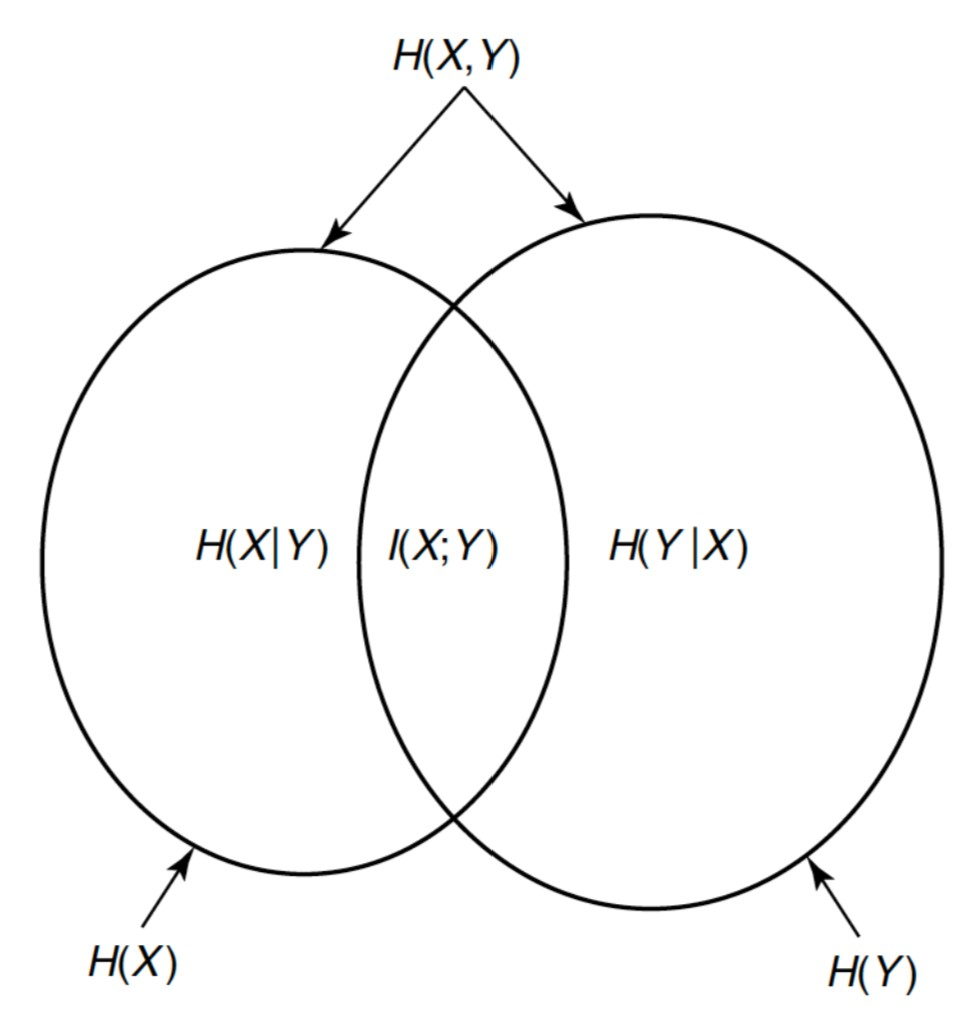
\includegraphics[scale = 0.5]{img/mutual information and entropy.jpg}
		\label{mi}
        \caption{Mutual information and entropy}
\end{figure}

\subsection{Data compression (source coding)}
In this section we introduce the notion of \textbf{source code}.

\image{img/sourceCoding}{Source coding theorem is focused on the first part of the channel.}{0.7}

As we introduced before, because of the presence of noise inside the channel, source and destination also have the task to ensure \textbf{efficiency} and \textbf{reliability} of messages. However, ensuring these two properties introduces another problem: \textbf{redundancy}. In order to achieve efficiency it is necessary to remove redundancy from the messages, using \textbf{compression}; on the other hand, improving reliability requires the receiver to be able to make inferences about the original message, which again can only be achieved through redundancy. As we can see there is an intrinsic \textbf{contrast} between the two requirements, hence it is necessary to find a good \textbf{trade-off}. A possible solution, for instance, is to send more (possibly an odd number of) bits to codify a single symbol (e.g. \verb|"0"| is encoded as \verb|"000"|). In this way the decoder will more easily be able to spot and fix errors in the received message, increasing reliability as well as redundancy.


Let $X$ be random variable with range $\mathcal{X}$:
$$\mathcal{X} = \{x_1, \cdots, x_n\}$$

and probability distribution

$$p(x) = Pr\{X=x\}$$

We define $\mathcal{D}$ as the channel alphabet and we define a code as a function that executes the following transformation:
$$C : \mathcal{X} \rightarrow \mathcal{D}^*$$
, where $\mathcal{D}^*$ represents the set of strings of symbols from the alphabet $\mathcal{D}$. In this sense, a code is a function that maps strings from the source code $\mathcal{X}$ to the channel code $\mathcal{D}$. We denote with $C(x)$ the \textbf{codeword} associated to $x$.

In general, it is clear that not all codes are good ones. However, there are some rules that can help us in order to define a good one:
\begin{itemize}
	\item It must be as \textbf{short} as possible in order to ensure the \textit{efficiency} of transmission.
	\item There must not be presence of codes that are prefixes of other ones: this leads problems with \textit{efficiency} because receiver must wait other bits in order to understand if sender has sent letter $\verb|"b"|$ or $\verb|"d"|$.
\end{itemize}  
It is also possible to have an efficient code that is useless, because receiver can't understand what is transmitted in the channel. An example is the following table in which \textbf{ambiguity} appears.
\begin{table}[H]
	\centering
	\begin{tabular}{| c | c |}
		\hline
		$\mathcal{X}$ & $\mathcal{D}^*$\\\hline
		$\verb|1|$ & $\verb|0|$ \\
		$\verb|2|$ & $\verb|0|$ \\
		$\verb|3|$ & $\verb|0|$ \\
		$\verb|4|$ & $\verb|0|$ \\
		\hline
	\end{tabular}
	\caption{Ambiguous code.}
\end{table}

\subsubsection{Classes of codes}
We can define the following classes of codes:

\begin{enumerate}
    \item \textbf{Non-singular codes}, in which all the codewords are distinct (i.e. the coding function $C$ is injective). Notice that non-singular codes can be not uniquely decodable, as represented below;

    \begin{table}[H]
	\centering
	\begin{tabular}{| c | c |}
		\hline
		$\mathcal{X}$ & $\mathcal{D}^*$\\\hline
		$\verb|1|$ & $\verb|0|$ \\
		$\verb|2|$ & $\verb|010|$ \\
		$\verb|3|$ & $\verb|01|$ \\
		$\verb|4|$ & $\verb|10|$ \\
		\hline
	\end{tabular}
	\caption{Example of non-singular but not uniquely decodable code.}
    \end{table}

    A code like this can generate a message such as $\verb|010|$, in which a decoder can generate more than one decoded message. For instance, it could generate 2, 14 or 31.. As we can see, even if we are in an optimal situation without noise, the receiver can't understand the message it received.

    \item \textbf{Uniquely decodable}, in which any encoded string must have a unique decoding. An example is provided here:

    \begin{table}[H]
	\centering
	\begin{tabular}{| c | c |}
		\hline
		$\mathcal{X}$ & $\mathcal{D}^*$\\\hline
		$\verb|1|$ & $\verb|10|$ \\
		$\verb|2|$ & $\verb|00|$ \\
		$\verb|3|$ & $\verb|11|$ \\
		$\verb|4|$ & $\verb|110|$ \\
		\hline
	\end{tabular}
	\caption{Example of uniquely decodable but not instantaneous code.}
    \end{table}

    \item \textbf{Instantaneous code} or \textbf{Prefix code}, in which no codeword is a prefix of any other. An example is provided here:

    \begin{table}[H]
	\centering
	\begin{tabular}{| c | c |}
		\hline
		$\mathcal{X}$ & $\mathcal{D}^*$\\\hline
		$\verb|1|$ & $\verb|0|$ \\
		$\verb|2|$ & $\verb|10|$ \\
		$\verb|3|$ & $\verb|110|$ \\
		$\verb|4|$ & $\verb|111|$ \\
		\hline
	\end{tabular}
	\caption{Example of instantaneous (or prefix) code.}
    \end{table}
    
\end{enumerate}

Notice that a uniquely decodable code is also non-singular (it is not always true the opposite), and an instantaneous/prefix code is also uniquely decodable: a scheme of the classes of codes is provided here:

\image{img/codesClassification}{Codes classification.}{0.7}

\subsection{Quantifying efficiency}
While we define a code, it is also useful to consider the efficiency given by it. If we consider a code like this:
\begin{table}[H]
	\center
\begin{tabular}{| c | c | c |}
	\hline
	$\mathcal{X}$ & $\mathcal{D}^*_1$ & $\mathcal{D}^*_2$\\\hline
	$\verb|a|$ & $\verb|0|$ & $\verb|0|$ \\
	$\verb|b|$ & $\verb|10|$ & $\verb|10001|$ \\
	$\verb|c|$ & $\verb|110|$ & $\verb|1100110|$ \\
	$\verb|d|$ & $\verb|111|$ & $\verb|1110010|$ \\
	\hline
\end{tabular}
\caption{Non-efficient code.}
\end{table}

, we can see immediately that the codewords use too many bits to codify the original symbol of the source. So we could consider the \textbf{length of codewords} as a \textbf{possible metric} to quantify efficiency of a code, but we will find out in the next example that this metric is not the best one.
\begin{exmp} Consider the following example:
	$$\mathcal{X} = \{a, b, c, d\} \qquad \mathcal{D} = \{0,1\}$$
	with the following probabilities:
	$$p(a) = \frac{1}{2} \qquad p(b) = \frac{1}{4} \qquad p(c) = \frac{1}{8} \qquad p(d) = \frac{1}{8}$$
	We can define two possible codes to convert symbols from $\mathcal{X}$ to $\mathcal{D}$.
	\begin{table}[H]
		\centering
		\begin{tabular}{| c | c | c |}
			\hline
			$\mathcal{X}$ & $\mathcal{D}^*_1$ & $\mathcal{D}^*_2$\\\hline
			$\verb|a|$ & $\verb|0|$ & $\verb|111|$ \\
			$\verb|b|$ & $\verb|10|$ & $\verb|110|$ \\
			$\verb|c|$ & $\verb|110|$ & $\verb|10|$ \\
			$\verb|d|$ & $\verb|111|$ & $\verb|0|$ \\
			\hline
		\end{tabular}
		\caption{Comparing codes.}
	\end{table}
\end{exmp}
The second code is the reversed version of the first one. If we consider only the length of the codewords we can say that in terms of efficiency they are equal, but this is not true. When we talk about efficiency, it is necessary to consider the probability distribution of the symbols. In this example the symbol $\verb|a|$ is very likely to appear, while symbol $\verb|d|$ is very unlikely to be found. In other words, while the second code maps $\verb|a|$ to a long codeword and $\verb|d|$ to a short one, the first code does the opposite, hence proving to be more efficient since it uses, on average, fewer bits.\\
We can thus define the \textbf{length of a code} with the following formula:
		$$ L(C) = \sum_{x \in \mathcal{X}} p(x) l(x) $$
, i.e. it is the average length of the codewords,
where $l(x)$ is the length of the codeword associated to the symbol $x$.

\begin{exmp} Let $X$ be a random variable with following range:
	$$\mathcal{X} = \{1, 2, 3, 4\} \qquad \mathcal{D} = \{0,1\}$$
	and the following probability distribution:
	$$p(X = 1) = \frac{1}{2} \qquad p(X = 2) = \frac{1}{4} \qquad p(X = 3) = \frac{1}{8} \qquad p(X = 4) = \frac{1}{8}$$

Then:

$$
L(C) = \frac{1}{2} \cdot 1 + \frac{1}{4} \cdot 2 + \frac{1}{8} \cdot 3 + \frac{1}{8} \cdot 3 = 1.75
$$

Notice that in this case $H(X) = 1.75 = L(C)$.

\end{exmp}

\begin{exmp} Let $X$ be a random variable with following range:
	$$\mathcal{X} = \{1, 2, 3\} \qquad \mathcal{D} = \{0,1\}$$
	and the following probability distribution:
	$$p(X = 1) = \frac{1}{3} \qquad p(X = 2) = \frac{1}{3} \qquad p(X = 3) = \frac{1}{3}$$

Then:

$$
L(C) = \frac{1}{3} \cdot 1 + \frac{1}{3} \cdot 2 + \frac{1}{3} \cdot 3 = 1.66
$$

However, in this case $H(X) = \log_2 3 = 1.58$ bits.

\end{exmp}

There is a theorem which states that entropy is a lower bound for $L(C)$, considering a \textbf{noise free channel}.

\begin{thm}[Shannon's theorem] 
	Let $X$ be a random variable (source), with range $\mathcal{X}$ and probability distribution $p(x)$. 
	Let $\mathcal{D}$ be the channel's alphabet, $C : \mathcal{X} \rightarrow \mathcal{D}^*$ an instantaneous code for X and $D = |\mathcal{D}|$.\\
	Then, if the channel is noise free: 
	$$ L(C) \geq H_D(X)$$
	where $D$ is the base of the logarithm. 
	
	Moreover:
	$$ L(C) = H_D(x) \iff \forall x \in \mathcal{X}: \quad l(x) = -\log_D p(x) = \log_D \frac{1}{p(x)} $$
\end{thm}

When the probability distribution $p(x)$ has the property:
$$ \log_D \frac{1}{p(x)} \in \mathbb{N}\setminus\{0\}$$
the probability distribution $p(x)$ is called \textbf{D-adic}. Thus, the equality in the theorem is reached if and only if the probability distribution is \textit{D-adic}.

\begin{exmp}
$$\mathcal{X} = \{a, b, c, d\} \qquad \mathcal{D} = \{0,1\}$$
with the following probabilities:
$$p(a) = \frac{1}{2} \qquad p(b) = \frac{1}{4} \qquad p(c) = \frac{1}{8} \qquad p(d) = \frac{1}{8}$$

$$ p(a) = \frac{1}{2} \quad \log_2 2 = 1$$
$$ p(b) = \frac{1}{4} \quad \log_2 4 = 2$$
$$ p(c) = \frac{1}{8} \quad \log_2 8 = 3$$
$$ p(d) = \frac{1}{8} \quad \log_2 8 = 3$$
\end{exmp}

\subsection{Huffman coding}
The \textbf{Huffman coding} is a \textbf{greedy algorithm} used to build/define the \textbf{best code} in a lossless data compression.

The algorithm proceeds as follows:

\begin{enumerate}
    \item Take the two least probable symbols in the alphabet. These two symbols will be given the longest codewords, which will have equal length, and differ only in the last digit;
    \item Combine these two symbols into a single one, and repeat.
\end{enumerate}

\begin{exmp} Huffman coding with $\mathcal{X} = \{x_1, \dots, x_6\}$ and $p(x) = (0.4,0.3,0.1,0.1,0.06,0.04)$.
	
	\begin{table}[H]
		\centering
		\begin{tabular}{| c | c | c | c | c | c | c | c | c | c | c |}
			\hline
			$\mathcal{X}$ & $p(x)$ & $c_5$ & $p(x)^1$ & $c_4$ & $p(x)^2$ & $c_3$ & $p(x)^3$& $c_2$ & $p(x)^4$&$c_1$ \\\hline
			$x_1$ & $0.4$ & $1$ & $0.4$ & $1$ & $0.4$ & $1$ & $0.4$& $1$ & $0.6$& $0$ \\
			$x_2$ & $0.3$ & $0$ & $0.3$ & $00$ & $0.3$ & $00$ & {\color{red}{*$0.3$}}& $00$ & $0.4$& $1$ \\
			$x_3$ & $0.1$ & $011$ & {\color{red}{*$0.1$}} & $011$ & {\color{red}{*$0.2$}} & $010$ & {\color{red}{*$0.3$}}& $01$ & &  \\
			$x_4$ & $0.1$ & $010$ & {\color{red}{*$0.1$}} & $0100$ & {\color{red}{*$0.1$}} & $011$ & & & & \\
			$x_5$ & {\color{red}{*$0.06$}} & $01010$ & $0.1$ & $0101$ & & & & & &\\
			$x_6$ & {\color{red}{*$0.04$}} & $01011$ &  &  &  & & & & & \\
			\hline
		\end{tabular}
		\caption{Comparing codes.}
	\end{table}
\end{exmp}

\begin{thm}[Optimality of Huffman codes]
    Huffman codes are optimal (and instantaneous).
\end{thm}

\begin{thm}
    If $C_{\text{Huffman}}$ is a Huffman $D$-ary code for a random variable $X$, then:

    $$
    H_D(X) \leq L(C_{\text{Huffman}}) < H_D(X) + 1
    $$
\end{thm}

\begin{exmp}
    Let $X$ be a r.v. with range $\mathcal{X} = \{ x_1, x_2 \}$ and $p(x_1) = \frac{2}{3}$ and $p(x_2) = \frac{1}{3}$. Then, the optimal (Huffman) code is :

    $$
    x_1 \xrightarrow{} 0
    $$

    $$
    x_2 \xrightarrow{} 1
    $$

    In this case, the length of the code is 1, and we can't apparently do better than this, but let's consider blocks of two consecutive symbols. Assuming statistical independence, we have $p(x_1, x_1) = \frac{4}{9}$, $p(x_1, x_2) = \frac{2}{9}$, $p(x_2, x_1) = \frac{2}{9}$, $p(x_2, x_2) = \frac{1}{9}$. An optimal (Huffman) code for this new source is :

    $$
    x_1 x_1 \xrightarrow{} 0
    $$

    $$
    x_1 x_2 \xrightarrow{} 10
    $$

    $$
    x_2 x_1 \xrightarrow{} 110
    $$

    $$
    x_2 x_2 \xrightarrow{} 111
    $$

    Now, the expected codeword length per input symbol is 0.944, which is less than before! Clearly, increasing the input size, we obtain better and better codes. Shannon's theorem states that this process will converge towards the entropy of $X$, in this case $H(X) = 0.91830$
    
\end{exmp}

\subsection{Channel}
In the previous sections, we covered the topic of coding. However, two different definitions of codes can be indicated:
\begin{itemize}
	\item \textbf{Lossless codes}, i.e. codes that don't lose any information from the initial source. It is possible to reconstruct completely the original message;
	\item \textbf{Lossy codes}, i.e. codes that lose information. After compression some information is lost (jpg, $\dots$).
\end{itemize}
Two meaningful concepts are \textbf{source coding}, which is related to \textit{efficiency}, and \textbf{channel coding}, that is, instead, related to \textit{reliability}. We will now focus exactly on this last topic. 

\subsubsection{Definition of channel}
A channel can be formally defined as a triplet:
$$\mathcal{C} = (\mathcal{X}, p(y|x), \mathcal{Y})$$
where:
\begin{itemize}
	\item $\mathcal{X}$ is the \textbf{input alphabet}.
	\item $p(y|x)$ is the \textbf{channel's probability distribution}. It represents the probability that symbol $x$ is translated into $y$. It is the most important component of the channel and it is defined as:
	$$p(y|x) = Pr(Y=y | X = x)$$
	\item $\mathcal{Y}$ is the \textbf{output alphabet}.
\end{itemize}
\image{img/channelDef}{Channel definition.}{0.6}

\subsubsection{Capacity of a channel}
Let us consider a channel $\mathcal{C}$, we want to analyze the mutual information $I(X;Y)$. We have defined the mutual information as:
$$I(X;Y) = H(X) - H(X|Y)$$
where:
\begin{itemize}
	\item $H(X)$ is considered as $f(p(x))$ function of the probability distribution of the source.
	\item $H(X|Y) = -\sum_x \sum_y p(x,y) \log{p(x|y)}$, where:
		\begin{itemize}
			\item $p(x,y) = p(x)p(y|x)$ in which $p(x)$ is related to the \textit{source} and $p(y|x)$ is related to the \textit{channel}. Generally, it is possible to say that $p(x,y)$ depends both on the source and on the channel.
			\item From Bayes Theorem we also know that $$p(x|y) = \frac{p(y|x) p(x)}{p(y)}$$ in which again $p(y|x)$ is related to the \textit{channel} and instead $p(x)$ is related to the \textit{source}.
			$$p(y) = \sum_x p(x,y) = \sum_x \underbrace{p(x)}_{source}\underbrace{p(y|x)}_{channel}$$
		\end{itemize} 
\end{itemize}
The mutual information that travels on the channel depends both on the source and on the channel.
$$I(X;Y) = f(p(x), p(y|x)) = f(source, channel)$$
where:
\begin{itemize}
	\item $p(x)$ is the ``a priori''  probability.
	\item $p(y|x)$ is the ``a posteriori'' probability.
\end{itemize}
This means that we can't use mutual information to give capacity information of the channel since $I(x,y)$ is not only dependent on the channel itself, but also on the source.	
After all these premises, we are able to define the \textbf{capacity of channel} as:
$$C = \max_{p(x)} I(X;Y)$$

The \textbf{capacity} represents the maximum value of mutual information given by all the possible probability distributions of the source. 
\begin{exmp}
	We compute the capacity of the following Binary Symmetric Channel:\\
	\image{img/exampleCapacity}{Binary symmetric channel.}{0.6}
	We know that $P\{X=0\} = \pi$ and $P\{X=1\} = 1-\pi$ (with $\pi \in [0,1]$).

What could happen in the different extreme cases is explained in the following lines:
\begin{itemize}
	\item $p = 0$, we have that the channel is \textbf{perfect} and its capacity is 1. This represent the ideal case in which the channel is not affected by noise and receiver knows that the messages are correct. No loosing of information.
	\image{img/p0}{Channel representation when $p=0$.}{0.3}
	
	\item $p = 1$, we have that the channel is again \textbf{perfect}. Receiver always knows how to reconstruct the right message. The message is always modified during the transmission on the channel. The channel's capacity is again 1.
	\image{img/p1}{Channel representation when $p=1$.}{0.3}
	
	\item $p=0.5$ is the worst scenario for the receiver. We can consider the starting message $X$ and the final message $Y$ as independent messages.
	\image{img/p05}{Channel representation when $p=0.5$.}{0.3}
\end{itemize}
\end{exmp}
Here there is a strong assumption: the \textbf{receiver knows the probability distribution of the channel.}
The best case for the receiver is to know both the channel distribution and the sender distribution, but this is not always feasible.
Probabilities of the channel, in fact, can be specified only after several trials and they are not fixed, as they could change during the time.

\subsection{Reliability}
When we have a noisy channel, the simplest way to improve reliability is exploit the \textbf{repetition of the code}, i.e. add redundancy to the code, in order to reduce the probability of errors during the communication.

\begin{figure}[h!]
		\centering
        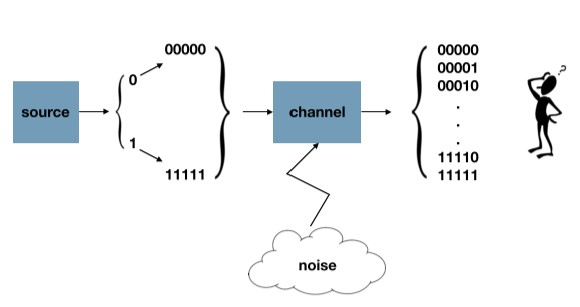
\includegraphics[scale = 1.5]{img/redundancy.jpg}
		\label{mi}
        \caption{Adding redundancy in a noisy channel}
\end{figure}

Notice that in this case the receiver decides how to decode the redundant message by taking, for example, a majority vote. Assume that a channel is BSC with error probability $p = 10^{-2}$. Then, using a repetition code of length 3, we reduce this error probability to $3 \cdot 10^{-4}$, but at the same time we reduced the transmission rate to $\frac{1}{3}$.

If we use a repetition code of length 5, we reduce the probability of error to approximately $10^{-5}$, reducing the transmission rate to $\frac{1}{5}$.

What if we now consider $n \rightarrow \infty$? Let's define $P_e$ as the error probability. When $n \rightarrow \infty$ we have that $P_e \rightarrow 0$ but $R \rightarrow 0$, meaning that a more reliable code produces a slower communication system.
It is necessary to find a right trade-off to maintain a good level of reliability and speed.

\subsection{Channel coding theorem - Shannon's 2nd theorem}
\begin{thm}[Channel coding theorem]
	Let $\mathcal{C}$ be a channel with capacity $C$.
	\begin{itemize}
		\item If $R < C$, there exists a sequence of codes with transmission rate $R$ such that:
		$$P_e  \underset{n \rightarrow \infty}{\rightarrow} 0$$

        \item Conversely, if a sequence of codes transmitting at rate $R$ has a probability error approaching to zero (i.e. $P_{e} \rightarrow 0$), then $R \leq C$. 
        \end{itemize}
\end{thm}

In this sense, this theorem states that we can send a message \textbf{at a finite rate} through a noisy channel with error probability \textbf{as small as we want}, provided that we transmit at a rate smaller than the capacity. Thus, the \textbf{capacity} of the channel is an \textbf{upper bound} for $R$ if we want to define a reliable code.

\section{Neural Networks}

A Neural Network is an information processing paradigm that is inspired by the way biological nervous systems, such as the brain, process information. The key element of this paradigm is the new structure of the information processing system. It is composed of a large number of highly interconnected processing elements (\textbf{neurons}) working in unison to solve specific problems. A NN is configured for a specific application, such as pattern recognition or data classification, through a learning process.\\
Two key \textbf{features} distinguish neural networks from any other sort of computing developed:

\begin{itemize}
	\item \textbf{Neural networks are adaptive or trainable}. Neural networks are not so much programmed as they are trained with data. The more data they are fed, the more accurate or complete is their response;
	\item \textbf{Neural network are naturally massively parallel}. This suggests they should be able to make decisions at high-speed and be fault tolerant (information is stored in a distributed fashion). 
\end{itemize}

\subsection{Biological digression}
As we introduced before, the functioning of a Neural Network is highly inspired by the way in which the neural system and the brain process the information. The biological neural network is composed by the following elements:

\image{img/neural_dynamics}{Neural dynamics.}{0.6}


\begin{itemize}
	\item \textbf{Cell body (Soma)}: 5-10 microns in diameter, it represents the \textit{computational unit};
	\item \textbf{Axon}: it represents the output mechanism for a neuron. A single axon may be connected to thousands of branches and cells;
	\item \textbf{Dendrites}: they receive incoming signals from other nerve axons via synapse;
	\item \textbf{Synapses}: they represents the junctions (``connecting points'') between neurons, i.e. the point in which a neuron's axon passes the information to the "next" neuron's dendrite.
\end{itemize}

The \textbf{transmission of signal} in the cerebral cortex is a complex process:
$$\text{Electrical} \rightarrow \text{Chemical} \rightarrow \text{Electrical}$$
Simplifying:
\begin{enumerate}
	\item The cellular body performs a "\textit{weighted sum}" of the incoming signals.
	\item If the result exceeds a certain threshold value, then it produces an "action potential" which is sent down the axon (cell has "fired"), otherwise it remains in a rest state.
	\item When the electrical signal reaches the synapse, it allows the ``neuro-transmitter'' (chemical) to be released. This combines with the ``receptors'' in the post-synaptic membrane.
	\item The post-synaptic receptors provoke the diffusion of an electrical signal in the post-synaptic neuron. 
\end{enumerate}
In summary, computations by neuron are performed thanks to a combination of electrical and chemical processes. 

A very important concept of the neural system is the so-called \textbf{synaptic efficacy}, which can be defined as the amount of electricity that enters into the post-synaptic neuron, compared to the action potential of the pre-synaptic neuron. The \textbf{learning step} takes place by modifying the synaptic efficacy. In general, two different types of synapses are present:
\begin{itemize}
	\item \textbf{Excitatory}, which favor the generation of action potential in the post-synaptic neuron, i.e. they tend to increase the energy;
	\item \textbf{Inhibitory}, which hinder the generation of action potential, so they de-amplify the signal.
\end{itemize}

\subsection{The McCulloch and Pitts Model (1943)}

Neural network simulations appear to be a recent development; however, this field was established before the advent of computers and the first model, which was created in 1943, is the \textbf{McCulloch and Pitts Model}.\\
The McCulloch-Pitts (MP) neuron is a simple process unit modeled as a binary threshold unit.

\image{img/MP_neuron}{McCulloch and Pitts neuron representation.}{0.55}


\textbf{Input} = $x$ = $\sum_j w_jI_j$. \\
\textbf{Output} = $g(x) = \begin{cases}
0 \quad \text{if }x<T\\
1 \quad \text{if }x \geq T
\end{cases}$

In this sense, we can rewrite the output as:

$$
y = g\left(\sum_j w_jI_j - T\right) 
$$

\textbf{NOTE}:

\begin{itemize}
    \item the MP neuron fires if the input $x$ = $\sum_j w_jI_j$ exceeds a certain threshold $T$, called \textbf{claiming parameter};

    \item the function $g(.)$ is also called \textbf{activation function} or \textbf{unit step function}, and it is a non linear function;

    \item the weight $w_{ij}$ represents the strength of the synapse between neuron $i$ and neuron $j$. 
\end{itemize}

\subsubsection{Properties}

By properly combining MP neurons, it is possible to simulate the behavior of any boolean circuit:

\image{img/MP_properties}{Three elementary logical operations (\textit{a}) \textbf{negation}, (\textit{b}) \textbf{and}, (\textit{c}) \textbf{or}. In each diagram the states of the neurons on the left are at time $t$ and those on the right at time $t+1$.}{0.65}

Notice that it is not possible to build a NN for the \textit{XOR} operator using a single neuron.

\subsection{Network topologies and Architectures} There are different network topologies and the main differences are highlighted below.

\begin{table}[H]
	\centering
	\begin{tabular}{| p{7.5cm} | p{7.5cm} |}
		\hline
		\textbf{Feed-forward only}: allow signals to travel one way only: from input to output, so it has connections only in one direction. This topology forms a direct acyclic graph, and its outputs are deterministic functions of the input & \textbf{Recurrent networks}: can have signals traveling in both directions by introducing loops in the network. Feedback networks are powerful and can get extremely complicated, since their output depends on the initial state, which in turn depends on previous outputs.\\
		\hline
		\textbf{Fully connected}: each neuron of a layer is connected to every neuron in the previous layer, and each connection has it's own weight. & \textbf{Sparsely connected}: has fewer links than the possible maximum number of links within that network.  \\
		\hline
		\textbf{Single layer}: every neuron connects directly from the network's input to its output & \textbf{Multi-layer}: it has one or more layer of hidden neurons that are not connected to the output.\\
		\hline
	\end{tabular}
\end{table} 
\image{img/feedforward}{\textit{(a)} feedforward network - \textit{(b)} feedback network}{0.65}

In general, there are problems which are more suited to be solved with a \textit{feedforward NN} than a \textit{recurrent NN} or vice-versa, for example a task of image classification, i.e. assigning a label to an input image, can be easily solved with a \textit{feedforward NN}, whereas a task of image captioning, i.e. provide a verbal description of the input image, is more suitable to be solved with a \textit{recurrent NN}, since the length of the output is not known in advance. 


\subsection{Classification problems}
Given:

\begin{enumerate}

	\item a set of \textbf{features} $\{f_1,f_2,\dots,f_n\}$ , which represents the attributes that describe our objects;
	\item a set of \textbf{classes} $\{c_1,\dots,c_m\}$, which represents the categories in which the objects are divided
 
\end{enumerate}

, the \textbf{goal} of the \textbf{classification} problem is to classify the \textbf{objects} according to their \textbf{features}. The geometric interpretation of this task is to represent the features in the space and try to separate the classes by finding the closest objects.

\image{img/nn1.jpg}{Classification problem}{0.7}

\subsubsection{Neural networks for classification}

A neural networks can be used as a classification device and it can be configured as follow:

\begin{itemize}

	\item the \textit{input} of the network are the object's \textbf{features} to classify.
 
	\item the \textit{output}, returned by the network, is the \textbf{class} predicted for the input object.
 
\end{itemize}

Before going on we assume that features are numbers, and remember that we cannot map categorical features into numbers, since we would introduce an order, which would lead to mistakes. For instance: red = 0, blue = 1, green = 2 would not be a correct coding since we would be imposing a non-existent order between colors. We propose a simple model of neural network:

\image{img/NN_1}{Example of NN with 3 features input and 2 class labels as output.}{0.4}

The application of a learning algorithm of a network configuration consists in finding the best configuration of weights of the incoming connection and the threshold. In these classification problems we can get rid of the \textbf{thresholds} (also called biases) associated to neurons by adding an extra input \textbf{permanently clamped at -1}. By doing so,\textbf{ thresholds become weights} and can be adaptively adjusted during learning phase, otherwise we would have to manually tune the right threshold. In this way, the output $y$ of the network becomes:

$$
y = g\left(\sum\limits_{i = 1}^{n+1} w_ix_i\right)
$$
, where $x_{n+1} = -1$.

\begin{figure}[h!]
		\centering
        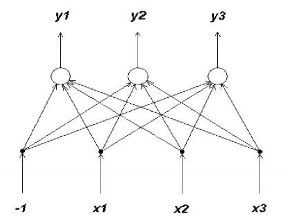
\includegraphics[scale = 1.5]{img/thresholds.jpg}
		\label{mi}
        \caption{We can remove thresholds by adding an input neuron clamped at -1}
\end{figure}

\subsubsection{The Perceptron}
The perceptron is a \textbf{linear classifier} consisting of a \textbf{single layer of MP neurons} connected in a \textbf{feedforward} way, i.e. it is a \textbf{single-layer feedforward NN}. A simple perceptron can only solve linearly separable problems, and this makes the model very limited in terms of computational power. 

\image{img/percep1.jpg}{Representation of a perceptron}{0.5}

The perceptron is characterized by the following properties:

\begin{itemize}
    \item The output is $-1/+1$, while using the MP neurons we had $0/1$;
    
    \item It is capable of learning from examples;
    
    \item From a geometrical point of view, the perceptron identifies a linear boundary between two classes:

    \image{img/percep2.jpg}{Geometry interpretation of the perceptron}{0.5}

    In this case, the hyperplane (line) $w_1x_1 + w_2x_2 - b$ represents a linear decision boundary for a two-dimensional, two-classes classification problem. If $w_1x_1 + w_2x_2 - b > 0$ then the predicted class is 1, otherwise is 0. Obviously, if we change the parameters $w_1$, $w_2$ and $b$, we get a different boundary.
    
\end{itemize}

\paragraph*{The Perceptron Learning Algorithm.} The goal of this algorithm is to find the best weights and parameters in order to separate the objects of the classes. It is an iterative algorithm characterized by the following variables and parameters:
\begin{itemize}

	\item $x(n) \in \mathbb{R}^{m+1}$, the \textbf{input vectors}. They are $(m+1)\text{-by-1 vectors} = [-1, x_1(n), x_2(n), \dots, x_m(n)]^T$\\
	Objects are described with $m$ features and -1 as the threshold, which is the reason why the input vectors have size $m+1$;
 
	\item $w(n) \in \mathbb{R}^{m+1}$, the \textbf{weights vectors}. They are $(m+1)\text{-by-1 vectors} = [b, w_1(n), w_2(n), \dots, w_m(n)]^T$;
 
	\item $b$, the \textbf{bias};
 
	\item $y(n)$, the \textbf{actual response} of the NN (quantized). $y(n) \in \{ +1, -1 \}$;
 
	\item $d(n)$, the \textbf{desired response} from the dataset. $d(n) \in \{ +1, -1 \}$;
 
	\item $\eta$, the \textbf{learning-rate parameter}, a positive constant strictly smaller than $1$. It affects the convergence of the learning algorithm. 
\end{itemize}

The algorithm works as follows:

\begin{enumerate}

	\item \textbf{Initialization.} Set $w(0) = 0$ and then perform the following computations for time-step $n=1,2,\dots$.
 
	\item \textbf{Activation.} At time-step $n$, activate the perceptron by applying continuous-valued input vector $x(n)$ and desired response $d(n)$ (both picked from the training set).
 
	\item \textbf{Computation of the actual response.} Compute the actual response of the perceptron as:
	$$y(n) = sgn[w^T(n)x(n)] \qquad w^Tx = \sum_iw_ix_i$$
	where $sgn(\cdot)$ is the signum function ($+1$ if the argument is greater or equal to $0$, $0$ otherwise). Notice that, so far, no learning phase has taken place.
 
	\item \textbf{Update of the weight vector.} Update the weight vector of the perceptron to obtain:
	$$w(n+1) = w(n) + \eta[d(n) - y(n)]x(n)$$
	where
	$$d(n) = 
	\begin{cases}
	+1 \qquad \text{if } x(n) \text{ belongs to class } \varphi_1\\
	-1 \qquad \text{if } x(n) \text{ belongs to class } \varphi_2 
	\end{cases}$$
	This is where the learning phase takes place: in case of wrong classification, the current configuration will change modifying $d(n) - y(n)$, if the network classifies $x(n)$ correctly, then there is no learning as $d(n)-y(n) = 0$. The convergence of the algorithm is ensured by $x(n)$. Note that $x(n)$ is included to be sure that the new prediction is correct, but the updated weights could fail to classify another input vector (even an already seen one).
 
	\item \textbf{Continuation.} Increment time step $n$ by one and go back to step 2.
 
\end{enumerate}

In practice, this algorithm is trying to find the best possible straight line (or hyperplane) which separates the ``good'' examples from the ``bad'' ones. The decision boundary is described such that $w_1x_1 + w_2x_2 = 0$ and, in general, each point is classified according to the following conditions:  $w_1x_1 + w_2x_2 \geq 0$ and $w_1x_1 + w_2x_2 < 0$

\image{img/perceptron_algorithm}{Perceptron learning algorithm procedure.}{0.50}

From a geometrical point of view, finding $w$ means finding the line (or hyperplane) which separates the two regions.
As we can see from the previous image, some examples can be misclassified. For each weights update, a specific error is corrected but other mistakes in classification may arise because of the changes in the weights. By iteratively adjusting the weights, a final and ``stable'' solution can be reached.\\
It is possible to define a \textbf{decision region} as an area in which all the samples of one class fall. A classification problem is said to be \textbf{linearly separable} if the decision regions can be separated by an hyperplane. These concepts allow us to introduce one important \textbf{limitation of perceptrons}: they can only solve linearly separable problems.

\paragraph*{The Perceptron Convergence Theorem.} This theorem was formulated by Rosenblatt in 1960. It states the following: if the training set is \textbf{linearly separable}, the perceptron learning algorithm \textbf{always converges} to a consistent hypothesis after a \textbf{finite} number of epochs, i.e. an entire presentation of the dataset, for any $\eta > 0$ (Note: nothing is said with respect to the number of steps).\\
If the training set is \textbf{not linearly separable}, after a certain number of epochs the weights will start oscillating. In this situation some points will surely be misclassified. The learning algorithm will never converge to a stable configuration, due to the fact that the perceptron can't solve non-linear classification problems.

\par \bigskip \noindent
\subsection{Multi-Layer Feed-forward Neural Networks}
In the following image it is possible to find some properties of the different structures that can create a neural network.

\image{img/role_units}{A view of the Role of Units}{0.86}

As we said before, the limit of the perceptron algorithm is that it can only deal with linearly separable problems. In order to overcome these limitations, the introduction of \textbf{multi-layer feed-forward networks} allows us to improve our networks through the addition of \textbf{hidden layers} between the input and the output layer. This allows us to reach a good approximation on our classification problem: it is possible to notice that a network with just one hidden layer can represent any Boolean function, including XOR. One property of such networks is the \textbf{universal approximation power}, which states that a 2-layers network (one input layer, one hidden layer) can approximate any smooth function (valid for regression problems), provided that the hidden layer is large enough.

\image{img/fNN.png}{Neural Network function model.}{0.65}		


\paragraph*{Continuous-valued units.} The usage of continuous-valued units allows us to introduce calculus and derivative procedures that will give us several advantages.\\ 
The \textbf{activation function} of continuous-valued units is \textbf{sigmoid} (or logistic), which means that neurons can now fire with different intensities, not only 0/1. In this sense, their output is not boolean, but it belongs to the continuous range between $0$ and $1$. These values are often interpreted as probabilities.
$$g \rightarrow \sigma(x) = \frac{1}{1+e^{-f(x)}} \in (0,1)$$
\image{img/sigmoid}{Sigmoid function.}{0.51}
Thus, continuous-valued discriminant functions allow us to have some measure of \textbf{confidence} about the \textbf{prediction}. We will see later on that they are used for \textbf{finding optimal solutions through the gradient descent technique}. In particular, when the $g(z)$ is close to zero (less confidence about the prediction) the gradient will be greater then the situation in which $|g(x)| >> 0$ (more confidence, weights could remain stable).

Another possible activation function is the \textbf{hyperbolic tangent} ($tanh$), which is a rescaling of the logistic sigmoid such that its output range is from -1 and 1. 
$$g \rightarrow \sigma(x) = \frac{e^{f(x)} - e^{-f(x)}}{e^{f(x)} + e^ {-f(x)}} \in (-1, 1)$$
\image{img/hyperbolic}{Hyperbolic tangent function.}{0.45}


\subsection{Back-propagation learning algorithm}
In this section we introduce the \textbf{backpropagation}, an algorithm for learning the weights in a feed-forward multilayers neural network. 

Let $\mathcal{L} = \{(x_1, y_1), \dots, (x_n,y_n) \}$ be a \textbf{training set}, where $X = \{ x_1, x_2, .., x_n \}$ represents the network \textbf{input} vector and $Y = \{ y_1, y_2, .., y_n \}$ represents the \textbf{desired} network \textbf{output} vector. The algorithm is based on \textbf{gradient descent} method, and it can be seen as a greedy algorithm with infinite possible solutions, in which at each step the best solution is chosen. The algorithm is guaranteed to converge only to a local maximum and during the execution we move along the gradient through a predetermined step-size. This property is given by the fact that this algorithm is just an approximation based on a greedy solution.

\image{img/backpropagation}{Back-propagation schema. $W^l_{ij}$ represents the weight on connection between the $i^{th}$ unit in layer $(l-1)$ to $j^{th}$ unit in layer $l$.}{0.70}

\paragraph*{Supervised learning.} Supervised learning algorithms require the presence of \textbf{previous knowledge} that makes it possible to provide the \textbf{right answers} to the input ``questions''. Technically this means that we need a \textbf{training set} of the form:

$$
\mathcal{L} =\left\{\left(x^1, y^1 \right), \dots , \left(x^N, y ^N \right) \right\}
$$

where:

$$x^\mu (\mu=1,\dots, N) \text{ is the network \textbf{input} vector}$$
$$y^\mu (\mu=1,\dots, N) \text{ is the \textbf{desired} network \textbf{output} vector}$$

The learning (or \textbf{training}) phase consists in determining a configuration of \textbf{weights} such that the \textbf{network output} should be \textbf{as close as possible} to the \textbf{desired output} as many times as possible, for all the examples in the training set. Normally, this amounts to minimizing an \textbf{error function} such as the \textbf{MSE} (Mean Squared Error) function:
$$E(w) = \frac{1}{2} \sum_{\mu} \sum_{k} \left(y_k^\mu - O_k^\mu(w)\right)^2$$
where $O_k^\mu(w)$ is the \textbf{output} provided by the \textbf{output unit $k$} when the network is given example $\mu$ as \textbf{input}. In other words, $O_k^\mu(w)$ represents the prediction of the $k^{th}$ unit when the input is $\mu$. 

The loss function computes the difference between the network output and the expected output and of course, our aim is to \textbf{minimize the loss function} (i.e. solve $min_w E(w)$), which means \textbf{finding the set of weights that minimizes the function}: if the network is performing well, then $E(w$ is close to zero.

In order to minimize the error function $E$, we can use the classic \textbf{gradient descent} algorithm. The gradient gives information about the \textbf{best path to follow} in order to \textbf{maximize/minimize our objective function}. Without any kind of direction information it would be extremely complex to find the solution since we would have to search along an infinite number of directions in a continuous domain. Gradient descent is a very well-known \textbf{greedy algorithm}. It is not guaranteed to find a globally optimal solution, but it works well in finding \textbf{local optima}. 

More specifically, the gradient descent updates the a point by moving along the the direction given by the gradient by a finite step. In the case of the back-propagation algorithm, we have that:
$$w_{ji}^{\text{NEW}} \leftarrow w_{ji}^{\text{OLD}} - \eta \frac{\partial E}{\partial w_{ji}}$$

or

$$\Delta w_{ji} \leftarrow  - \eta \frac{\partial E}{\partial w_{ji}^{\text{OLD}}}$$

, where :

\begin{itemize}
    \item $\Delta w_{ji} = w_{ij}^{\text{NEW}} - w_{ji}^{\text{OLD}}$
    \item $w_{ji}^{\text{NEW}}$ represent the weights between unit $i$ and unit $j$, and they are updated using the gradient of the loss function $E$ computed w.r.t. $w_{ji}^{\text{OLD}}$;
    \item $\eta$ represents the \textbf{learning rate}, i.e. how much the weights are updated at each iteration of the gradient descent method. We will discuss about the possible values of this parameter later in the section;
\end{itemize}

Now we need to define a method for computing the partial derivatives of the loss function efficiently.

To compute the partial derivatives we use the \textbf{error back propagation} algorithm, which consists of two stages:

\begin{itemize}
	\item \textbf{Forward pass}: the \textbf{input} of the network is \textbf{propagated} layer after layer in \textbf{forward} direction.
	\item \textbf{Backward pass}: the \textbf{error} (e.g. MSE) made by the network is \textbf{propagated} \textbf{backward} and \textbf{weights} are \textbf{updated} properly. Thus, the partial derivatives of the errors are computed, and the weights are updated following the gradient descent strategy we defined above. An important thing to underline is that in order to update each weight, we only need a \textbf{local information}, not a global information of all the network.
\end{itemize}


Intuitively, we could say that we determine the gradient direction and then we move in the opposite direction since we want to minimize the error.

\paragraph*{Notation.} Before understanding how the weights are updated, it is important to introduce some notation that will be used later:

\begin{itemize}
    \item $x_k$ represents an input neuron of the network;
    \item $w_{jk}$ represents a weight between the input $x_k$ and the neuron $V_j$ in the middle layer;
    \item $V_j$ represents a neuron in the hidden layer;
    \item $W_{ij}$ represents a weight between a neuron in the hidden layer $V_j$ and the output neuron $O_i$;
    \item $O_i$ represents a output neuron.
\end{itemize}

\imageb{img/notations}{0.5}

Given a pattern $\mu$, an hidden unit $j$ receives a net input
$$h _ { j } ^ { \mu } = \sum _ { k } w _ { j k } x _ { k } ^ { \mu }$$
and produces as output:
$$V _ { j } ^ { \mu } = g \left( h _ { j } ^ { \mu } \right) = g \left( \sum _ { k } w _ { j k } x _ { k } ^ { \mu } \right)$$
The output of a neuron in the output layer is defined as:
$$O _ {i} ^ {\mu} = g(\sum _ k W_{ik} \cdot V _ {k} ^ {\mu})$$


\paragraph*{Updating hidden-to-output weights.} The \textbf{updating rules} of the back-propagation algorithm are nothing but a \textbf{long series of chain rules}. For this reason, the objective function is not linear, hence the output is highly non linear. Indeed, the output is a chain of products of non-linear functions.\\
\begin{equation} \notag
\begin{split}
\Delta W_{ij} &= -\eta \frac{\partial E}{\partial W_{ij}} \quad \text{Replace the error function with its actual expression}\\
&= -\eta \frac{\partial}{\partial W_{ij}} \left[\frac{1}{2} \sum_{\mu} \sum_k (y_k^\mu - O_k^\mu)^2\right] \quad \text{First application of the chain rule}\\
&= \eta \sum _{\mu} \sum_{k} \left(y_{k}^{\mu} - O_{k}^{\mu} \right) \frac{\partial O_{k}^{\mu}} {\partial W_{ij}} \quad \text{The sum over } k \text{ disappears because the partial derivative is}\\
& \hspace*{13.5em} \text{different from 0 only when }k=i \\
&= \eta \sum_{\mu} \left(y_{i}^{\mu} - O_{i}^{\mu} \right) \frac{\partial O_{i}^{\mu}} {\partial W_{ij}} \qquad \text{Again we apply the chain rule. Partial derivative can be}\\
& \hspace*{12.6em} \text{written as } W_{ij} \rightarrow h_i^\mu \rightarrow g'(h_i^\mu)\\
&= \eta \sum _ { \mu } \left( y _ { i } ^ { \mu } - O _ { i } ^ { \mu } \right) g ^ { \prime } \left( h _ { i } ^ { \mu } \right) V _ { j } ^ { \mu } \qquad \text{That is } \frac{\partial h_i^\mu}{\partial W_{ij}} = \frac{\partial}{\partial W_{ij}}\left(\sum_l W_{il} V_l \right) = V_j \frac{\partial W_{ij}}{\partial W_{ij}} = V_j\\
&= \eta \sum _ { \mu } \delta _ { i } ^ { \mu } V _ { j } ^ { \mu } \qquad \qquad where: \quad \delta _ { i } ^ { \mu } = \left( y _ { i } ^ { \mu } - O _ { i } ^ { \mu } \right) g ^ { \prime } \left( h _ { i } ^ { \mu } \right)
\end{split}	
\end{equation}
In $\eta \sum_{\mu} \delta_{i}^{\mu} V_{j}^{\mu}$, component $\delta_{i}^{\mu}$ represents the error made by the $i$-th neuron, whilst $V_{j}^{\mu}$ is the output of the neuron.  

\paragraph*{Updating input-to-hidden weights.}
\begin{equation} \notag
\begin{split}
\Delta w _ { j k } &= - \eta \frac { \partial E } { \partial w _ { j k } } \\
&= \eta \sum _ { \mu } \sum _ { i } \left( y _ { i } ^ { \mu } - O _ { i } ^ { \mu } \right) \frac { \partial O _ { i } ^ { \mu } } { \partial w _ { j k } } \qquad \text{Chain rule}\\
&= \eta \sum _ { \mu } \sum _ { i } \left( y _ { i } ^ { \mu } - O _ { i } ^ { \mu } \right) g ^ { \prime } \left( h _ { i } ^ { \mu } \right) \frac { \partial h _ { i } ^ { \mu } } { \partial w _ { j k } } \qquad \text{Chain rule}
\end{split}
\end{equation}
We have that the partial derivative is:
\begin{equation} \notag
\begin{split}
\frac { \partial h _ { i } ^ { \mu } } { \partial w _ { j k } } &= \sum _ { l } w_{ i l } \frac { \partial V _ { l } ^ { \mu } } { \partial w_{ j k } }\\
&= w_ { i j } \frac { \partial  V_ { j } ^ { \mu } } { \partial  w _ { j k } }\\
&= w_{ i j } \frac { \partial g \left( h _ { j } ^ { \mu } \right) } { \partial w _ { j k } }\\
&= w_{ i j } g ^ { \prime } \left( h _ { j } ^ { \mu } \right) \frac { \partial h _ { j } ^ { \mu } } { \partial w _ { j k } }\\
&= w_{ i j } g ^ { \prime } \left( h _ { j } ^ { \mu } \right) \frac { \partial } { \partial w _ { j k } } \sum _ { m } w _ { j m } x _ { m } ^ { \mu }\\
&=  w_{ i j } g ^ { \prime } \left( h _ { j } ^ { \mu } \right) x _ { k } ^ { \mu }
\end{split}
\end{equation}
Hence coming back to the original equation we have that:
\begin{equation}
\begin{split}
\Delta w _ { j k } &= \eta \sum _ { \mu , i } \left( y _ { i } ^ { \mu } - O _ { i } ^ { \mu } \right) g ^ { \prime } \left( h _ { i } ^ { \mu } \right) w_ { i j } ~g ^ { \prime } \left( h _ { j } ^ { \mu } \right) x _ { k } ^ { \mu }\\
&= \eta \sum _ { \mu , i } \delta _ { i } ^ { \mu } w_ { i j } g ^ { \prime } \left( h _ { j } ^ { \mu } \right) x _ { k } ^ { \mu }\\
&= \eta \sum _ { \mu } \hat { \delta } _ { j } ^ { \mu } x _ { k } ^ { \mu } \qquad \qquad where: \quad \hat { \delta } _ { j } ^ { \mu } = g ^ { \prime } \left( h _ { j } ^ { \mu } \right) \sum _ { i } \delta _ { i } ^ { \mu } w_ { i j }
\end{split}
\end{equation}
$\sum_{i} \delta_{i}^{\mu} W_{ij}$ is the average error performed by the output layer and $i$ is the reference to the $i$-th neuron.\\
In the following image it is possible to understand the error back-propagation. The black lines correspond to the forwarded signals, while the red lines indicate the error that is back-propagated.
\image{img/error_backpropagation}{Error Back-propagation representation.}{0.6}

\paragraph*{Locality of back-propagation.} Another important aspect is the \textbf{locality} of the back-propagation algorithm.

\image{img/locality_backpropagation}{Locality of back-propagation}{0.2}

There exist two different ways of implementing a back-propagation algorithm: off-line and on-line. In the \textbf{off-line} way we compute the gradient exactly, so in order to update a single weight in the network, we need to present all the examples of the training set. This procedure is not generally used because it is computationally expensive.

$$
\Delta \omega_{pq} = \eta \sum_{\mu} \delta_{p}^{\mu} V_{q}^{\mu} \qquad \qquad \text{off-line}
$$
$$
\delta_{p}^{\mu} = \text{Error} \quad V_{q}^{\mu} = \text{Output of neurons}
$$

In the \textbf{on-line} way some noise is introduced, in the sense that the weights are updated at any presentation of an example of the training set.

$$
\Delta \omega_{pq} = \eta\delta_ {p}^{\mu} V_{q}^{\mu} \qquad \qquad \text{on-line}
$$

A possible compromise between the two techniques is called \textbf{stochastic gradient descent}, in which the first technique is used with a randomly selected subset of the training set: in this sense, the gradient changes according to the random choice of the subset. This solution represents a very good method, since on the one hand modern datasets are huge, so updating the weights after the presentation of all the training examples is very expensive, and on the other the randomness through which the subset is selected may help in finding a global maximum/minimum.

\paragraph*{The Back-Propagation algorithm.} In this implementation we will consider the \textbf{on-line} approach. Suppose we have a network with $M$ layers, and let

\begin{itemize}
    \item $V_i^m$ be the output of the $i$-th unit of layer $m$;
    \item $w_{ij}^m$ be the weight on the connection between $j$-th neuron of layer $m-1$ and $i$-th neuron in layer $m$. 
\end{itemize}
  
The general structure of the algorithm is the following:

\begin{enumerate}
	\item Initialize the weight to (small) random values. The choice of small values is made to avoid the derivative of the logistic function being all zeros;
	\item Choose a pattern $\bar{x}^\mu$ and apply it to the input layer $(m=0)$, i.e.:
	$$V _ { k } ^ { 0 } = x _ { k } ^ { \mu } \qquad \forall k$$
	\item Propagate the signal forward (\textbf{Forward pass}):
	$$V _ {i} ^ { m } = g \left( h _ { i } ^ { m } \right) = g \left( \sum _ { j } w _ { i j } V _ { j } ^ { m - 1 } \right)$$
	\item Compute the $\delta$'s for the output layer (\textbf{Backward pass}):
	$$\delta _ { i } ^ { m } = g ^ { \prime } \left( h _ { i } ^ { m } \right) \left( y _ { i } ^ { m } - V _ { i } ^ { m } \right)$$
	\item Compute the $\delta$'s for all preceding layers (for each neuron):
	$$\delta _ { i } ^ { m - 1 } = g ^ { \prime } \left( h _ { i } ^ { m - 1 } \right) \sum _ { j } w _ { j i } ^ { m } \delta _ { j } ^ { m }$$
	\item Update connection weights according to the error, with learning rate $\eta$:
	$$w _ { i j } ^ { N E W } = w _ { i j } ^ { O L D } + \Delta w _ { i j } \qquad \text { where } \quad \Delta w _ { i j } = \eta \delta _ { i } ^ { m } V _ { j } ^ { m - 1 }$$
	\item Go back to step 2 until convergence, i.e. until $\Delta w _ { i j } = 0$. In real implementation we claim $||\Delta w _ { i j }||^2 < \epsilon$, or to stop after a finite number of epochs.
\end{enumerate}

One of the most challenging problems is the choice of the \textbf{learning rate} $\eta$. When $\eta$ is \textbf{small} the algorithm will converge but in a very \textbf{slow} way; on the other hand, when it is too \textbf{big}, there will be an \textbf{oscillating problem} that won't bring the algorithm to the convergence. \\
In the following image we can see the difference in convergence between the same algorithm run with different values of $\eta$. From left to right, they are $0.02, 0.0476, 0.049, 0.0505$.
\image{img/learning_rate}{The Role of the Learning Rate. The minimum is at the $+$ and the ellipse shows a constant error contour.}{0.9}
We can observe that the first case is too slow in reaching the minimum, while in the second and in the third case the oscillation becomes smaller and smaller. Finally, in the last case, the algorithm won't converge, as the oscillation becomes larger and larger.\\

One possible remedy to this problem is in introducing the \textbf{momentum term}, a simple \textbf{heuristic} that can help in finding a good value for $\eta$. This improvement has the advantage of introducing a correction that is based on the step at time $t-1$, while the original algorithm produces a correction which is only related to the current point.
$$\Delta \omega_{pq}(t+1) = -\eta \frac{\partial E}{\partial w_{pq}}+\underbrace{\alpha \Delta w_{pq} (t)}_{\text{momentum }}$$

\begin{itemize}
	\item If $\alpha = 0$ we come back to the original formula $\Delta = f(w^T)$
	\item Otherwise $\Delta = f(w^T, w^{t-1})$
\end{itemize}
The momentum term introduces \textbf{dependency} on the previous step. The obvious disadvantage is the need to \textbf{set two parameters instead of one}. On the other hand the momentum term \textbf{allows} us to \textbf{use large values} of $\eta$ avoiding the introduction of the oscillatory phenomena. The application of the momentum term can be seen in the following image.
\image{img/momentum_term}{Momentum term application.}{0.45}
Both trajectories use $\eta=0.0476$ that is the best value of learning rate in the absence of momentum. In the left example, no momentum is applied $(\alpha=0)$, while in the right one we have $\alpha=0.5$. The application of momentum, hence, brings a clear improvement in convergence.

\paragraph*{The problem of local minima.} One of the toughest disadvantages to overcome is the fact that back-propagation cannot avoid the \textbf{problem of local minima}., i.e. the fact that the solution provided by the gradient descent approach is not global but only local.

\image{img/problem_local_minima}{The problem of local minima.}{0.4}

For this reason the \textbf{choice} of \textbf{initial weights} is of uttermost importance. If the weights are too large, the non-linearities tend to saturate since the beginning of the learning process. \\
A common heuristic for the choice of the initial weights is: 
$$w_{ij} \simeq 1/\sqrt{K_i}$$
, where $k_i$ is the number of units that feed unit $i$ (the "fan-in" of $i$)

\paragraph*{NETtalk.} \textbf{NETtalk} represents an example of application of the Back-propagation algorithm. This model is composed by a Neural Network and a speech synthesizer, and its goal is to pronounce the string that is provided as input to the network. In this case, each of the letter in input is represented using one-hot-encoding: there are 203 input units encoding the letters and 1 hidden layer with 80 units, while the output units encode English phonemes.

The model was trained by 1024 words in context, and it was able to produce intelligible speech after 10 training epochs, resulting to be functionally equivalent to DECtalk, an expert system, with the difference that this model does not require any linguistic knowledge.

\subsection{Theoretical and practical questions}
\begin{itemize}
	\item How many layers are needed for a given task? If the problem is linearly separable, than 1 layer is enough (Perceptron), otherwise we also noticed that 2 layers are enough to solve any problem, provided that the layers are large enough, which sometimes is unfeasible.
	\item How many units per layer should we use?
	\item To what extent does representation matter?
	\item What do we mean by generalization?
	\item What can we expect from a network as far as generalization is concerned?
	\begin{itemize}
		\item \textbf{Generalization:} it can be defined as the \textbf{performance} of the network on \textbf{data} \textbf{not} included in the \textbf{training set}. One of the major \textbf{advantages} of neural nets is their ability to \textbf{generalize}, i.e. to classify data (belonging to the same class as the learning data) that it has never seen before. To reach the best generalization, the dataset should be split into three parts: \textbf{training set}, \textbf{validation set} and \textbf{test set}.\\
		The learning should be stopped when the minimum of the validation set error is reached. At this point the net should be generalizing in the best possible way. When learning is not stopped, ``overtraining'' occurs and the performance of the net on the dataset as a whole decreases, despite the fact that the error on the training data still gets smaller. In this case, we say the network is \textit{overfitting}. As a matter of fact, after finishing the learning phase the net should be evaluated on the third data set, the test set.
		\item Size of the training set: how large should a training set be for "good" generalization?
		\item Size of the network: too many weights in a network may result in poor generalization.
	\end{itemize}
\end{itemize}

\subsection{Model evaluation}
When we talk about model evaluation, it is important to understand how the performance of a model can be evaluated. An intuitive idea is that the \textbf{lower} the \textbf{error} generated by the model is, the \textbf{better} the \textbf{model} is. In this sense, it is possible to discern between two different types of errors:
\begin{itemize}
	\item The \textbf{true error} (denoted as $error_{\mathcal{D}}(h)$) of hypothesis $h$ with respect to target function $f$ and distribution $\mathcal{D}$, is defined as the probability that $h$ will misclassify an instance drawn at random according to $\mathcal{D}$.
	$$error_{\mathcal{D}}(h) \equiv \operatorname{Pr}_{x \in \mathcal{D}} \left[f(x) \neq h(x)\right]$$ 
	In other words, the true error measures the probability of making a mistake in real life. However, notice that for computing this quantity it is necessary to have knowledge of the probability distribution, which is usually unknown;
	
	\item The \textbf{sample error} (denoted as $error_{s}(h)$) of hypothesis $h$ with respect to target function $f$ and data sample $S$ is:
	$$error_{S}(h) \equiv \frac{1}{n} \sum_{x \in S} \delta (f(x) , h(x))$$ 
	, where $n$ is the number of examples in $S$, and the quantity $\delta(f(x), h(x))$ is $1$ if $f(x) \neq h(x)$, and $0$ otherwise. The sample error comes from the idea of estimating the probability distribution of the data from the samples available.
\end{itemize}

The \textbf{true error} is \textbf{unknown} (and will remain so forever), while in order to compute the sample error, it is possible to split the dataset, keeping a percentage for the training set and a percentage for the test set. Once the model is trained, it is evaluated over the test set, i.e. by measuring its error on unseen data. Clearly, a good choice of the training set and the test set is crucial.

\image{img/train_test}{Training set vs Test set.}{0.4}

\paragraph{Cross-Validation} Cross-validation is a technique that avoids the chance that the choice of the test and training sets affect the model evaluation. This technique is based on iteratively splitting the dataset into a number of training and test folds such that at each iteration the model is both trained and evaluated considering different examples of the dataset.

\image{img/cross_validation}{Cross validation example using
\textbf{leave-one-out} technique, i.e. the size of the test fold is 1.}{0.6}

Clearly, the \textbf{advantage} of this method is that it provides a very accurate measure of the error of the model, but on the other hand the drawback is its complexity in time when the datasets are large.

\paragraph{Overfitting}
Even though cross-validation can give us a good evaluation of the model, it is possible that this score could be affected of \textbf{overfitting}. 

\image{img/overfitting}{Example of overfitting.}{0.65}

In the image \textbf{(a)}, we notice a good fit to noisy data and the model seems to be using fewer parameters to capture the general behavior. In image \textbf{(b)}, instead, an overfitted model can be seen: the fit is perfect on the training set, but it is likely to be poor on the test set represented by the circle, i.e. it is characterized by a poor generalization power. \textbf{Occam's razor} intuitively explains why the simplest model is to be preferred.\\
The different steps in the model definition are reached through the separation of the starting set in:
\begin{itemize}
	\item \textbf{Training set:} to train the learning algorithm;
	\item \textbf{Validation set:} to stop the learning algorithm. In particular, it is used to evaluate whether the model is facing overfitting or not by measuring the error on unseen data. In this sense, its functioning is very similar to the test set, but the usage is different, since in this case its goal is to measure the minimum error in order to decide the stopping time;
	\item \textbf{Test set:} to evaluate the performance of the learning algorithm.
\end{itemize}
\image{img/early_stopping}{Early stopping.}{0.5}
Epochs of a machine learning algorithm represent the steps taken by the algorithm. Starting from the green line (overfitting line), the model will start to overfit on the training data. Notice also that the global optimum consists in an overfitted model, with the error function approaching zero.
The learning algorithm is stopped when the fit starts deteriorating.

\paragraph*{Size of a Neural Network} 
The size of a NN, i.e. the number of hidden neurons, affects both its functional capabilities and its generalization performance.
\begin{itemize}
	\item A \textbf{big network} leads to poor generalization performance and to the phenomenon of overfitting;
	\item A \textbf{small network} could not be able to model the desired input/output mapping and for this reason it would not actually learn anything. This phenomenon is called underfitting.
\end{itemize}

In general, it is hard to tell when the algorithm should stop because it is impossible to foresee if increasing the number of neurons would significantly decrease the error. This problem is known as the \textbf{horizon effect}. A common strategy is called \textbf{growing}: the procedure starts with one neuron and trains it. Going on, it will iteratively add neurons until satisfying results are obtained.

\paragraph*{The pruning approach.} This approach is based on the idea of \textbf{training an over-dimensioned network} and then \textbf{removing} \textbf{redundant} \textbf{nodes} and connections (\textbf{offline pruning}). The idea of pruning is to start with a large number of neurons and reduce it as much as possible. Pruning reduces the final complexity of the classifier, hence improving the network's predictive accuracy by avoiding overfitting. Notice that the pruning could also take place during the training phase (\textbf{online pruning}), but in this case it would lead to some changes to the learning algorithm, so it is not a common choice.\\
The most important \textbf{advantages} of this technique are:
\begin{itemize}
	\item Arbitrarily complex decision regions;
	\item The training is faster;
	\item Independence of the training algorithm.
\end{itemize}

The pruning approach has some \textbf{disadvantages}: in a network with the ``perfect'' number of neurons, back-propagation can fail because of the limited number of degrees of freedom. Usually it is not a good idea to apply learning algorithms on networks with the exact number of neurons due to the limitation imposed by the degrees of freedom. Having more degrees of freedom implies higher chances and more different ways to reach the desired goal.\\

The first issue is how to \textbf{choose the unit to be removed}: ideally, we would like to remove the neuron with lowest residuals. However, this is computationally demanding, so an approximation is considered: we remove the neuron with smallest initial residual. Notice that this approximation could lead to the same result of the original one.

Suppose (for simplicity) we have a trained network with one hidden layer and suppose that unit $h$ is to be removed. 

\image{img/pruning}{Example of the pruning approach.}{0.5}

As a consequence of this action we have to \textbf{remove} the \textbf{incoming/outgoing connections} and \textbf{update} the weights of the \textbf{other connections} such that the output remains the same. We focus on the input, since if the input remains the same also the output remains unchanged.

But this is equivalent to solving the following system of equations:
$$\underbrace{\sum_{j=1}^{n_{h}} w_{ij} y_{j}^{(\mu)}}_{\text{Before removing }h} = \underbrace{\sum_{j=1 \atop j\neq h}^{n_{h}} \left( w_{ij} + \delta_{ij} \right) y_{j}^{ (\mu)}}_{\text{After removing }h} \qquad i=1, \dots n_0, ~ \mu=1,\dots, P$$ 
, where:

\begin{itemize}
    \item The left-hand size represents the input of the output layer \textbf{before} removing the unit $h$;
    \item The right-hand size represents the input of the output layer \textbf{after} removing the unit $h$;
    \item $i=1 \dots n_0$ represent each of the output units ($n_0$ is the total number of output units);
    \item $\mu=1 \dots P$ represent the examples in the training set;
\end{itemize}

However, we can rewrite the previous system as:

\begin{equation*}
\begin{split}
\sum_{j=1}^{n_{h}} w_{ij} y_{j}^{(\mu)} &= \sum_{j=1 \atop j\neq h}^{n_{h}} \left( w_{ij} + \delta_{ij} \right) y_{j}^{ (\mu)} \\
& = \sum_{j=1 \atop j\neq h}^{n_{h}} w_{ij}y_{j}^{ (\mu)} + \sum_{j=1 \atop j\neq h}^{n_{h}}\delta_{ij}  y_{j}^{ (\mu)} \\
&=  \sum_{j=1}^{n_{h}} w_{ij}y_{j}^{ (\mu)} - w_{ih}y_h^{(\mu)} + \sum_{j=1 \atop j\neq h}^{n_{h}}\delta_{ij}  y_{j}^{ (\mu)}
\end{split}
\end{equation*}

, from which we derive that

$$\sum_{j \neq h} \delta_{ij} y_{j}^{(\mu)} = w_{ih} y_{h}^{(\mu)} \qquad i=1, \dots n_0, ~ \mu=1,\dots, P$$
We can observe that $\sum_{j \neq h} \delta_{ij} y_{j}^{(\mu)}$ is a linear system of equations and instead $w_{ih} y_{h}^{(\mu)}$ represents $b$, and they both depend on $h$. Clearly, our goal is to find the $\delta_{ij}$ s.t. the equality holds.

In a more compact notation, it is possible to write the previous linear system as:
$$Y_h \delta = b_h$$
, where:

\begin{itemize}
    \item $Y_h \in \mathbb { R } ^ { P n _ { o } \times n _ { o } \left( n _ { h } - 1 \right) }$ is a matrix that represents the weights of the nodes in the output layer fed by the node $h$;
    \item $\delta$ represents the feature vectors;
    \item $b_h = w_{ih} y_{h}^{(\mu)}$ represents the contribution of the network.
\end{itemize}

However, the solution of this system does not always exist. For this reason, the \textbf{least squares solution} of the system is:
$$\min_{\delta} || Y_h \delta - b_h ||$$
In this sense, (informally) we choose the $\delta$ s.t. the difference of the network before and after removing $h$ is minimum. Notice that we're now solving an easier problem, since it is a convex one.\\
A possible algorithm for solving the problem is the \textbf{residual-reducing algorithm}. This method starts with an initial solution $\delta_0$ and produces some sequences of points $\{\delta_k\}$ so that the residuals are computed as:

$$r_0 = || Y \delta_0 - b ||$$
$$r_1 = || Y \delta_1 - b ||$$
$$\vdots \hspace{9em}$$
$$r_k = || Y \delta_k - b || \qquad \text{ where } r_k \leq r_{k-1}$$

Usually, the starting point is in $\delta_0 = 0$, for which $r_0 = ||b||$.

In this sense, instead of solving the whole system, as we introduced before the algorithm considers only the initial contribution $||b||$ for each neuron, and then uses it as an estimate of the true contribution. Once the neuron with the smallest contribution is detected, the real linear system is computed and weights on the net are updated. All in all, this is an heuristic procedure that hopes that the initial contribution $||b||$ won't be too far from the real one.

\paragraph{Example} $b = w_{ih}y_n$ and $A= \sum\delta_{ij}y_j^{(\mu)}$

$$h1: \vert \vert A_1x_1 - b_1 \vert \vert  = 0.1 \hspace{9.7em} $$
$$h2: \vert \vert A_2x_1 - b_2 \vert \vert  = 1.6 \hspace{9.7em} $$
$$h3: \vert \vert A_3x_1 - b_3 \vert \vert  = 7.6 \hspace{9.7em} $$
From this example we can see that $h_1$ should be removed since the contribution of that neuron is the smallest one and it is very small. We can see that $ \vert \vert A_hx_h - b_h\vert \vert$ measures how different the network is after removing neuron $h$.
The problem of this procedure is that we have to solve many linear systems, one for each neuron.

\paragraph*{An iterative pruning algorithm (Pelillo).}
The pruning algorithm follows these steps:
\begin{enumerate}
	\item Start with an over-sized trained network;
	\item Repeat
	\begin{enumerate}
		\item[2.1] Find the hidden unit $h$ for which $\vert \vert b \vert \vert$ is minimum;
		\item[2.2] Solve the corresponding system;
		\item[2.3] Remove unit $h$;
	\end{enumerate}
	Until $\text{Perf(pruned)} - \text{Perf(original)} < \varepsilon$, where Perf() measures the quality of the network.
	\item Reject the last reduced network.
\end{enumerate}

\paragraph{Feature selection using pruning algorithms.}
The problem of \textbf{feature selection} is defined as follows: given a set of features, we want to \textbf{select} a \textbf{subset} of them. We can address this problem using network pruning.

In general, the classifiers are very sensitive to the features that are used, so it is quite important to remove irrelevant and redundant information, in order to both reduce the overfitting problem and to improve the generalization of the model. The idea for solving this problem, as we said before, is to apply a \textbf{pruning algorithm} on the input layer.

An example of application of such technique on the MNIST dataset lead to the the following results: as we can see, on average the pixels around the border are less significant.

\begin{figure}[h!]
		\centering
        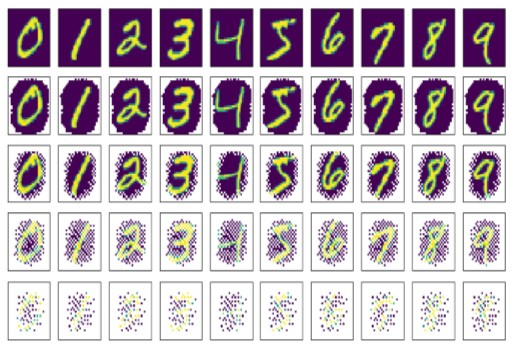
\includegraphics[scale = 1.0]{img/mnist reduced.jpg}
		\label{mi}
        \caption{Example of feature selection on MNIST dataset}
\end{figure}

\paragraph{Optimal Brain Surgeon algorithm (OBS).} This is another pruning algorithm, which focuses on the removal of a single connection, and it rescales all the weights in the network.

Consider a network which is trained to a local minimum in error $E$, i.e. the output of the back-propagation algorithm is $\min_{w \in \mathbb{R}^n} E(w)$. Then, we have that:

$$
\delta E = \bigleft( \frac{\partial E}{\partial w} \bigright)^T \cdot \delta w + \frac{1}{2} \delta w^T \cdot H \cdot \delta w + O(||\delta w||^3)
$$
, where:

\begin{itemize}
    \item $\delta E = E(w) - E(w + \delta w)$;
    \item $\bigleft( \frac{\partial E}{\partial w} \bigright)^T \cdot \delta w \approx 0$, because we're choosing the minimum $w$, so the partial derivative of $E$ is 0;
    \item $  O(||\delta w||^3) \approx 0$;
    \item $H = \frac{\partial^2 E}{\partial w^2}$ represents the Hessian matrix, containing all the second derivative information.
\end{itemize}

In this sense, removing a single connection means setting one of the weights, which will be called $w_q$, to 0, so as to minimize the increase in error $\delta E$. Thus, eliminating $w_q$ can be expressed as:

$$
\delta w_q + w_q = 0
$$

or 

$$
e_q^T \cdot \delta w + w_q = 0
$$
, where $e_q$ is the unit vector in the weight space corresponding to $w_q$, i.e. $e_q = [0 .. 1 .. 0]$, where the 1 is in position $q$. The final goal is then to solve the following constrained optimization problem:

$$
\min_q \min_{\delta w} \frac{1}{2} \delta w^T \cdot H \cdot \delta w \qquad \text{such that } e_q^T \cdot \delta w + w_q = 0
$$

We can transform this constrained problem into an unconstrained one using the \textbf{Lagrangian} (and by adding some more variables):

$$
L = \frac{1}{2} \delta w^T \cdot H \cdot \delta w + \lambda (e_q^T \cdot \delta w + w_q)
$$
, where $\lambda$ is the (undetermine) Lagrange multiplier. The goal now is to find the stationary points of $L$, i.e. points in which all its partial derivatives vanish. Tanking the partial derivatives and setting them to zero we obtain:

$$
\frac{\partial L}{\partial \delta w} = H \delta W + \lambda e_q = 0
$$

and

$$
\frac{\partial L}{\partial \lambda} = e_q^T \delta w + w_q = 0
$$

, from which we obtain that:

$$
\delta w = - \frac{w_q}{(H^{-1})_{qq}} H^{-1} \cdot e_q
$$

and 

$$
L = \frac{1}{2} \frac{w_q^2}{(H^{-1})_{qq}}
$$

, where $H^{-1}$ represents the inverse of the Hessian matrix, which is very computational demanding.

Finally, the algorithm proceeds as follows:

\begin{enumerate}
    \item Train a reasonably large network to minimum error;
    \item Compute $H^{-1}$;
    \item Find the $q$ that gives the smallest $L = \frac{1}{2} \frac{w_q^2}{(H^{-1})_{qq}}$. If this candidate error increase is much smaller than $E$, then the $q$-th weight should be deleted, and we proceed to step 4., otherwise, go to step 5.;
    \item Use the $q$ from step 3. to update all the weights $\delta w = - \frac{w_q}{(H^{-1})_{qq}} H^{-1} \cdot e_q$, and go to step 2.;
    \item No more weights can be deleted without large increases in $E$, so at this point we can re-train the network.
\end{enumerate}

There are some differences between the two pruning algorithms we considered:

\begin{itemize}
    \item In OBS we update all the weights;
    \item In OBS we assume that $O(||\delta w||^3) \approx 0$ and $\bigleft( \frac{\partial E}{\partial w} \bigright)^T \cdot \delta w \approx 0$;
    \item In OBS we assume that the network converges to the minimum;
    \item OBS algorithm is less efficient than Pelillo's.
\end{itemize}


\section{Deep Neural Networks}
The \textbf{philosophy} on which \textbf{Deep Learning} relies is to provide a new method for selecting and extracting the features that are provided as input to a classifier, by exploiting the data of the training set. 

More specifically, instead of selecting manually good features and then using them to feed a classifier, Deep Neural Networks learn from the data a \textbf{feature hierarchy} from the initial pixel image in order to obtain a \textbf{classifier}: each layer extracts features from the output of the previous layer, and finally the training phase involves all the layers, jointly.
\image{img/deep_learning}{Example of deep learning process.}{0.75}

As we can see, each layer of the pipeline learns to extract features from the image/video/pixels (in general, from the data we have), and the \textbf{deeper} the layer is, the \textbf{more abstract} the extracted features are.

\subsection{Shallow vs Deep Networks} \textbf{Shallow architectures} are \textbf{inefficient} at \textbf{representing deep functions}, since they are characterized by a limited number of hidden layers. A shallow network with a large single hidden layer can fit any function (i.e. it is a universal approximator), but on the other hand this increases significantly the number of parameters. 

A \textbf{deep network} can \textbf{fit} functions \textbf{better} with less parameters than a shallow network, increasing the number of hidden layers but decreasing the number of required parameters. Deep networks try to simulate the brain's behavior, in which the electric signals propagate across different layers.
\image{img/shallow_vs_deep}{Shallow vs Deep Networks.}{0.78}

Another important aspect to notice is the \textbf{improvement} in \textbf{performance} with the presence of more data.
\image{img/performances}{Performances improves with more data.}{0.6}
As we can see, in the case of basic ML algorithm after a certain amount of data the performance does not increase anymore: in SVM's, for example, this phenomenon happens since the decision boundary obtained by the model only depends on the support vectors, so increasing the size of the training set does not change the accuracy.

The \textbf{usage} of deep networks is not a \textbf{recent} idea (indeed, these networks are fairly old), but it has been made possible only nowadays thanks to the fact that we have \textbf{more data} and \textbf{more computing power}. In particular, the advances in the field of \textbf{GPUs} have made using deep networks way more feasible than before.

\paragraph{Image classification.} The \textbf{image classification} problem consists in predicting a single label (or a probability distribution over all the possible labels to indicate our confidence, as per the following example) for a given image. Images are 3-dimensional arrays of integers from 0 to 255 of size Width x Height x 3. The 3 represents the three color channels Red, Green and Blue.
\image{img/image_classification}{Image classification example.}{0.5}
In image classification, the most important \textbf{challenges} are the following ones:

\image{img/challenges}{Challenges in image classification.}{0.95}
In order to face these challenges, what we need is a data-driven approach in which we have thousands of categories and hundreds of thousand of images for each category.\\
As it is possible to understand, there's a difference between \textbf{traditional approaches} and \textbf{deep learning}. Indeed, in the first one we extract \textbf{meaningful features} from images through a \textbf{manual} process, while in the second case everything happens \textbf{automatically} thanks to a sequence of \textbf{layers} in which the final ones are useful for classification.

\paragraph{Inspiration from biology.} As we introduced before, functioning of Deep Neural Networks is highly inspired from biology, and in particular the architecture resembles the one in the visual cortex of the brain. Indeed, biological vision is hierarchically organized, and the basic component of this hierarchy is the \textbf{retina}. The cells of the retina are arrayed in discrete layers, with the \textbf{photoreceptors} at the top of them that are divided into:

\begin{itemize}
    \item \textbf{Rods}, which are sensitive to the intensity of the light and to movements;
    \item \textbf{Cones}, which are sensitive to colors.
\end{itemize}

We define \textbf{receptive field} the region of the visual field in which light stimuli evoke responses of a given neuron. In terms of Deep Networks, this makes a distinction between \textbf{fully connected Neural Networks}, in which each neuron is connected to all the neurons of the previous layer, and \textbf{sparsely connected Neural Networks}, in which each neuron is characterized by a corresponding \textbf{receptive field}, i.e. it is connected only to a subset of neurons of the previous layer.

The \textbf{take-home} message of this digression is that the \textbf{visual system} is a \textbf{hierarchy} of \textbf{features detectors}.

\paragraph{The Neocognitron (1980).} The first example example of self-trained network for feature learning was the \textbf{Neocognitron}, introduced in 1980.

\subsection{Convolution}
The \textbf{convolution} is a mathematical operation that takes as input an \textbf{image}, i.e. an array of pixels, and a 3x3 array of numbers (called \textbf{convolution filter}), and applies the 3x3 array in a certain portion of the image, and computes the summation of the products between the pixels of the image and the one in the filter. 

\begin{figure}[h!]
		\centering
        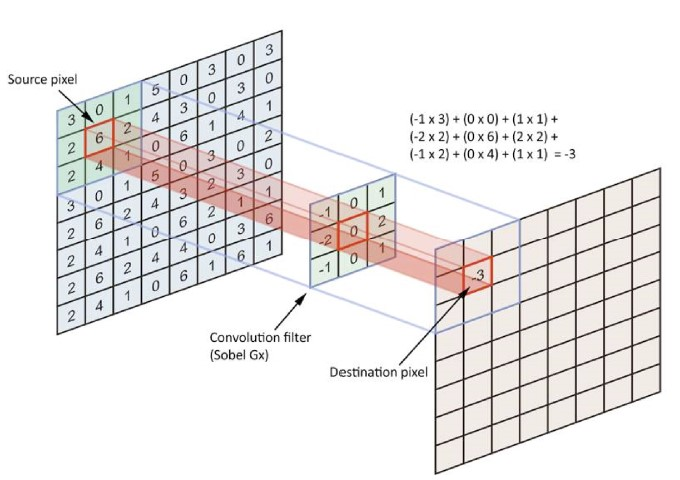
\includegraphics[scale = 1.5]{img/convolution.jpg}
		\label{mi}
        \caption{Example of convolution}
\end{figure}

Notice that there exist many type of filters, which differ for their values.

\begin{figure}[h!]
		\centering
        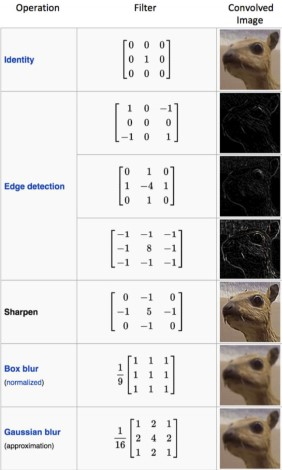
\includegraphics[scale = 1.5]{img/filters.jpg}
		\label{mi}
        \caption{Types of filters}
\end{figure}

\subsubsection{Stride and Padding}

The \textbf{stride} quantity denotes how many steps we're moving in each step of convolution, and the default value is 1. In order to maintain the dimension of the output the same as the one of the input, we use \textbf{padding}, which is the process of adding 0s to the input matrix symmetrically.

\begin{figure}[h!]
		\centering
        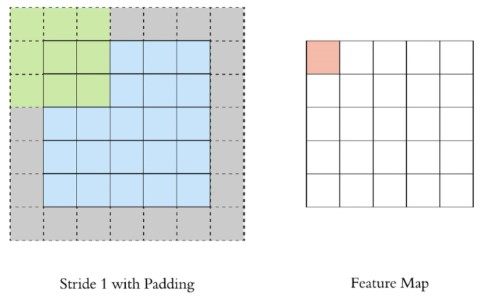
\includegraphics[scale = 1.5]{img/stride and padding.jpg}
		\label{mi}
        \caption{Stride $= 1$ with padding $ = 1$}
\end{figure}

In this sense, \textbf{stride} and \textbf{padding} can be used to \textbf{adjust} the \textbf{dimensionality} of the \textbf{data} effectively.

\subsubsection{Multiple channels}

In the case in which the convolution is applied to an image with multiple channels, we can use a different filter for each channel, and then combine the results into a single output matrix.

\begin{figure}[h!]
		\centering
        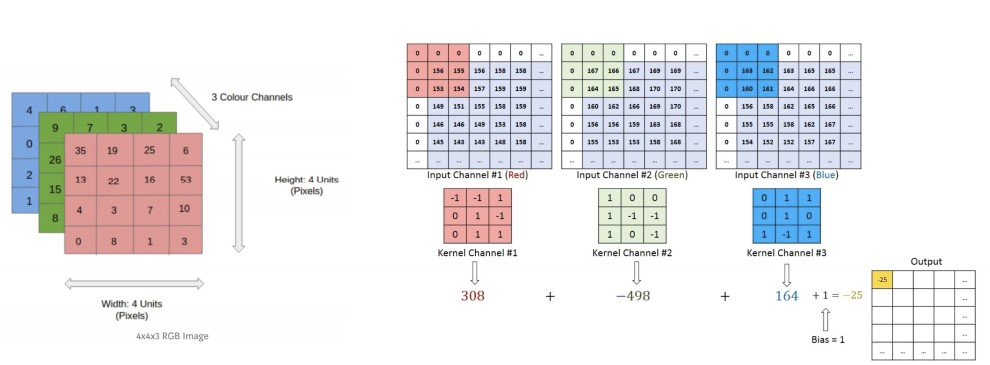
\includegraphics[scale = 1.5]{img/convolution with multiple channes.jpg}
		\label{mi}
        \caption{Example of convolution of an image with multiple channels}
\end{figure}

\subsubsection{Gaussian filter}

A very famous filter used in convolution is the Gaussian filter, which basically computes a weighted average of the pixels of the image, where the weights are proportional to the distance with the central pixel.

\begin{figure}[h!]
		\centering
        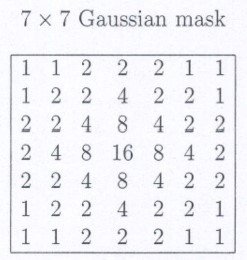
\includegraphics[scale = 1.5]{img/gaussian filter.jpg}
		\label{mi}
        \caption{Example of 7x7 Gaussian filter}
\end{figure}

The result of applying a Gaussian filter to an image is to obtain a \textbf{blurred version} of the image: the larger the filter, the more blurred the output image is.

\subsubsection{Convolution for edge detection and other problems}
An important application of the convolution operation is \textbf{edge detection}, i.e. the problem of determining the contour of an object.

\begin{figure}[h!]
		\centering
        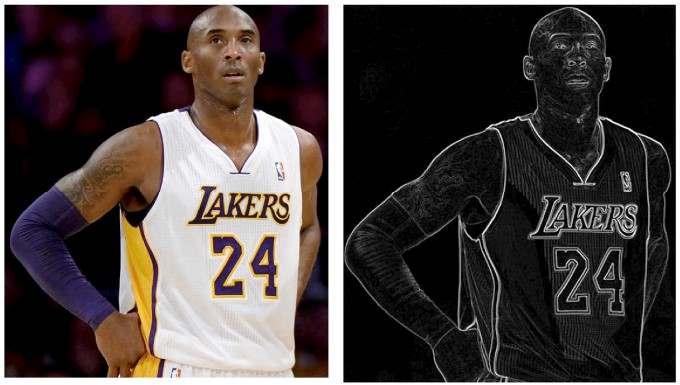
\includegraphics[scale = 1.5]{img/edge detection.jpg}
		\label{mi}
        \caption{Edge detection problem}
\end{figure}

Some of the most famous filters that are used in edge detection are \textit{Roberts operator}, \textit{Sobel operator} and \textit{Prewitt operator}. Other filters are used for different tasks, e.g. \textit{HoG} is used for the problem of \textit{pedestrian recognition} etc..

\subsection{Convolutional Neural Networks (CNNs)} 
\subsubsection{Fully-connected and sparsely-connected networks}
A neural network can be defined as a \textbf{fully-connected network} or a \textbf{locally-connected network}. In a fully-connected network, each neuron of each layer is connected to every neuron in the previous one, and each connection has its own weight. In this sense, the number of parameters is huge.

Conversely, in a locally-connected layer, each neuron is only connected to a \textbf{few nearby neurons} in the previous layer, and the same set of weights (and local connection layout) is used for each neuron. The typical use case for locally-connected layers is for image data where, as required, the \textbf{features} are \textbf{local} (e.g. a "nose" consists of a set of nearby pixels, which are not spread across the whole image), or in general in applications where the local connections capture local dependencies. The smaller number of connections and weights makes local-connected layers \textbf{relatively cheap} in terms of memory and computing power needed.
\image{img/fully_local}{Fully vs local-connected networks.}{0.75}

\subsubsection{Weight sharing}

Before providing the definition of \textbf{CNN}, we now define the concept of \textbf{weight sharing}. This concept is based on the following reasonable assumption: if one feature is useful to compute at some spatial position $(x_1, y_1)$, then it should be useful to compute at a different position $(x_2, y_2)$. In this way we can dramatically reduce the number of parameters.

\begin{figure}[h!]
		\centering
        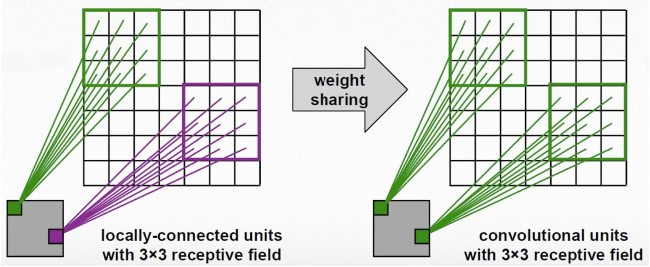
\includegraphics[scale = 1.5]{img/weight sharing.jpg}
		\label{mi}
        \caption{Weight sharing operation}
\end{figure}

As we can see, in the first case we have neurons detecting different features (i.e. different weights in the receptive fields), while in the second case the two neurons have the same weights in the corresponding receptive fields, so they're detecting the presence of the same feature in different portions of the image. Note that while in the traditional convolution operation the weights are applied directly to the pixels of the image, in this case they become the weights of the connections of the receptive fields. 

\subsubsection{Definition of CNN}
A \textbf{Convolutional Neural Network (CNN)} is a \textbf{multi-layer feed-forward neural network} characterized by \textbf{local connectivity} (i.e. neurons with the correspondent receptive field) and \textbf{weights} that are \textbf{shared} across spatial positions. Normally, \textbf{several filters} are \textbf{packed} together and \textbf{learned automatically} during training.
\image{img/trainableFilters}{Using Several Trainable Filters.}{0.75}

\paragraph{Pooling.}\textbf{Pooling} is a way to \textbf{simplify} the network architecture, by downsampling the \textbf{number of neurons} resulting from the filtering operations. An example of pooling technique is the \textbf{max pooling}, in which the \textbf{image} is \textbf{partitioned} in small squares and for each square the pixel with \textbf{maximum value} is taken.
\image{img/max_pooling}{Max Pooling.}{0.6}
As we can see in the next image, a \textbf{Deep Convolutional Neural Network} is a \textbf{combination} of \textbf{feature extraction} and \textbf{classification processes}:

\begin{itemize}
    \item The \textbf{input} of the network is represented by an \textbf{image};
    \item The \textbf{input layer} is followed by some \textbf{locally-connected layers} that \textbf{extract features} from the image. As we can see, this feature extraction phase is mainly composed of \textit{convolution} and \textit{subsampling} operations;
    \item Finally, a \textbf{fully-connected layer} provides the \textbf{classification} of the input image.
\end{itemize}

\image{img/extraction_and_classification}{Combining Feature Extraction and Classification.}{0.7}

\subsection{AlexNet (2012)} 
The first example of Deep Convolutional Neural Network we examine is the \textbf{AlexNet}. This architecture was developed in 2012 for solving the problem of \textbf{image classification}, and it was trained using the \textit{ImageNet} dataset, comprising 1,000 categories, 1.2M training images and 150k test images. The results were astonishing, since the error was reduced by 22\% in only 3 years.

More specifically, this architecture is not so different from the one of the \textit{Neocognitron}, or from the one proposed by LeCun in 1998, but this was much larger. AlexNet is composed of \textbf{8 layers} as per the following schema:
\imageb{img/alexNetLayers}{0.18}
The first thing we can notice are that:

\begin{itemize}
    \item The \textbf{input} is given by an \textbf{image};
    \item The \textbf{first 5 layers} are used for \textbf{extracting features} for the classification phase: as we can see, we have a combinations of \textit{convolution} and \textit{pooling} operations;
    \item \textbf{Layer 6 and 7} provide the \textbf{classification} of the input: as we can see, in this case we exploit fully connected layers;
    \item The \textbf{output layer} is represented by a \textbf{Softmax} function, which provides a probability distribution of the classes of the input image.
\end{itemize}

\image{img/alexNet}{AlexNet architecture.}{0.8}

Diving deeper into these layers' characteristics, we can notice that:
\begin{itemize}
	\item \textbf{1st layer:} we have 96 kernels of size $(11 \times 11 \times 3)$, which are applied to the input image: the results is then convolved (stride = 4) and pooled. Notice that the output of the first layer has not a width of 96, and this is because it was splitted into two different outputs, each with width equal to 48. By looking at the top-9 patches for one filter we can observe that the neurons are very sensitive for colors and geometric forms, so they're very simple;
	\item \textbf{2nd layer:} we have 256 kernels of size $(5 \times 5 \times 48)$, which are then normalized and pooled. Notice the 256 kernels are given by two blocks of 128 kernels. Here the neurons distinguish more abstract features, and this process continues as we go deeper in the Deep Network;
	\item \textbf{3rd layer:} we have 384 kernels of size $(3 \times 3 \times 256)$;
	\item \textbf{4th layer:} we have 384 kernels of size $(3 \times 3 \times 192)$;
	\item \textbf{5th layer:} we have 256 kernels of size $(3 \times 3 \times 192)$;
	\item \textbf{6th layer:} we have a fully connected layer with 4096 neurons;
	\item \textbf{7th layer:} we have a fully connected layer with 4096 neurons;
	\item \textbf{8th layer:} we have a 1000-way \textbf{SoftMax} output layer, i.e. 1 output for each of the possible classes, since it provides a probability distribution.
\end{itemize}
While training the network, two independent GPUs run in parallel, in order to speedup the training process. This is the reason why the output of the first layer was splitted. 

The last \textit{SoftMax} layer gives as output:
$$y_i = \frac{e^{z_i}}{\sum_j e^{z_j}}$$
, where $z_i$ represents the output of the network and it is defined as:

$$
z_i = w_i^T \cdot x
$$

\begin{figure}[h!]
		\centering
        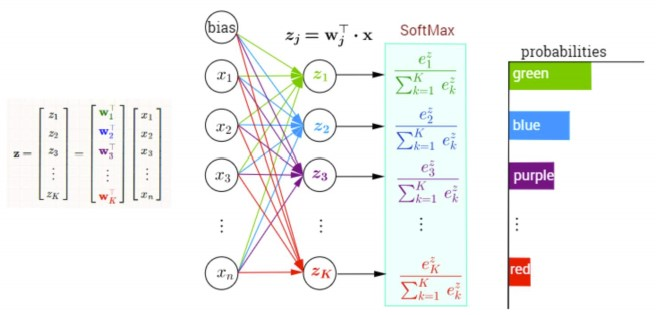
\includegraphics[scale = 1.5]{img/softmax.jpg}
		\label{mi}
        \caption{Output of the SoftMax function}
\end{figure}

Since the output of the SoftMax is a probability distribution over all the possible classes of the training set, we can compute the \textbf{Cross-entropy loss} between the actual output and the desired one, in order to measure the quality of the model.

\subsection{ReLU} \textbf{ReLU} is an acronym that stands for \textit{Rectified Linear Unit}. ReLUs are used to solve the \textbf{problem} that \textbf{sigmoid activation} takes only values in $(0,1)$. While propagating the gradient back to the initial layers, it tends to get closer and closer to $0$ (this phenomenon is called \textit{vanishing gradient}, and it intensifies when the number of layers is high). From a practical perspective, this slows down the training procedure of the initial layers of the network. Indeed, with sigmoid the gradient will be close to 0 and the algorithm won't learn. In order to speed up the learning phase, ReLU is used.
\image{img/relu}{Comparison between sigmoid and ReLU functions.}{0.8}
It is also possible to notice that ReLU reaches the \textbf{same results as sigmoid}, but \textbf{much faster}. In the following image, the solid line represents the convergence of a 4 layer CNN with ReLUs, while the dashed line represents an equivalent network with $tanh$ neurons. It can be noticed that the CNN with \textbf{ReLUs converges six times faster}.
\image{img/relu2}{Convergence of ReLU neurons.}{0.4}

\subsection{Mini-batch Stochastic Gradient Descent} 
We recall that in the back-propagation algorithm we can have either the \textbf{on-line} implementation or the \textbf{off-line} one: in the first one, the weights are updated at any presentation of an example of the training set, while in the second one the gradient is computed exactly. We indicated the \textbf{stochastic gradient descent} as a possible compromise between the two approaches, now we introduce the \textbf{mini-batch stochastic gradient descent}, which is defined as follows:

\begin{enumerate}
	\item Sample a batch of data (the dimension is an hyperparameter to choose), i.e. a subset of the training set;
	\item Perform the forward pass and compute the loss;
	\item Perform the backward pass to compute the gradients;
	\item Update the weights using the gradient (by minimizing the loss).
\end{enumerate} 

Notice that, like in stochastic gradient descent, the use of random samples helps in finding global minima.

\subsection{Data augmentation}
The easiest and most common method to \textbf{reduce overfitting} on image data is to \textbf{artificially enlarge} the \textbf{dataset} using \textbf{label-preserving transformations}. This technique is used to make the dataset more robust. \textbf{AlexNet} uses two forms of \textbf{data augmentation}:
\begin{itemize}
	\item The first form consists in \textbf{generating image translations} and \textbf{horizontal reflections} (translations, scaling or rotations of the images);
	\item The second form consists in \textbf{altering the intensities} of the \textbf{RGB channels} of the \textbf{training images} (introduce random noise inside the images). 
\end{itemize}

\image{img/dataAugmentationBoys}{Data augmentation: translation, reflection, scaling, rotation, RGB noise.}{0.35}

\subsection{Dropout} This technique is exploited in order to have a network with \textbf{more generalization power}, and it consists on \textbf{randomly dropping out some neurons} during the back-propagation algorithm, by setting to 0 the output of that neuron with probability $0.5$. The neurons which are \textit{"dropped out"} in this way do not contribute to the forward pass and do not participate in back-propagation. Every time an input is presented, the neural network samples a different architecture, but all these architectures share weights.\\
Dropout reduces complex co-adaptations of neurons, and it forces the network to find different "roads" in order to produce the outputs, resulting in a more robust network.
\image{img/dropout}{Dropout results}{0.55}

\subsection{Feature analysis}
A well trained Deep Convolutional Neural Network is an excellent \textbf{feature extractor}: in particular, the idea is to chop the network at a desired layer and use the output as a feature representation to train a SVM on some other dataset. Here we show some results.

\begin{figure}[h!]
		\centering
        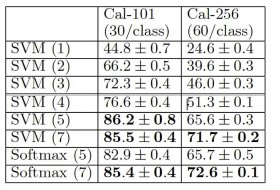
\includegraphics[scale = 2.0]{img/feature extraction.jpg}
		\label{mi}
        \caption{Results using CNN's as feature extractors}
\end{figure}

The parenthesis indicates the layer at which the output is taken: as we can see, the accuracy of the classifier increases as we choose features from more layers, underlying the property of CNN's of learning more and more accurate features as the number of layers grow.

\subsection{CNN's in computer vision tasks}
After 2012, many CV tasks were addressed using CNN's, for example:

\begin{itemize}
    \item \textbf{Semantic segmentation}: in this case the input is an image, and each pixel is classified with a label;
    \item \textbf{Classification and localization}: in this case we assume that the input image contains a single prominent object, and the output consists of single label of the object (standard classification) together with the position of the object;
    \item \textbf{Object detection}: in this case we detect all the objects in an image, where the number is not known in advance;
    \item \textbf{Instance segmentation}: this problem represents a variation of the image segmentation problem, and it consists of labeling each pixel differentiating between objects having the same label.
\end{itemize}

\begin{figure}[h!]
		\centering
        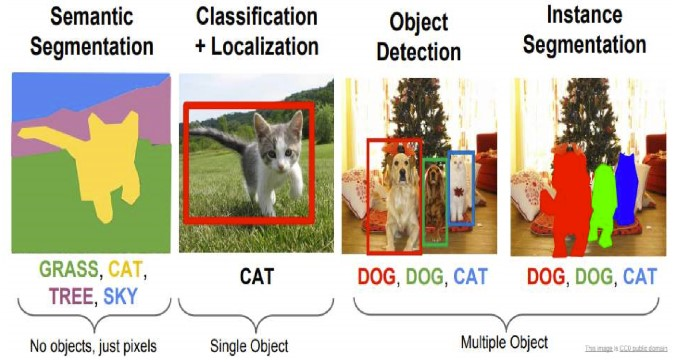
\includegraphics[scale = 1.5]{img/cv tasks.jpg}
		\label{mi}
        \caption{Computer vision problems}
\end{figure}

In general, the adoption of CNN's for solving such problems is having a huge impact in the results.

\subsection{Recurrent Neural Networks}
If we consider the problem of \textbf{image captioning}, i.e. of providing a textual description of the content of an image, it is clear that the usage of a \textbf{feed-forward neural network} does not help in this case, since the output depends on the input. For this reason, we have to exploit \textbf{recurrent neural networks}.

\begin{figure}[h!]
		\centering
        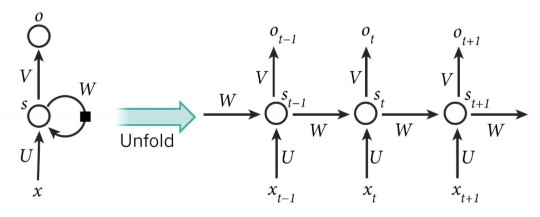
\includegraphics[scale = 1.5]{img/rnn.jpg}
		\label{mi}
        \caption{Recurrent neural network}
\end{figure}

The image shows the unfolding of the simplest recurrent NN, i.e. the one composed of a single hidden layer. Notice that this architecture is different from a feed-forward NN for two main reasons:

\begin{itemize}
    \item We do not know in advance the number of layers;
    \item In a feed-forward NN we have different weights between the layers, while in this case we only have 1 batch of weights for each connection.
\end{itemize}

If we denote with $W_{xh}$ the weights between the input vector $x$ and the RNN, with $W_{hh}$ the weights of the RNN and with $W_{hy}$ the weights between the RNN and the output vector, then:

$$
h_t = \text{tanh} (W_{hh} h_{t-1} + W_{xh} x_t)
$$

and 

$$
y_t = W_{hy} h_t
$$
, where $h_t$ represents the output of the hidden layer at time $t$.

We can have many types of RNN, as shown in the following image.

\begin{figure}[h!]
		\centering
        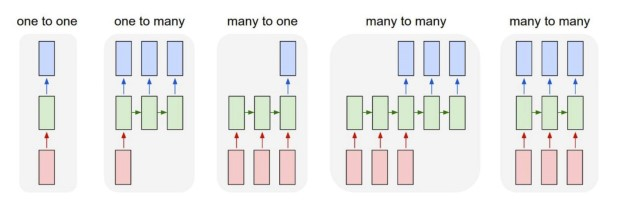
\includegraphics[scale = 1.5]{img/rnn2.jpg}
		\label{mi}
        \caption{Recurrent neural network}
\end{figure}

\begin{itemize}
    \item The \textbf{one-to-many} RNN is used for solving the \textbf{image captioning} problem;
    \item The \textbf{many-to-one} RNN is used for solving the \textbf{sentiment classification} problem (i.e., given a sequence of words, provide the sentiment);
    \item The \textbf{many-to-many} RNN is used for solving the \textbf{machine translation} problem (i.e., given a sequence of words, translating it into another sequence of words). The many-to-many is also used for \textbf{video classification}.
\end{itemize}

\subsubsection{Character-level Language Model}
An example of application of RNN is the character-level language model, in which the goal is to predict the following letter.

\begin{figure}[h!]
		\centering
        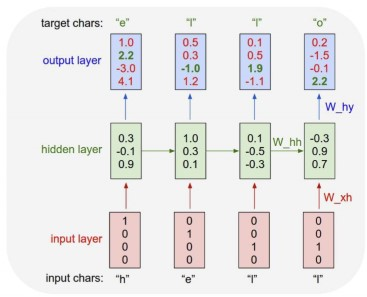
\includegraphics[scale = 1.5]{img/example rnn1.jpg}
		\label{mi}
        \caption{Character-level LM: training}
\end{figure}

As we can see, at test time the predictions at time $t$ are used for the predictions at time $t+1$.

\begin{figure}[h!]
		\centering
        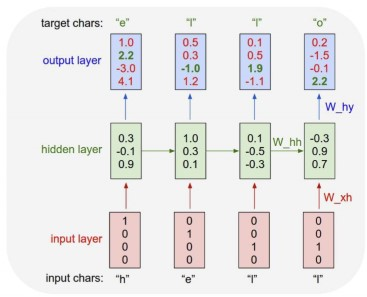
\includegraphics[scale = 1.5]{img/example rnn1.jpg}
		\label{mi}
        \caption{Character-level LM: test}
\end{figure}

However, one possible problems when dealing with RNN is the \textbf{vanishing gradient problem}, so a possible solution is to perform a \textbf{truncated back-propagation}: in this way, the error is backpropagated for a smaller number of steps.

\subsubsection{Image captioning}
We focus now on the image captioning problem: the idea here is to exploit a CNN (in this case AlexNet) to extract the features of an image, and then use these features for training a RNN which can solve the problem.

$$
\text{Image} \to \text{CNN} \to \text{RNN}
$$

\begin{figure}[h!]
		\centering
        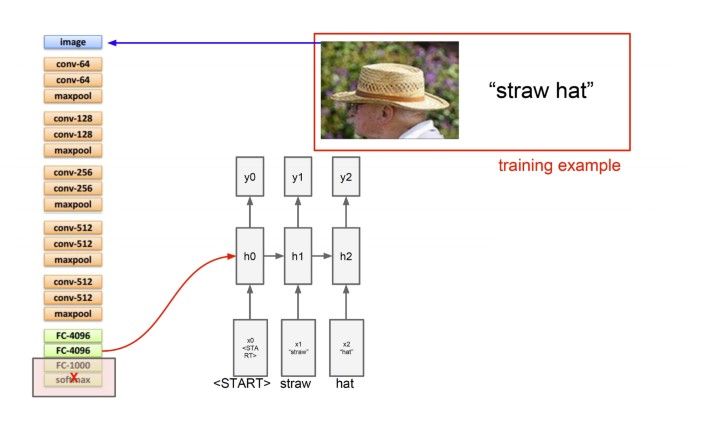
\includegraphics[scale = 1.5]{img/image captioning 1.jpg}
		\label{mi}
        \caption{Image captioning: training}
\end{figure}

As we can see, the last two layers are deleted, since we do not care about the actual classification of the image, but only on the feature the CNN extracted. Finally, the features are provided as input to the RNN, which returns the caption of the image. 

\begin{figure}[h!]
		\centering
        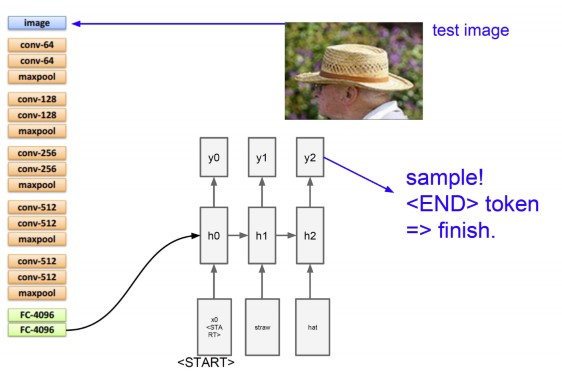
\includegraphics[scale = 1.5]{img/image captioning 2.jpg}
		\label{mi}
        \caption{Image captioning: test}
\end{figure}

At test time, an image without caption is provided as input to the CNN, the features are extracted, and then the RNN is used to provide the caption of the image.

\subsection{Some problems of CNN}
It was showed in several papers how adding some noise bring the Deep Neural Network to misclassify the input image, and this inspired a very important branch of ML, called \textbf{adversarial ML}.

\section{Statistical Learning Theory}
STL mainly deals with \textbf{supervised learning} problems: given an input (feature) space $\mathcal{X}$ and an output (label) space $\mathcal{Y}$ (typically $\mathcal{Y} = \{ +1, -1 \}$), the goal is to estimate a functional relationship between the input and output space:

$$
f: \mathcal{X} \xrightarrow{} \mathcal{Y}
$$

Usually, $f$ is called \textbf{classifier}, so a \textbf{classification algorithm} is a procedure that takes the training data ($(X_1, Y_1), .., (X_n, Y_n) \in \mathcal{X} \times \mathcal{Y}$) as input, and provides the classifier $f$ as output.

\subsection{Assumptions}
Moreover, SLT makes the following \textbf{assumptions}:

\begin{enumerate}
    \item There exists a joint probability distribution $P$ among $\mathcal{X} \times \mathcal{Y}$, which is usually not known;
    \item The training examples $(X_i, Y_i)$ are sampled i.i.d. from $P$.
\end{enumerate}

In particular, 

\begin{itemize}
    \item In STL, no assumptions are made on $P$, whereas in \textit{statistical inference} the data are assumed to follow a certain distribution;
    \item The distribution of $P$ is unknown at learning time;
    \item Non-deterministic labels due to label noise or overlapping classes;
    \item The distribution of $P$ is fixed, both during training and testing.
\end{itemize}

\subsection{Losses and risks}
Clearly, we need to have some measure of how good a function $f$ is when used as a classifier, so a \textbf{loss function} measures the "cost" of classifying instance $x \in \mathcal{X}$ as $y \in \mathcal{Y}$. 

In this sense, the simplest loss function is the \textbf{0-1 loss}, which is defined as:

$$
l(X,Y,f(X)) = \begin{cases}
    1 \qquad \text{if } f(X) \neq Y \\
    0 \qquad \text{otherwise}
\end{cases}
$$

We can define the \textbf{theoretical risk} of a function $f$ the average loss over data points generated according to the underlying distribution $P$:

$$
R(f) := \mathbb{E}(l(X,Y,f(X)))
$$

The \textbf{best classifier} is the one with the smallest risk $R(f)$: among all possible classifiers, the best one is the \textit{Bayes classifier}:

$$
f_{\text{Bayes}} := \begin{cases}
    1 \qquad \text{if } P(Y = 1 | X = x) \geq 0.5 \\
    -1 \qquad \text{otherwise}
\end{cases}
$$

Its idea is to classify the most frequent class. However, in practice it is impossible to directly compute the Bayes classifier, since the underlying distribution $P$ is unknown to the learner, and estimating $P$ from the data usually doesn't work.

Recall: Bayes' theorem says that:

$$
P(h|e) = \frac{P(e|h) P(h)}{P(e)} = \frac{P(e|h) P(h)}{P(e|h) P(h) + P(e|\Bar{h}) P(\Bar{h})}
$$
, where:

\begin{itemize}
    \item $P(h)$ represents the \textbf{prior probability} of hypothesis $h$;
    \item $P(h|e)$ represents the \textbf{posterior probability} of $h$ after the evidence $e$;
    \item $P(e|h)$ represents the \textbf{likelihood} of evidence $e$ on hypothesis $h$.
\end{itemize}

Returning to the classification problem, now the situation is that given:

\begin{itemize}
    \item A set of training data $(X_1, Y_1), .., (X_n, Y_n) \in \mathcal{X} \times \mathcal{Y}$ drawn i.i.d. from an \textit{unknown} distribution $P$;
    \item A loss function,
\end{itemize}

the goal is to determine a function $f: \mathcal{X} \to \mathcal{Y}$ which has a risk $R(f)$ which is as close as possible to the risk of the Bayes classifier. However, we notice that it is impossible to compute the risk of $f$ without knowing $P$..

\subsection{The nearest neighbor (NN) rule} A possible solution for this problem could be represented by the \textbf{nearest neighbor} approach, according to which the label of a data point $x$ is given by the label of the nearest point to $x$. Notice that in this case, no assumptions about the probability distribution of the data is used, since the method only uses information from the training set.

But, how good is the NN rule? It was showed that:

$$
R(f_{\text{Bayes}}) \leq R_{\infty} \leq 2R(f_{\text{Bayes}})
$$
, where $R_{\infty}$ denotes the expected error rate of NN when the sample size tends to infinity. Notice that we cannot say anything stronger about the bounds, since there are probability distributions for which the performance of the NN rule achieves either the upper or lower bound.

There exist some variations to the NN rule, for example the \textbf{$k$-NN} rule, which uses $k$ nearest neighbors and takes the majority vote, or the \textbf{$k_n$-NN rule}, which does the same, but for $k_n$ growing with $n$.

\textbf{Theorem (Stone, 1977)}: if $n \to \infty$ and $k \to \infty$, such that $k/n \to 0$ (i.e. $n$ grows faster than $k$), then for all probability distributions, $R(k_n - \text{NN}) \to R(f_\text{Bayes})$, i.e. the $k_n - \text{NN}$ rule is universally Bayes consistent.

However, all these NN rule have some \textbf{disadvantages}:

\begin{itemize}
    \item Not having a learning phase (\textit{lazy algorithm}), a huge amount of data must be kept in memory;
    \item They are very time demanding.
\end{itemize}

\subsection{The kernel rule}
The idea of \textbf{kernel rules} is that rather than fixing the number of neighbors, to classify a new point $x$ we might consider fixing a distance $h$ and taking a majority vote among the labels of all examples that fall within a distance $h$ of $x$. 

\begin{figure}[h!]
		\centering
        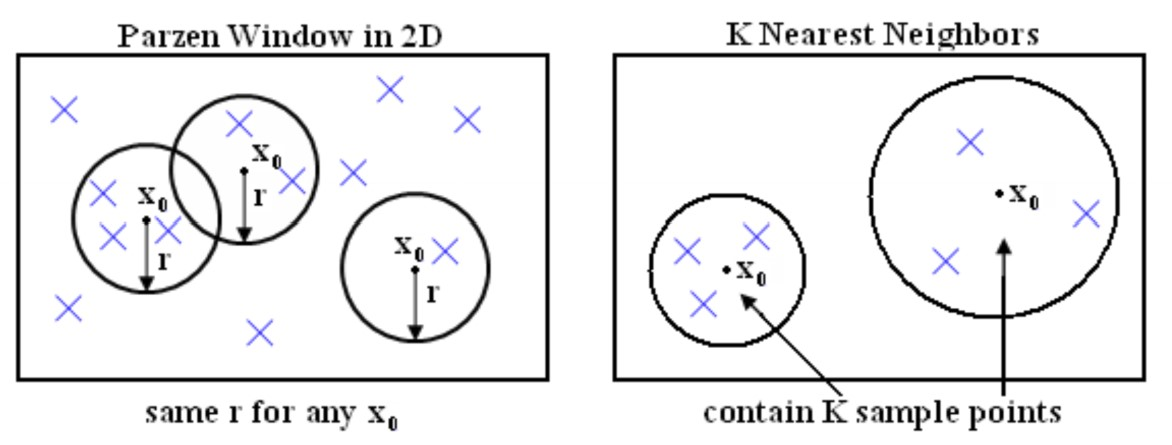
\includegraphics[scale = 1.0]{img/kernel rules.jpg}
		\label{mi}
        \caption{Difference between kernel rules and NN rule}
\end{figure}

Notice that in NN rule, the number of neighbors is fixed, while in kernel rule it depends on the value of $h$. The parameter $h$ is usually called \textbf{smoothing factor} (or \textbf{bandwidth}).

A \textbf{kernel} (a.k.a. \textit{Parzen windows}) is defined as:

$$
K(\Bar{x}) = \begin{cases}
    1 \qquad \text{if } ||\Bar{x}|| \leq 1 \\
    0 \qquad \text{otherwise}
\end{cases}
$$

and we define the vote counts as:

$$
v_n^0(\Bar{x}) = \sum_{i = 1}^n I_{\{ y_i = 0 \}} K \bigleft( \frac{\Bar{x} - \Bar{x}_i}{h} \bigright)
$$

, i.e. the sum of all the elements with label 0 that are within $\Bar{x}$ and $\Bar{x}_i$, and

$$
v_n^1(\Bar{x}) = \sum_{i = 1}^n I_{\{ y_i = 1 \}} K \bigleft( \frac{\Bar{x} - \Bar{x}_i}{h} \bigright)
$$

, i.e. the sum of all the elements with label 1 that are within $\Bar{x}$ and $\Bar{x}_i$.

Then, we assign $x$ to the class 0 if and only if $v_n^0(x) \geq v_n^1(x)$. 

A basic window kernel is represented in Picture \ref{basic kernel}, while Picture \ref{different kernels} shows other possible kernels that can be used.

\begin{figure}[h!]
		\centering
        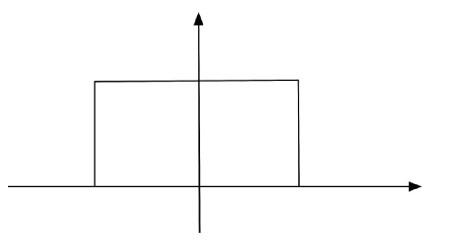
\includegraphics[scale = 1.0]{img/basic window kernel.jpg}
		\label{basic kernel}
        \caption{Basic window kernel}
\end{figure}

\begin{figure}[h!]
		\centering
        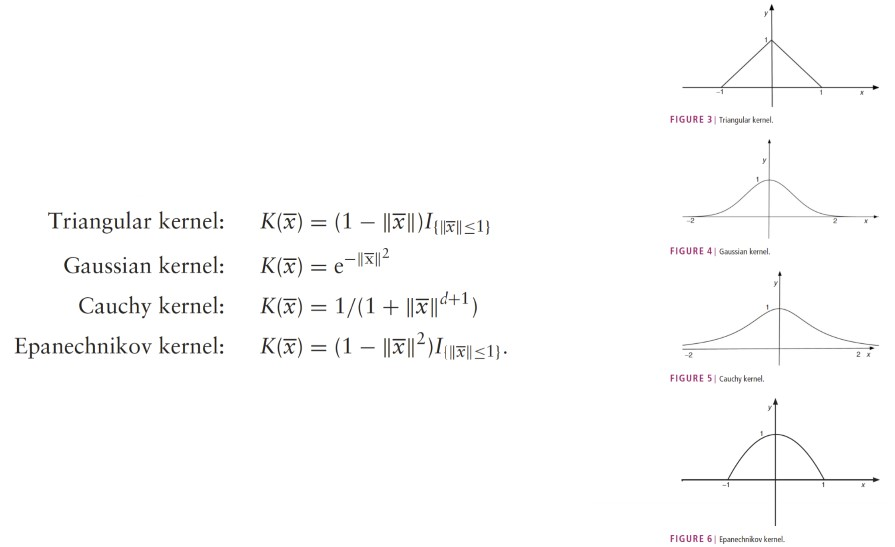
\includegraphics[scale = 1.2]{img/different kernels.jpg}
		\label{different kernels}
        \caption{Other possible kernels}
\end{figure}

\subsection{Empirical Risk Minimization (ERM)}
At the end of 1960's, the \textbf{Empirical Risk Minimization} theory was introduced, and it is based on the following \textbf{principle}: instead of looking for a function which minimizes the true risk $R(f)$, we try to find one which minimizes the \textbf{empirical risk}, i.e. the error the model makes on the training data, which is defined as:

$$
R_{\text{emp}} = \frac{1}{n} \sum_{i = 1}^n l(X_i, Y_i, f(X_i))
$$

Given a training data $(X_1, Y_1), .., (X_n, Y_n) \in \mathcal{X} \times \mathcal{Y}$, a function space $\mathcal{F}$ and a loss function, we define the classifier $f_n$ as:

$$
f_n := \text{arg} \min_{f \in \mathcal{F}} R_{\text{emp}}(f)
$$

, i.e. we choose from $\mathcal{F}$ the function that minimizes the empirical risk. This approach is called the \textbf{empirical risk minimization (ERM)} induction principle, and is motivated from the law of large numbers.

However, we have the issue of how to choose the function space $\mathcal{F}$: a fundamental result in SLT is that the set of rules in $\mathcal{F}$ cannot be too rich, where the richness of $\mathcal{F}$ is measured by its \textbf{VC dimension}.

\subsection{Estimation vs approximation}
Before proceeding, let us introduce a few concepts:
\begin{itemize}
	\item \textbf{Bayes error}: error of the best possible predictor (i.e. the Bayes predictor);
	\item \textbf{Approximation error}: error related to the type of model we are assuming (i.e. related to $\mathcal{F}$). The model may not reflect the nature of the underlying probability distribution. In other words, the approximation error is the minimum generalization error achievable by a predictor in $\mathcal{F}$, and it depends only of $\mathcal{F}$;
	\item \textbf{Estimation error}: error of a predictor belonging to family $\mathcal{F}$. Each predictor in the family will bring an additional error to the approximation error. In other words, the estimation error is the difference between the error of the considered predictor and the error of the predictor, belonging to $\mathcal{F}$, which minimizes the training error (the "best" predictor). The quality of this estimate depends on both the (size of) the training set and on the complexity of the hypothesis class $\mathcal{F}$.
\end{itemize}

Ideally we want to make $R(f_n) - R(f_{Bayes})$ as small as possible, as $n \rightarrow \infty$. Denoting by $f_{\mathcal{ F }}$ the best classifier in $\mathcal{ F }$, the difference can be decomposed as:
$$R \left( f _ { n } \right) - R \left( f _ { B a y e s } \right) = \underbrace{\left( R \left( f _ { n } \right) - R \left( f _ { \mathcal { F } } \right) \right)}_{\text{estimation error}} + \underbrace{\left( R \left( f _ { \mathcal { F } } \right) - R \left( f _ { \text {Bayes} } \right) \right)}_{\text{approximation error}}$$

, where

\begin{itemize}
	\item $R(f_n)$ is the risk of the considered classifier;
	\item $R(f_\mathcal{ F })$ is the risk of the best classifier $f$ on the family $\mathcal{ F }$;
	\item $R \left( f _ { \text {Bayes} } \right)$ is the risk of the best classifier overall (Bayes).
\end{itemize}

\image{img/estimation}{Estimation vs approximation.}{0.35}

According to the complexity of $\mathcal{ F }$ we can have:
\begin{itemize}
	\item \textbf{small complexity} of $\mathcal{ F }$: small estimation error (small \textbf{variance}), large approximation error (large \textbf{bias}), resulting in \textit{underfitting};
	\item \textbf{large complexity} of $\mathcal{ F }$: large estimation error (large \textbf{variance}), small approximation error (small \textbf{bias}), resulting in \textit{overfitting}.
\end{itemize}

The best overall risk is achieved for "moderate" complexity.

\image{img/overunderfitting}{Underfitting vs Overfitting graph}{0.55}
\image{img/modelselection}{Model selection.}{0.8}

\paragraph*{Shattering.} A set of $n$ instances $x_1, \dots, x_n$ from the input space $\mathcal{X}$ is said to be \textit{shattered} by a function class $\mathcal{ F }$ if all the $2^n$ labelings of them can be generated using functions from $\mathcal{ F }$.\\ 
For instance, with $\mathcal{ F }$ as a linear decision functions (straight lines) in the plane, we can have:
\begin{enumerate}[label=(\alph*)]
	\item Any set of 3 non-collinear points shatters $\mathcal{ F }$
	\item No set of 4 points can shatter $\mathcal{ F }$
\end{enumerate}
\imageb{img/shattered}{0.85}

\paragraph*{The Vapnik–Chervonenkis dimension.} The \textbf{VC dimension} of a function class $\mathcal{ F }$, denoted $VC(\mathcal{ F })$, is the largest integer $h$ such that there exists a sample of size $h$ which is shattered by $\mathcal{ F }$. It is a measure of complexity of a function class.\\
If arbitrarily large samples can be shattered, then $VC(\mathcal{ F }) = \infty$.\\
For example:
\begin{itemize}
	\item $\mathcal{ F }$ = linear decision functions in $\mathbb{R}^2 \rightarrow VC(\mathcal{ F }) = 3$
	\item $\mathcal{ F }$ = linear decision functions (hyperplanes) in $\mathbb{R}^n \rightarrow VC(\mathcal{ F }) = n+1$ 
	\item $\mathcal{ F }$ = multi-layer perceptrons with $W$ weights $\rightarrow VC(\mathcal{ F }) = O(W~\log( W))$
	\item $\mathcal{ F }$ = nearest neighbor classifiers $\rightarrow VC(\mathcal{ F }) = \infty$
\end{itemize}


The VC dimension of a classifier depends on the dimension of the space the data points belong to. For instance, if we consider our space to be $\mathbb{R}^2$, then the VC dimension is $3$. As a matter of fact,  $\mathbb{R}^2$ can always shatter any three general position points ("general position" means they do not coincidentally lie on the same line). For instance, consider three points $(0,0)$, $(0,1)$, $(1,0)$. No matter how labels are assigned to them, a line can always separate them. Conversely, let's consider four points $(0,0)$, $(0,1)$, $(1,0)$, $(1,1)$ with label $[+,-,-,+]$, representing the "XOR" function. This function cannot be separated by a line. For $x\in\mathbb{R}$, then the VC dimension is 2 because you cannot separate $+-+$. In general for $x\in\mathbb{R}^d$, the VC dimension for a linear classifier is $d+1$.\\

The \textbf{VC dimension} is usually \textbf{unrelated} to the \textbf{number of free parameters of a model}.\\
For all $f \in \mathcal{ F }$, with probability at least $1-\delta$, we have:
$$
R ( f ) \leq R _ { \mathrm { emp } } ( f ) + \underbrace{\sqrt { \frac { h ( \log ( 2 n / h ) + 1 ) - \log ( \delta / 4 ) } { n } }}_{\text{VC confidence}}
$$
where 

\begin{itemize}
    \item $h=VC(\mathcal{ F })$ is the VC dimension of the family $F$;
    \item $\delta$ is a tolerance parameter;
    \item $n$ is the sample size.
\end{itemize}

We can read this results as:\\

\textit{With probability approaching  1, no matter what the unknown probability distribution, given more and more data, the expected error for the functions that ERM endorses at each stage eventually approaches the minimum value of expected error of the functions in $\mathcal{ F }$ if and only if $\mathcal{ F }$ has finite VC dimension. If VC dimension is equal to $\infty$, like in the KNN case, we have that $R_\text{emp}(f) = 0$ and so $R(f) \leq \infty$ which is meaningless.}\\

Intuitively, since the second term $R_\text{emp}\dots$ is an upper bound, if it is small, $R(f)$ will be small too. This result is fundamental due to the fact that we have no knowledge about $P$, thus we cannot compute $R(f)$, but we can have a \textbf{bound} for it using the second quantity. Indirectly we want to \textbf{reduce the bound} so that at the end the resulting \textbf{risk} is \textbf{minimized}.

\paragraph*{Structural Risk minimization.} It is a general framework for choosing the best classifier. Empirical Risk Minimization only takes care of the \textit{estimation} error (variance) but it is not concerned with the \textbf{approximation error} (bias). The optimal model is found by striking a balance between the empirical risk and the capacity of the function class $\mathcal{ F }$ (ex: the VC dimension).\\
The basic idea of \textit{Structural Risk Minimization} (SRM) is:
\begin{enumerate}
	\item Construct a \textbf{nested} structure for family of function classes $\mathcal{ F }_1 \subset \mathcal{ F }_2 \subset \dots$ with \textbf{non-decreasing VC dimension} $(VC(\mathcal{ F }_1) \leq VC(\mathcal{ F }_2) \leq \dots)$
	\item For \textbf{each class} $\mathcal{ F }_i$, find the solution $f_i$ that \textbf{minimizes} the \textbf{empirical risk}.
	\item Choose the function class $\mathcal{ F }_i$, and the corresponding solution $f_i$ that minimizes the risk bound (= empirical risk + VC confidence) 
\end{enumerate}

Notice that this idea resembles the pruning approach, where we started with a large NN which was trained with back-propagation, and finally reduced. Here the reasoning is the opposite, we start with a small VC dimension and we augment it. 

\image{img/risk_minimization}{Structural risk minimization.}{0.50}
\section{Support Vector Machines (SVMs)}
\subsection{Introduction}
In this section we are going to deal with a very well known \textbf{supervised learning algorithm}, called \textbf{Support Vector Machine}. We will see that it can be written as an intuitive \textbf{optimization problem} and can be easily extended to work very well with non-linear patterns or in \textbf{high dimensional spaces}.\\

SVM belongs to the class of \textbf{discriminative classifiers} since its goal consists on \textbf{learning the class boundary between the two classes} $y$ starting from features $x$. From now, we'll use $y\in\{-1,1\}$ to denote the class labels. In a 2-dimensions feature space the decision boundary is represented by a straight line, while in general the decision boundary is represented by an \textbf{hyperplane}. An example of decision boundaries in a 2-dimensions feature space is represented in Picture \ref{hyperplanes}.

\begin{figure}[h!]
		\centering
		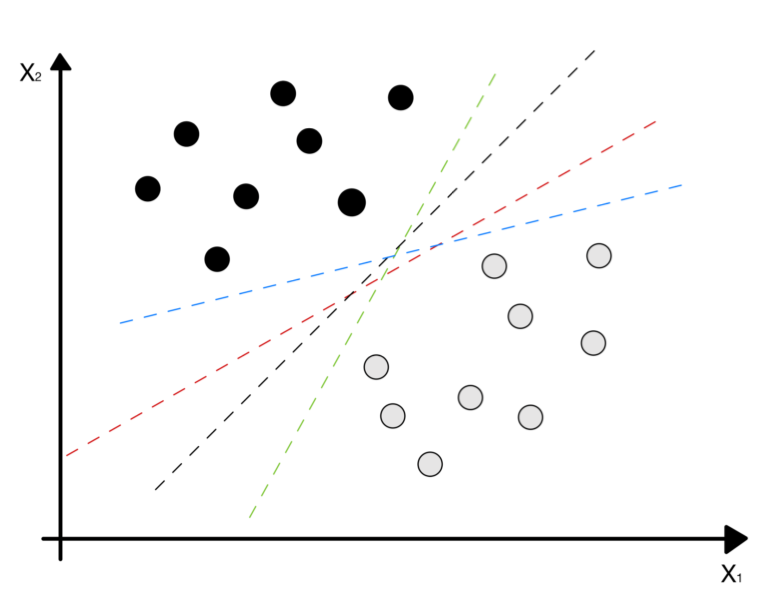
\includegraphics[scale = 1.0]{img/hyperplanes.png}
		\label{hyperplanes}
		\caption{Decision boundaries in a 2-dimensions feature space}
\end{figure}

The data points that are closest to the decision boundary are called \textbf{support vectors}, while the distance between the support vectors along the perpendicular direction to the selected hyperplane is called \textbf{margin}: the hyperplane chosen by SVM is the one that maximize the margin. By choosing this particular hyperplane, the \textbf{misclassification risk} is minimized, since the \textbf{confidence} of the prediction of the model is stronger.

From a mathematical point of view, let's consider a 2-dimension feature space and let's assume labels are such that $y_i \in \{-1, 1\}$. A linear decision boundary $B$ is defined by the equation:
$$
    w^Tx + b = 0
$$
, where $w$ weights the features of $x$, so the objects above $B$ are defined by $w^Tx + b = k'$, where $k' > 0$, while the objects below $B$ are define by $w^Tx  b = k''$, where $k'' < 0$. Let $x_s$ and $x_c$ be the positive and negative support vectors of $B$, we can then rescale $w$ and $b$ such that:

$$
w^Tx_s + b = 1
$$

and 

$$
w^Tx_c + b = -1
$$

Let $d_s$ and $d_c$ be the distances between the support vectors and the decision boundary $B$, then by definition:

$$
d_s = \frac{|w^Tx_s + b|}{||w||} = \frac{|1|}{||w||} = \frac{1}{||w||}
$$

$$
d_c = \frac{|w^Tx_c + b|}{||w||} = \frac{|-1|}{||w||} = \frac{1}{||w||}
$$

Then, the margin $d$ is defined as:

$$
d = d_s + d_c = \frac{2}{||w||}
$$

\begin{figure}[h!]
		\centering
		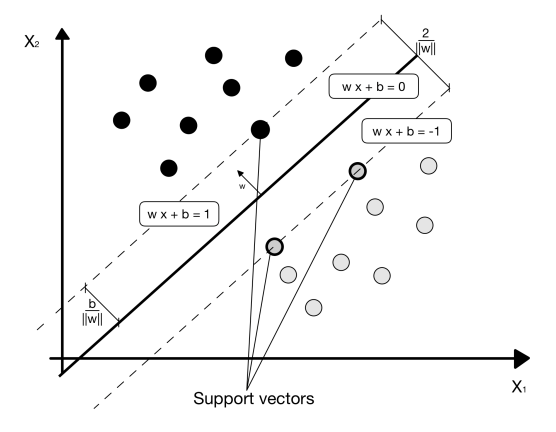
\includegraphics[scale = 1.0]{img/sv.png}
		\label{svm}
		\caption{Geometric representation of SVM}
\end{figure}

Thus, given a training set $L = \{ (x_1, y_1), .., (x_N, y_N) \}$, learning an SVM can be formulated as an optimization problem: indeed, the goal of SVM is to \textbf{maximize} $\frac{2}{||w||_2}$ or, equivalently, \textbf{minimize} $\||w||_2$. Finally, we can describe the SVM (binary) classification problem as:

\begin{equation}\label{eq_svm1}
\begin{aligned}
\max_{w} \quad & \frac{2}{||w||}\\
\textrm{s.t.} \quad & y_{i}(w^Tx_{i}+b) - 1 \geq 0 \quad \forall i = 1,..,N\\ \\
\end{aligned}
\end{equation}

or, equivalently

\begin{equation}\label{eq_svm2}
\begin{aligned}
\min_{w} \quad & \frac{1}{2} ||w||^2\\
\textrm{s.t.} \quad & y_{i}(w^Tx_{i}+b) - 1 \geq 0 \quad \forall i = 1,..,N\\ \\
\end{aligned}
\end{equation}

Since the objective functions in \ref{eq_svm1} and \ref{eq_svm2} are quadratic, and the constraints are linear in $w$ and $b$, this is known to be a \textbf{convex optimization problem}, which means that there exists a unique minimum! This unique minimum corresponds to the \textbf{optimal margin classifier}. 

\subsection{Lagrangian and duality}
\subsubsection{Unconstrained optimization}
Suppose we want to find the maximum of the following 2-dimensions function:

$$
f(x,y) = 1 - x^2 - y^2
$$

From calculus we know that the solution must be found among the points $(x,y)$ where the gradient $\nabla f(x,y)$ vanishes, i.e. in the so-called \textbf{stationary points}:

$$
\frac{\partial f(x,y)}{\partial x} = -2x = 0
$$

and

$$
\frac{\partial f(x,y)}{\partial y} = -2y = 0
$$

In this sense, the solution is given by $x = 0$ and $y = 0$.

\subsubsection{Constrained optimization}
Suppose now that the points $(x,y)$ have to lie on the straight line of equation $x + y = 1$, i.e. we want to solve the following constrained optimization problem:

\begin{equation*}\label{eq_svm2}
\begin{aligned}
\max \quad & 1 - x^2 - y^2\\
\textrm{s.t.} \quad & x + y - 1 = 0\\ \\
\end{aligned}
\end{equation*}

Our goal is now to define a method for transforming the constrained optimization problem into an unconstrained one. To this end, we define a new function $L(x,y,\lambda)$, called the \textbf{Lagrangian} as follows:

$$
L(x,y,\lambda) = 1 - x^2 - y^2 + \lambda(x + y - 1)
$$

, where $\lambda \neq 0$ is called a \textbf{Lagrangian multiplier}, and looks for points $(x,y,\lambda)$ where the gradient $\nabla L$ vanishes. Notice that in $L$ we now have as many new variables as the constraints we have. If we apply this method to example, we get the following system of linear equations:

$$
\frac{\partial L(x,y,\lambda)}{\partial x} = -2x + \lambda = 0
$$

$$
\frac{\partial L(x,y,\lambda)}{\partial y} = -2y + \lambda = 0
$$

$$
\frac{\partial L(x,y,\lambda)}{\partial \lambda} = x + y - 1 = 0
$$

, from which we get the solution $x = y = \frac{1}{2}$

\subsubsection{General case}
More generally, given the following optimization problem:

\begin{equation*}\label{eq_svm2}
\begin{aligned}
\max \quad & f(x)\\
\textrm{s.t.} \quad & g_1(x) \geq 0 .. g_m(x) \geq 0  \\
\textrm{    } \quad & h_1(x) = 0 .. h_n(x) = 0
\end{aligned}
\end{equation*}

, where we have $m$ inequality constraints and $n$ equality constraints, the Lagrangian is defined as:

$$
L(x, \Lambda, M) = f(x) + \sum_{i = 1}^m \lambda_i g_i(x) + \sum_{j = 1}^n \mu_j h_j(x)
$$
, where $\Lambda = (\lambda_1, .., \lambda_m)^T$ and $M = (\mu_1, .., \mu_n)^T$ are vectors of Lagrange multipliers corresponding to inequality and equality constraints, respectively.

In this case we need to impose the conditions $\lambda_i \geq 0$ and $\lambda_i g_i(x) = 0$ for all $i = 1,..,m$

The \textbf{intuition} behind the \textbf{equality constraints} is the following one: at any point $x$ in the constraint surface, $\nabla g(x)$ is normal to the surface, from the properties of the gradient. Then, if $x$ is also a maximizer of $f$, $\nabla f(x)$ must be orthogonal to the surface too (otherwise we could increase the value of $f$ with another point), so we have that:

$$
\nabla f(x) = - \lambda \nabla g(x)
$$

, with $\lambda \neq 0$.

\begin{figure}[h!]
		\centering
		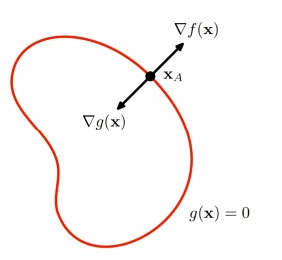
\includegraphics[scale = 1.5]{img/equality constraints intuition.jpg}
		\label{svm}
		\caption{Equality constraints}
\end{figure}

The \textbf{intuition} behind the \textbf{inequality constraints} is the following one. We have two cases:

\begin{itemize}
    \item The solution is in the interior, i.e. $g(x) > 0$: in this case the stationary point condition implies $\nabla f(x) = 0$, which corresponds to the case $\lambda = 0$;
    \item The solution is on the boundary, i.e. $g(x) = 0$: this is analogous to the previous case, but this time the sign of $\lambda$ is crucial: hence $\nabla f(x) = -\lambda \nabla g(x)$, with $\lambda > 0$.
\end{itemize}

For either of these cases we have $\lambda g(x) = 0$

\begin{figure}[h!]
		\centering
		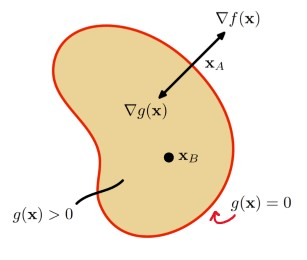
\includegraphics[scale = 1.5]{img/inequality constraints intuition.jpg}
		\label{svm}
		\caption{Inequality constraints}
\end{figure}

Notice that if we want to minimize, rather than maximize, $f(x)$, the Lagrangian multipliers have to be non-positive, or simply change the sign of the corresponding term in the Lagrangian.

\subsubsection{Duality}
Consider the following optimization problem with inequality constraints, called the \textbf{primal}:

\begin{equation*}\label{duality}
\begin{aligned}
\min \quad & f(x)\\
\textrm{s.t.} \quad & g_1(x) \geq 0 .. g_m(x) \geq 0  \\
\end{aligned}
\end{equation*}

with optimal value $p^*$, and consider its Lagrangian:

$$
L(x, \lambda_1, .., \lambda_m) = f(x) - \sum_{i = 1}^m \lambda_i g_i(x)
$$

Notice that the Lagrangian has a minus sign since the problem is a minimization.

Given $\lambda_1, .., \lambda_m \geq 0$, we define the (Lagrangian) \textbf{dual function} as:

$$
\phi(\lambda_1, .., \lambda_m) = \inf_x L(x, \lambda_1, .., \lambda_m)
$$

It's easy to see that $\phi(\lambda_1, .., \lambda_m) \leq p*$, i.e. the optimal value of the previous problem is an upper bound of this second problem.

The problem 

\begin{equation*}\label{eq_svm2}
\begin{aligned}
\max \quad & \phi(\lambda_1, .., \lambda_m)\\
\textrm{s.t.} \quad & \lambda_1, .., \lambda_m \geq 0  \\
\end{aligned}
\end{equation*}

is called the (Lagrangian) \textbf{dual} of problem \ref{duality}.

\paragraph{Weak duality:} if $p^*$ is a solution of the primal and $d^*$ is a solution of its dual, then:

$$
d^* \leq p^*
$$

The quantity $d^* - p^* \leq 0$ is called \textbf{duality gap}.

\paragraph{Strong duality:} if the function $f$ of the primal is convex (and so are all $-g_i$), then

$$
p^* = d^*
$$
, i.e. the solution of the dual (which is simpler) is the same as the solution of the primal.

\paragraph{Wolfe duality:} the \textbf{Wolfe dual} is defined as:

\begin{equation*}\label{eq_svm2}
\begin{aligned}
\max_{x,\Lambda} \quad & L(x,\Lambda)\\
\textrm{s.t.} \quad & \nabla_x L(x,\Lambda) = 0  \\
\textrm{    } \quad & \Lambda \geq 0  \\
\end{aligned}
\end{equation*}

, where $\Lambda = (\lambda_1, .., \lambda_m)$.

Assume that functions $f$ and $-g_i$ are convex (and continuously differentiable): if $x^*$ is a solution of the \textbf{primal problem}, then there exists a \textbf{vector of Lagrangian multipliers} $\Lambda^*$ s.t. $(x^*, \Lambda^*)$ is a \textbf{solution} of the \textbf{Wolfe dual}, and the duality gap is 0.

\subsubsection{Dual representation of SVM}
In order to solve constrained problem 

\begin{equation}\label{eq_svm2}
\begin{aligned}
\min_{w} \quad & \frac{1}{2} ||w||^2\\
\textrm{s.t.} \quad & y_{i}(w^Tx_{i}+b) - 1 \geq 0 \quad \forall i = 1,..,N\\ \\
\end{aligned}
\end{equation}

we introduce the concept of \textbf{Lagrange multipliers}. Using the \textbf{Lagrange} function with $N$ Lagrange multipliers $\Lambda = (\lambda_1,\dots,\lambda_N)$ (one for each constraint) it is possible to rewrite the correspondent optimization problem, with parameters $w$ and $b$, into an identical one but with parameters $(\lambda_1,\dots,\lambda_N)$. Taking advantage of the \textbf{dual representation}, that allows to convert an original min/max problem into another one which is equivalent but with max/min formulation, we can write the \textbf{new optimization problem}as follows:

\begin{equation}
\quad L(w,b,\Lambda) = \frac{1}{2}||w||^2 - \underbrace{\sum_{i = 1}^{N}\lambda_i[y_i(w^Tx_i+b)-1]}_{\text{Sum of constraints}}\\
\end{equation}
, where $\Lambda = (\lambda_1, .., \lambda_N)$ is the vector if Lagrange multipliers.

The goal now is to find a \textbf{function} \textbf{parameterized} only by \textbf{Lagrangian multipliers}. Setting the derivatives of $L(w,b,\Lambda)$ to zero we get:

$$\frac{\partial L(w,b,\Lambda)}{\partial w} = w- \sum_{i = 1}^{N}\lambda_iy_ix_i = 0 \qquad \implies \qquad w = \sum_{i = 1}^{N}\lambda_iy_ix_i$$

$$
\frac{\partial L(w,b,\Lambda)}{\partial b} =\sum_{i = 1}^{N}\lambda_iy_i = 0 
$$

Eliminating $w$ and $b$ from $L(w,b,\Lambda)$ using these conditions we obtain a new formulation of the optimization problem expressed with only Lagrangian multipliers:

\begin{equation*}
\begin{aligned}
&\text{max }\quad L_D(\lambda_1,\dots,\lambda_N) = \sum_{i = 1}^{N}\lambda_i - \frac{1}{2}\sum_{i = 1}^{N}\sum_{j = 1}^{N}\lambda_i\lambda_jy_iy_jx_i^Tx_j\\
&\text{s.t.} \quad \sum_{i = 1}^{N}\lambda_iy_i= 0 \qquad \lambda_i \geq 0, \forall i = 1,\dots,N\\
\end{aligned}
\end{equation*}

On the one hand, in this case we have a number of variables which is equal to the number of examples in the training set, i.e. we have much \textbf{more variables}. However, it can be noticed that the \textbf{training vectors} only appear as \textit{dot products}, and the advantage of using this formulation is that only \textbf{support vectors} will have \textbf{Lagrange multipliers} such that $\lambda_i > 0$ and the \textbf{others} will be essentially \textbf{equal to zero} (sparse solution). The \textbf{SVM complexity} is only given by the \textbf{support vectors} (which are much less than the number of examples in the training set). Now the \textbf{maximum margin hyperplane} is given by:

$$\sum_{i = 1}^{m} y_i \lambda_ix_i^Tx+b = 0$$

If $\Lambda = (\lambda_1,\dots, \lambda_N)$ is the solution of the dual optimization problem, then:
\begin{itemize}
	\item The \textbf{weight vector} of the maximum margin hyperplane is:
	$w = \sum_{i = 1}^{N} y_i\lambda_ix_i$
	\item The corresponding \textbf{discriminant function} (separating hyperplane) is:
	$$f(x) = w^Tx+b =  \sum_{i = 1}^{N} y_i\lambda_ix_i^Tx_i + b$$
	\item The \textbf{linear SVM classifier} $g: \mathbb{R}^n \rightarrow \{-1,1\}$ is:
	$$g(x) = \text{sign}(w^Tx+b) = \text{sign} (\sum_{i = 1}^{N} y_i\lambda_ix_i^Tx_i + b)$$
\end{itemize}
For support vectors we have:
$$y_i(\sum_{i = 1}^{N} y_i\lambda_ix_i^Tx_i + b) = \gamma$$
, and for simplicity we consider $\gamma = 1$.
Since SVM is affected only by support vectors we can derive:
$$b = \frac{1}{|SV|}\sum_{i\in SV}\Large(y_i-\sum_{j=1}^{N}y_j\lambda_jx_j^Tx_i\Large)$$
where \textbf{SV} is the \textbf{set of support vectors}.

\subsubsection{SVM error function}
The generic loss function adopted for training a support vector machine is the \textbf{Hinge loss function}. 
$$L_{\text{hinge}} = \max \{0, 1- y_if(x_i)\}$$
\image{img/hingeloss.png}{Hinge loss function.}{0.45}
$$E = \sum\limits_{i=1}^N\max\{0,1-y_if(x_i)\}+\frac{1}{2}\sum\limits_{j = 1}^dw_j^2$$

, where

\begin{itemize}
	\item $\sum\limits_{i=1}^N\max\{0,1-y_if(x_i)\}$ represents the hinge loss function over all data points;
	\item $\frac{1}{2}\sum\limits_{j = 1}^dw_j^2$ is proportional to the inverse of the margin.
\end{itemize}
Notice that the hinge loss function is not differentiable on $1$, we can't apply the gradient descent procedure. The solution of this problem consists on using \textbf{quadratic programming (QP)} algorithms, since $E$ is a quadratic function with linear constraints.


\subsubsection{SVMs and the VC dimension}
\paragraph{Theorem (Vapnik)} Consider \textbf{hyperplanes} $w^Tx+b= 0$ in canonical form, that is such that:
$$\min\limits_{1\leq i \leq N}|w^Tx_i+b| = \gamma = 1$$
Then the \textbf{set of decision functions} $g(x) = sgn(w^Tx+b)$ (i.e. of SV classifiers) that satisfy the \textbf{constraint} $||w|| < \gamma$ has a \textbf{VC dimension} $h$ satisfying:
$$h \leq R^2\gamma^2$$
where $R$ is the \textbf{smallest radius} of the sphere around the origin containing all the \textbf{training points}. Note that dropping the condition $||w|| < \gamma$ leads to a VC dimension equal to $n+1$. Hence, the constraint allows us to work in high-dimension spaces. \\
From the previous theorem and from:
$$R(f) \leq R_{\text{emp}}(f) + \sqrt{\frac{h(\log(\frac{2n}{h})+1)-\log(\frac{\sigma}{4})}{n}}$$
we have:
\begin{itemize}
	\item By \textbf{maximizing the margin}, or equivalent by \textbf{minimizing} $||w||$, we are in fact \textbf{minimizing} the \textbf{VC dimension} of the SVM;
	\item The \textbf{minimization of the expected} risk depends on both \textbf{minimizing} the \textbf{empirical risk} and the \textbf{confidence interval};
	\item The \textbf{confidence interval} depends mainly on the \textbf{ratio} $\frac{h}{n}$;
	\item The \textbf{SVM algorithm minimizes} both the \textbf{empirical risk} and the \textbf{confidence interval};
	\item The \textbf{SVM} directly implements the \textbf{structural risk minimization principle}.
\end{itemize}

\subsection{How to manage outliers: soft margins}
One of the problems of SVMs is to make decisions in presence of \textbf{outliers}.
\image{img/outlierSVM1.png}{Outliers effects on an SVM.}{0.55}
The previous image shows the effect that a single outlier can have. We can make only one of the following choices: \textbf{correctly classify} the outlier, thus improving the \textbf{accuracy} of the classifier and produce a \textbf{smaller margin}, or leave the outlier \textbf{mis-classified}, thus diminishing the accuracy but resulting in a \textbf{larger margin}. The strategy which is commonly adopted is the \textbf{second one}, as the first one would find \textbf{decision boundaries} that work well on the training set, but do \textbf{not provide optimal performance during testing}. 

In order to reduce the effects of mis-classification we adopt some \textbf{slack variables}, useful for allowing some errors in the boundary.
\image{img/outliersSVM.png}{Outliers effects on an SVM with slack variables.}{0.55}
These \textbf{variables} indicate \textbf{how} much we can \textbf{violate} the \textbf{constraints} of SVM, and a slack variable is added for each of the points in the dataset. 

Now the optimization problem can be reformulated as follows:
\begin{equation*}
\begin{aligned}
&\text{min} \quad \frac{1}{2}||w||^2+ C\sum\limits_{i = 1}^N\xi_i\\
&\text{s.t.} \quad y_i(w^Tx_i-b)\geq 1 - \xi_i\\
&\text{s.t.} \quad \xi_i \geq 0 \qquad i = 1,\dots,N
\end{aligned}
\end{equation*}

The only parameter \textit{C} controls the \textbf{tradeoff} between the \textbf{accuracy} with respect to the training data and the \textbf{maximization} of the \textbf{margin}. It can be interpreted also as a \textbf{regularization term}:
\begin{itemize}
	\item \textbf{small} $C$ allows constraints to be easily ignored \textit{(large margin)}.
	\item \textbf{large} $C$ makes constraints hard to ignore \textit{(narrow margin)}.
	\item $C = \infty$ enforces \textbf{all constraints} \textit{(hard margin)}.
\end{itemize}

The \textbf{dual representation} of the problem can be reformulated as follows:

\begin{equation*}
\begin{aligned}
&\text{max }\quad L_D(\lambda_1,\dots,\lambda_N) = \sum_{i = 1}^{N}\lambda_i - \frac{1}{2}\sum_{i = 1}^{N}\sum_{j = 1}^{N}\lambda_i\lambda_jy_iy_jx_i^Tx_j\\
&\text{s.t.} \quad \sum_{i = 1}^{N}\lambda_iy_i= 0 \qquad \forall i = 1,\dots,N\\
&\text{s.t.} \quad 0 \leq \lambda_i \leq C \qquad \forall i = 1,\dots, N
\end{aligned}
\end{equation*}

The hyperplanes whose weight vectors solve this quadratic optimization problem are called the \textbf{soft margin hyperplanes}. The soft-margin optimization problem is equivalent to that of the maximum margin hyperplanes with the additional constraint $\lambda_i \leq C$ (box constraints). This \textbf{approach} \textbf{limits} the effect of the \textbf{outliers} (for which $\lambda_i$ tends to be large).

\image{img/hinglosswithslack.png}{Hinge loss function with slack variables.}{0.8}

\image{img/csvm.png}{Effect of C on the decision boundary.}{0.7}


\subsection{Nonlinear SVM's: Kernel trick}
Thus far we worked with the assumption that the space is \textbf{linearly separable}, but SVMs allow the usage of a strategy, called \textbf{kernel trick}, for learning a possible separating hyperplane in a \textbf{new space}.
As a matter of fact, in some cases it could be interesting to try and classify points in a \textbf{transformation of the original space}. The classic situation in which we may apply the kernel trick is when \textbf{data points} are \textbf{not} \textbf{linearly separable} in the original space. 

\begin{figure}[h!]
		\centering
		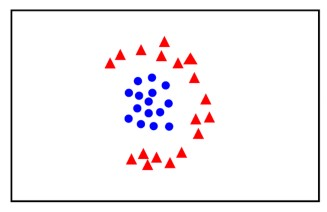
\includegraphics[scale = 1.5]{img/nonlinear svm.jpg}
		\label{svm}
		\caption{Non-linear problem}
\end{figure}

The idea is to define a function $\phi(x)$ that applies a \textbf{mapping} of a \textbf{feature vector} to \textbf{another} one. The SVM algorithm, instead of considering vector $x$, learns using the transformed vector $\phi(x)$. A \textbf{kernel} function is nothing but an \textbf{inner product} between feature mappings of $\phi$:
$$K(x,z) = \phi(x)^T\phi(z)$$

\begin{exmp}
The following Picture represents an example of possible mapping of the data points into a new space in order to make them linearly separable.
    \begin{figure}[h!]
		\centering
		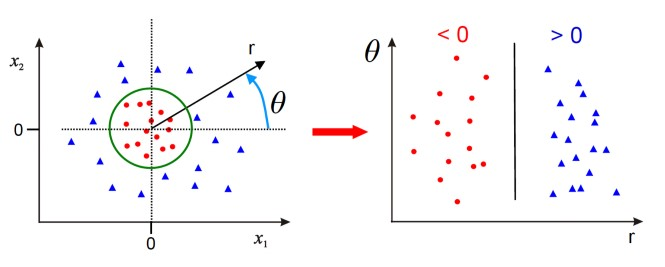
\includegraphics[scale = 1.5]{img/example of transformation.jpg}
		\label{svm}
		\caption{Example of mapping}
\end{figure}

As we can see, data is now represented in polar coordinates (each point is defined by the radius $r$ and the angle $\theta$), so the points are now linearly separable. In this case $\phi : (x_1, x_2)  \in \mathbb{R}^2 \to (r,\theta) \in \mathbb{R}^2$, so in this case we did not project the feature in a larger dimensionality vector.

\end{exmp}

\paragraph{Cover's Theorem} \textit{A complex pattern-classification problem cast in a high-dimensional space non-linearly is more likely to be linearly separable than in a low-dimension space.}\\

In other words, this theorem states that if we map the points of a problem which is not linearly separable into a higher dimensional space, then the problem is more likely to be linearly separable. The \textbf{power} of\textbf{ SVM's} resides in the fact that they represent a \textbf{robust} and \textbf{efficient} \textbf{implementation} of Cover's \textbf{theorem}.

In general, nonlinear SVM's operate in two stages:

\begin{enumerate}
    \item Perform a (typically implicit) \textbf{non-linear mapping} $\phi$ of the feature vector $x$ onto a high-dimensional space that is hidden from the inputs or the outputs. This represents the most difficult step;
    \item Construct an \textbf{optimal separating} \textbf{hyperplane} using SVM's in the high-dimensional space.
\end{enumerate}

We recall that in the dual representation of SVM's the inputs appears only in a \textbf{dot-product form}, i.e.

\begin{equation*}
\begin{aligned}
&\text{max }\quad L_D(\lambda_1,\dots,\lambda_N) = \sum_{i = 1}^{N}\lambda_i - \frac{1}{2}\sum_{i = 1}^{N}\sum_{j = 1}^{N}\lambda_i\lambda_jy_iy_jx_i^Tx_j\\
&\text{s.t.} \quad \sum_{i = 1}^{N}\lambda_iy_i= 0 \qquad \forall i = 1,\dots,N\\
&\text{s.t.} \quad 0 \leq \lambda_i \leq C \qquad \forall i = 1,\dots, N
\end{aligned}
\end{equation*}

and the discriminant function obtained from the solution is:
$$f(x) = \sum\limits_{i = 1}^Ny_i\lambda_ix_i^Tx +b$$

Now we can \textbf{replace} the simple \textbf{inner product} with a \textbf{kernel function} in order to learn in a different feature space, which in some cases could be more efficient. There is a restriction on the function $K$: it must satisfy the following \textbf{property} (called Mercer's condition) in order to be considered a \textbf{valid kernel}:
$$K(x,z) = \phi(x)^T\phi(z) \qquad \forall x, z \in S$$

In this sense, suppose we first \textbf{mapped} the data to some other (possibly infinite dimensional) Euclidean space, using a mapping:
$$x \rightarrow \phi(x) \qquad K(x,y) = \phi(x)^T\phi(y)$$

\begin{equation*}
\begin{aligned}
&\text{max }\quad L_D(\lambda_1,\dots,\lambda_N) = \sum_{i = 1}^{N}\lambda_i - \frac{1}{2}\sum_{i = 1}^{N}\sum_{j = 1}^{N}\lambda_i\lambda_jy_iy_jK(x_i,x_j)\\
&\text{s.t.} \quad \sum_{i = 1}^{N}\lambda_iy_i= 0 \qquad \forall i = 1,\dots,N \\
&\text{s.t.} \quad 0 \leq \lambda_i \leq C \qquad \forall i = 1,\dots,N
\end{aligned}
\end{equation*}

Now, the \textbf{discriminant function} is:

$$f(x) = \sum\limits_{i = 1}^Ny_i\lambda_iK(x_i, x) +b$$

Note that now is \textbf{not necessary} to compute $\phi(x)$.

There exist many kernels, for instance:
\begin{itemize}
	\item \textbf{Linear}: $K(x_i,x_j) = x_i^Tx_j$, which performs an identity mapping;
	\item \textbf{Polynomial kernel}: $K(x_i,x_j) = (1 + x_i^Tx_j)^d$, for any $d > 0$;
	\item \textbf{Gaussian kernel} (RBF): 
	$K(x_i, x_j) = \exp\left(-\frac{\|x_i - x_j\|^2}{2\sigma^2}\right)$, for any $\sigma > 0$.
\end{itemize}
\begin{figure}[!h]
	\begin{minipage}[t]{0.5\linewidth}
		\centering
		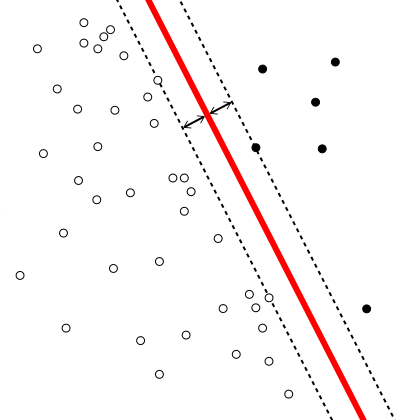
\includegraphics[width=0.41\textwidth]{img/Linear_Kernel_Machine.png}
		\caption{Linear kernel}
		\label{f1}
	\end{minipage}
	\hspace{0.1cm}
	\begin{minipage}[t]{0.5\linewidth} 
		\centering
		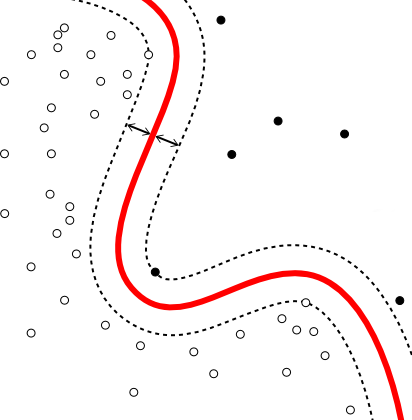
\includegraphics[width=0.41\textwidth]{img/Poly_Kernel_Machine.png}
		\caption{Polynomial kernel}
		\label{f2}
	\end{minipage}        
\end{figure} 
\image{img/RBF_Kernel.png}{Gaussian kernel}{0.3}

\subsection{Multi-class problems}
Thus far we have only discussed about the application of an SVM using \textbf{two labels} $y \in\{-1,1\}$. In real cases, however, we can have more than two classes and we might need to develop an SVM capable of assigning input vectors to one in $K$ \textbf{classes}. In other words, we have to find a decision rule that divides the input space into $K$ \textbf{decision regions} separated by decision boundaries. 
\image{img/multiclass.png}{Decision boundaries for 3 classes.}{0.3}
We can apply two distinct strategies:
\begin{itemize}
	\item \textbf{One-vs-rest classifiers}: train $K-1$ classifiers, \textbf{each} of which solves a \textbf{two-class problem} of separating points in a particular class from points not in that class.
	
	\item \textbf{One-vs-one classifiers}, train $K(K-1)/2$ \textbf{binary classifiers}, one for every possible pair of classes.
	
\end{itemize}

\begin{figure}[!h]
	\begin{minipage}[t]{0.5\linewidth}
		\centering
		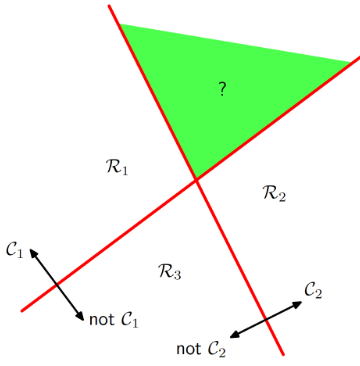
\includegraphics[width=0.51\textwidth]{img/onevsrest.png}
		\caption{One-vs-the-rest classifiers.}
	\end{minipage}
	\hspace{0.1cm}
	\begin{minipage}[t]{0.5\linewidth} 
		\centering
		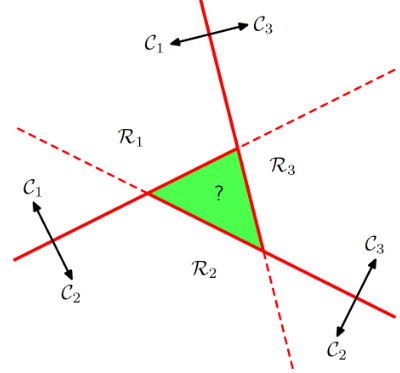
\includegraphics[width=0.51\textwidth]{img/onevsone.png}
		\caption{One-vs-one classifier.}
	\end{minipage}        
\end{figure} 

Note that in the first case the green area denotes a region in which the points are both in $C_1$ and in $C_2$, while in the second case the points in the green area are in $C_1$, $C_2$ and $C_3$ at the same time. Thus, in both cases we have contradictory results. The \textbf{classical approach} consists on training $K$ \textbf{one-vs-rest classifiers} and then the classification is done choosing the \textbf{class} with the ``\textbf{most positive}'' score.

\image{img/learnKclasses.png}{Decision boundaries on typical approaches.}{0.5}

\subsection{Advantages and disadvantages}
Among the \textbf{advantages} we can find:

\begin{itemize}
    \item SVM works relatively \textbf{well} when there is a \textbf{clear margin} of separation between classes;
    \item SVM is\textbf{ more effective} in \textbf{high dimensional spaces} and is relatively memory efficient;
    \item SVM is \textbf{effective} in cases where the \textbf{dimensions are greater than the number of samples}.
\end{itemize}

On the other hand, the \textbf{disadvantages} are:

\begin{itemize}
    \item SVM algorithm is \textbf{not suitable} for \textbf{large data sets};
    \item SVM does \textbf{not perform very well} when the data set has more \textbf{noise} i.e. target classes are overlapping. In cases where the number of features for each data point exceeds the number of training data samples, the SVM will underperform.
    \item As the support vector classifier works by putting data points, above and below the classifying hyperplane there is \textbf{no probabilistic explanation} for the classification.
\end{itemize}
\section{Clustering}

The \textbf{classical clustering} problem starts with 

\begin{itemize}
    \item A set of $n$ objects;
    \item A $n \times n$ matrix $A$ of pairwise similarities that gives us an edge-weighted graph $G$.
\end{itemize}

, and the goal is to \textbf{partition} the vertices of $G$ into \textbf{maximally homogeneous groups (clusters)}. Usually we make the following assumptions:

\begin{itemize}
    \item The \textbf{similarity metric} is \textbf{symmetric}, i.e. $\text{sim}(a,b) = \text{sim}(b,a)$. However, this is not always the case: if, for example, we consider the case of computing a similarity between two documents represented using \textit{bag of words} (each document is represented as a probability distribution of its terms), then the \textit{KL divergence} can be used for computing the similarity, but we've seen that this measure is not symmetric;
    \item We only consider \textbf{pairwise similarities}, i.e. similarity between two objects. Notice that there are situations in which we may compute the similarity between more that 2 objects, e.g. with \textbf{tensors} or \textbf{hypergraphs}.
    \item The graph $G$ is an undirected graph.
\end{itemize}

\image{img/clustering}{The "classical" clustering problem.}{0.8}

Clustering problems abound in many areas of CS, e.g. image processing and CV, IR, document analysis, data mining etc.. If we consider, for example, the image segmentation problem, it's easy to see that it "simply" consists in clustering similar pixels of an image into coherent regions. 

\subsection{Feature-based clustering algorithm: K-means}
K-means is an iterative clustering algorithm that relies on the following assumptions:

\begin{itemize}
    \item It is provided as input with \textbf{feature vectors}, and for this reason we refer to K-means as a \textbf{feature-based} (or \textbf{central}) \textbf{clustering} algorithm, i.e. it receives in input points in a high-dimensional feature space. The other approach is represented by the \textbf{graph-based} (or \textbf{pairwise}) \textbf{clustering} algorithm, in which we are given either a \textbf{similarity matrix} or a \textbf{graph} in which the weights represent the similarity between the entities. In this latter case we do not make any assumption about the representations of the objects;
    \item The \textbf{number of clusters} is known in advance (in many applications this is a problem).
\end{itemize}

The algorithm follows these steps:
\begin{itemize}
	\item \textbf{Initialize:} pick $K$ random points as cluster centers.
	\image{img/kmeans1}{Initialization with $K=2$.}{0.24}
	\item \textbf{Alternate:}
	\begin{enumerate}
		\item \textbf{Assign} data points to \textbf{closest cluster center}.
		\item \textbf{Change the cluster center} to the \textbf{average} of its assigned points.
		\begin{figure}[H]
			\begin{minipage}[t]{0.42\linewidth} 
				\centering
				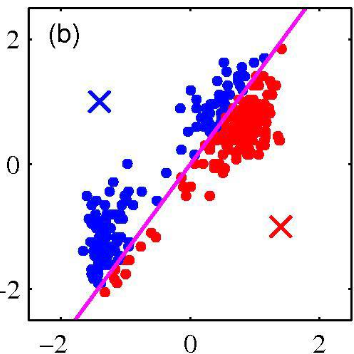
\includegraphics[width=0.58\textwidth]{img/kmeans2}
				\caption{Iterative step 1.}
			\end{minipage}        
			\hspace{2.5cm}
			\begin{minipage}[t]{0.42\linewidth} 
				\centering
				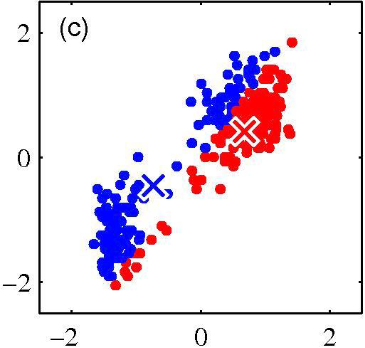
\includegraphics[width=0.58\textwidth]{img/kmeans3}
				\caption{Iterative step 2.}
			\end{minipage}
		\end{figure}
		\FloatBarrier
	\end{enumerate}
	\item \textbf{Stop:} when no points' assignments change.
	\begin{figure}[H]
		\begin{minipage}[t]{0.42\linewidth} 
			\centering
			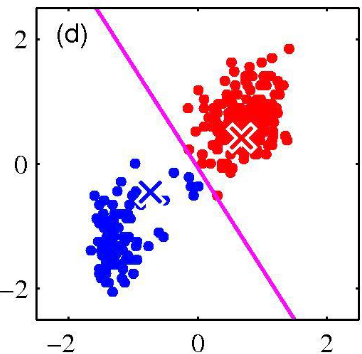
\includegraphics[width=0.58\textwidth]{img/kmeans4}
			\caption{Repeat until convergence.}
		\end{minipage}        
		\hspace{2.5cm}
		\begin{minipage}[t]{0.42\linewidth} 
			\centering
			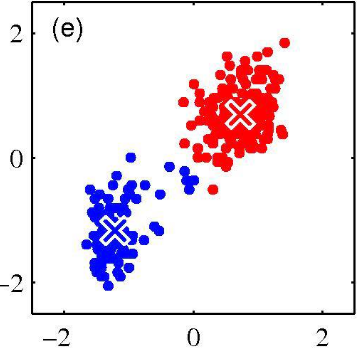
\includegraphics[width=0.58\textwidth]{img/kmeans5}
			\caption{Final output.}
		\end{minipage}
	\end{figure}
\end{itemize}
\paragraph*{Advantages of K-means.} 
\begin{itemize}
        \item It is a \textbf{simple algorithm};
	\item It is guaranteed to \textbf{converge} in a \textbf{finite number of steps};
	\item It \textbf{minimizes} an \textbf{objective function} (i.e. it \textbf{maximizes} the \textbf{compactness} of clusters):
	$$\sum_{i \in \text{clusters}} \Biggl\{ \sum_{j \in \text{elements of i-th cluster}} ||x_j - \mu_i||^2 \Biggr\}$$
	where $\mu_i$ is the center of cluster $i$;
	\item It \textbf{assigns} data points to closest cluster center in $O(Kn)$ and it \textbf{changes} the cluster center to the average of its points in $O(n)$, so it is an \textbf{efficient} algorithm.
\end{itemize}

\paragraph{Disadvantages of K-means}

\begin{itemize}
    \item It converges to a \textbf{local minimum} of the error function, i.e. we have no theoretical guarantees that the algorithm will converge to a global minimum, and that's the reason why we may run the algorithm several times;
    \item It needs to pick $K$ \textbf{initial points}, hence proving to be very \textbf{sensitive to the initialization step};
    \item It is also very sensitive to the \textbf{outliers}, which are not known in advance;
    \item It only finds \textbf{spherical clusters}, due to the objective function it minimizes. In this sense, this algorithm does not work when we have non-convex clusters;
    \item It works with \textbf{feature vectors}, which sometimes are not easy to obtain.
\end{itemize}

\subsection{Eigenvector-based clustering}
As we introduced before, the other possible approach for unsupervised learning is represented by the \textbf{graph-based clustering}, in which the input is represented either by a \textbf{similarity matrix} or a \textbf{graph}.

\begin{figure}[h!]
		\centering
		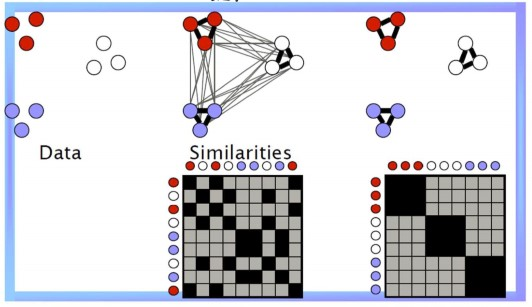
\includegraphics[scale = 1.5]{img/graph matrix clustering.jpg}
		\label{svm}
		\caption{Graph and matrices for clustering}
\end{figure}

It is important to underline the fact that the two representations are equivalent, but they have different characteristics:

\begin{itemize}
    \item If we consider the \textbf{similarity matrix}, then eivenvalues and eigenvectors play a crucial role in the clustering problem, since they provide an information of the matrix which is independent of the permutations of the matrix. In this sense, despite the fact that there may exist many matrices representing the same graph, the resulting eigenpairs remain the same;
    \item If we consider the \textbf{graph} representation, then the notion of \textbf{cut} plays a crucial role in clustering: this problem, indeed, reduces in finding the cut(s) of the graph which separate the object of different classes from the others, i.e. that maximize the \textbf{intra-class similarity} and minimize the \textbf{inter-class similarity}. 
\end{itemize}

We now focus on the clustering problem that deals with a \textbf{similarity matrix}.
\subsubsection{Eigenvalues and eigenvectors}
Before defining the clustering problem as a \textbf{eigenvector-based} problem, we make a little digression on eigenpairs. We first focus on two cases:

\begin{itemize}
    \item Suppose we have a \textbf{symmetric matrix} $A$, then all the \textbf{eigenvalues} are \textbf{real}, which means we can consider an order between the eigenvalues. This property introduces a very strong assumption of the \textbf{spectral graph theory}, i.e. that the input matrix must be symmetric;
    \item Suppose we have a \textbf{non symmetric matrix} $A$, then $A$ must be symmetrized, i.e. we must build a symmetrix matrix $A'$ as:

    $$
    A' = \frac{1}{2} (A + A^T)
    $$
\end{itemize}

Now, suppose that the matrix $A$ is symmetric, we can compute the largest eigenvalue $\lambda_\text{MAX}$ of $A$ by solving one of the following two maximization problem:

\begin{equation}\label{eq_largest lambda1}
\lambda_\text{MAX} = \max_{x} \quad & x^T A x\\
\quad \textrm{ s.t.} \quad & x^T x = 1
\end{equation}

or

\begin{equation}\label{eq_largest lambda2}
\lambda_\text{MAX} = \max_{x} \quad & \frac{x^T A x}{x^T x}\\
\quad \textrm{ s.t.} \quad & x \in \mathbb{R}^n
\end{equation}

, where $\frac{x^T A x}{x^T x}$ is defined as \textbf{Rayleigh quotient}. Notice that \ref{eq_largest lambda1} is a \textbf{constrained optimization problem}, while \ref{eq_largest lambda2} is an \textbf{unconstrained optimization problem}.

On the other hand, the general eigenvector/eigenvalue problem is defined by finding the $\lambda$ s.t. $Ax = \lambda I x$, where $I$ represents the \textbf{identity matrix}: if we have another matrix $B$, then the solution becomes $Ax = \lambda B x$, and the solution of finding $\lambda_\text{MAX}$ is:

\begin{equation}\label{eq_largest lambda3}
\max_{\lambda_\text{MAX}} \quad & \frac{x^T A x}{x^T B x}\\
\quad \textrm{ s.t.} \quad & x \in \mathbb{R}^n
\end{equation}

\subsubsection{Problem definition}
Let us represent a \textbf{cluster} using a \textbf{vector} $x$ whose $i$-th entry captures the participation of node $i$ in that cluster:

$$x_i : \begin{cases}
\neq 0 \text{  if } i \in C\\
= 0 \text{  if } i \notin C
\end{cases}$$

If a node does not participate in a cluster, the corresponding entry is zero. We also impose the \textbf{restriction} that $x^Tx = 1$ in order to avoid the trivial solution $x=0$.\\
Thus, we want to maximize:
$$\sum_{i=1}^n \sum_{j=1}^n w_{ij} x_i x_j = x^TAx$$
which measures the \textbf{cluster's cohesiveness}. In this sense, out goal is to maximize the internal similarity of the points within the cluster. As we introduced in the previous section, this is an \textbf{eigenvalue problem}, which consists in choosing the \textbf{eigenvector} of $A$ corresponding to the \textbf{largest eigenvalue}.\\

From the following image we can see that it could be possible to find clusters by visual inspection of the eigenvectors.

\begin{figure}[H]
	\begin{minipage}[t]{0.49\linewidth} 
		\centering
		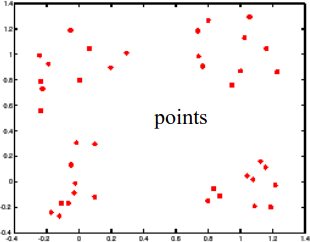
\includegraphics[width=1\textwidth]{img/eigenpoints}
	\end{minipage}        
	\hspace{1cm}
	\begin{minipage}[t]{0.49\linewidth} 
		\centering
		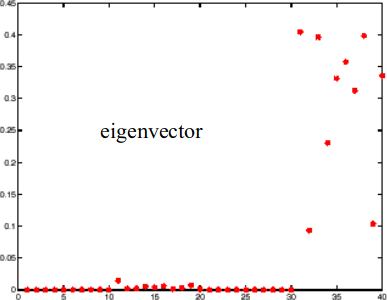
\includegraphics[width=1\textwidth]{img/eigenvectors}
	\end{minipage}
\end{figure}

However, solving the previous problem only allows to find a \textbf{single cluster}, so in case we must extract \textbf{more than two clusters} from the eigenvectors, we can consider one of the following strategies:

\begin{enumerate}
    \item Recursively split each side to get a tree, continuing till the eigenvalues are too small;
    \item Use not only the largest eigenvalue, but also the others. A powerful result in linear algebra says that the second largest eigenvalue (i.e. the eigenvalue associated to the second largest eigenvector) can be obtained by considering 

    \begin{equation}\label{eq_largest lambda3}
    \max \quad & \frac{x^T A x}{x^T x}\\
    \quad \textrm{ s.t.} \quad & x \in \mathbb{R}^n \text{and } x \perp x_\text{max}
    \end{equation}
    , where $x_\text{max}$ represents the eigenvector associated to the largest eigenvalue.
    
\end{enumerate}

\subsubsection{Clustering by eigenvectors : algorithm}
The algorithm that builds the clusters through the eigenvectors performs the following steps:
\begin{enumerate}
	\item Construct (or take as input) the \textbf{affinity matrix} $A$;
	\item Compute the \textbf{eigenvalues} and \textbf{eigenvectors} of $A$;
	\item Repeat until there are sufficient clusters:
	\item $\quad$ Take the \textbf{eigenvector} corresponding to the \textbf{largest} unprocessed \textbf{eigenvalue};
	\item $\quad$ \textbf{Zero} all the components corresponding to \textbf{elements} that have already \textbf{been clustered};
	\item $\quad$ \textbf{Threshold} the remaining components to determine which elements belong to this cluster;
	\item $\quad$ If all elements have been accounted for, there are sufficient clusters;
\end{enumerate}

\subsection{Graph-based clustering algorithm}
If we consider the \textbf{graph} representation we have that:
\begin{itemize}
	\item A \textbf{node} represents each of the \textbf{pixels};
	\item An \textbf{edge} between every pair of pixels (or every pair of "sufficiently close" pixels), which is weighted according to the affinity or \textbf{similarity} of the two nodes.
\end{itemize}  
\image{img/imageasgraph}{Image as a graph.}{0.7}
If we suppose to represent each \textbf{pixel} with a \textbf{feature vector} $x$ and to define a \textbf{distance function} appropriate for this feature representation, then we can \textbf{convert} the \textbf{distance} between two feature vectors into an \textbf{affinity} with the help of a \textbf{Gaussian kernel}:
$$exp\left(-\frac{1}{2\sigma^2} dist(x_i, x_j)^2\right)$$
Notice that we can exploit this kernel to transform a feature-based dataset into a graph-based one. We can notice that the \textbf{similarity} of two data points is \textbf{inversely proportional} to their \textbf{distance}, and we also underline the importance of the \textbf{scale} parameter $\sigma$: the \textbf{smaller} $\sigma$, the \textbf{more rigid} will be the clustering algorithm in grouping together only nearby points; on the other hand, the \textbf{larger} $\sigma$, the more the algorithm will \textbf{group} together \textbf{far-away points}.

We now focus on the clustering as a \textbf{graph partitioning problem}. Let $G=(V,E,w)$ be an undirected weighted graph, i.e. the similarity matrix is symmetric, and given a partition (or cut) $(C_1, C_2)$ of the graph $G$, then the following quantity can be defined:

$$
cut(C_1,C_2) = \sum_{i \in C_1} \sum_{j \in C_2} w(i,j)
$$

In Picture \ref{cut}, the cut of the two sub graphs is given by the sum of the weights of the red edges.

\begin{figure}[h!]
		\centering
		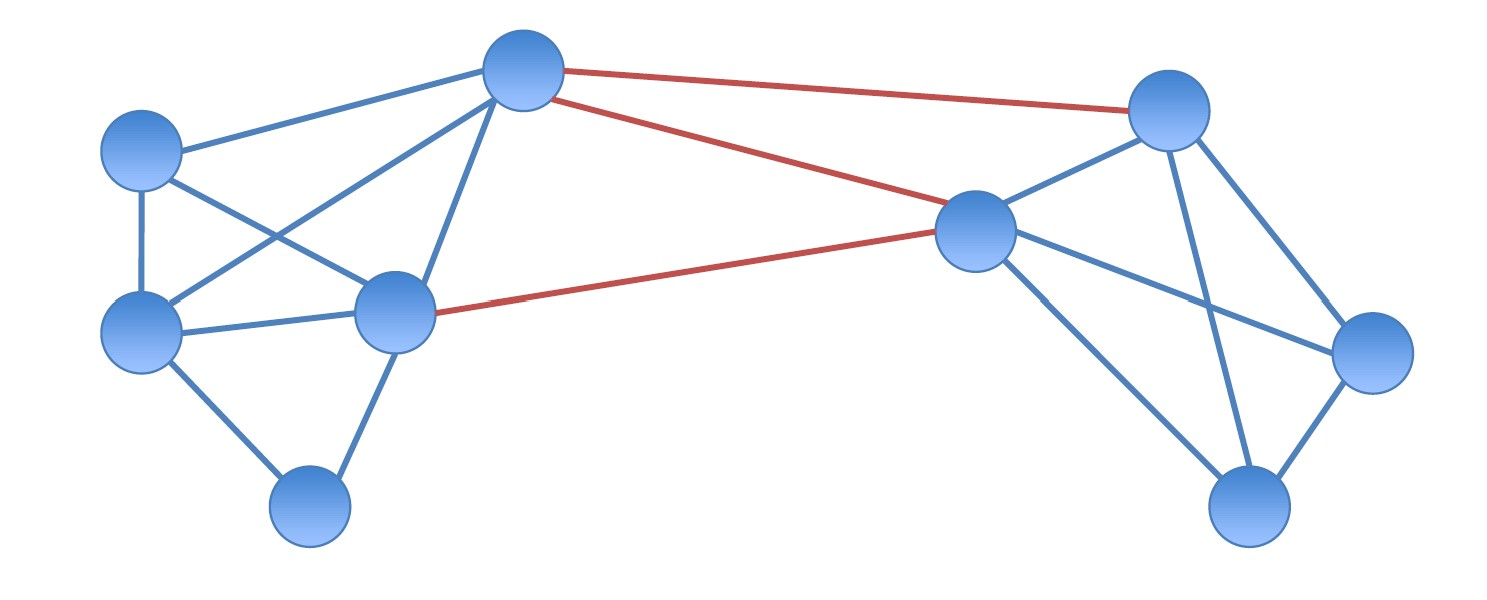
\includegraphics[scale = 0.6]{img/cut.jpg}
		\label{cut}
		\caption{Cut in a graph}
\end{figure}

\paragraph{Minimum cut}
\\
Given this quantity, we can easily connect the problem of determine the clusters of a graph to the one of finding a cut that maximizes the intra-cluster similarity and minimizes the inter-class similarity of the points contained in the two partitions that are formed. More specifically, finding the clusters in a graph is equal to solve the so called \textbf{minimum cut problem}. This problem tries to find the cut that minimizes the quantity $cut(C_1, C_2)$ among all the possible cuts, i.e. partitions, $(C_1, C_2)$.

Despite the fact that the number of cuts in a graph grows exponentially with the number of nodes, an important property of the \textit{minimum cut} problem is that it is solvable in polynomial time. However, a quite important disadvantage of this problem is that it favors highly unbalanced clusters, in particular the ones composed by single vertices, as represented in Picture \ref{problem}.

\begin{figure}[h!]
		\centering
		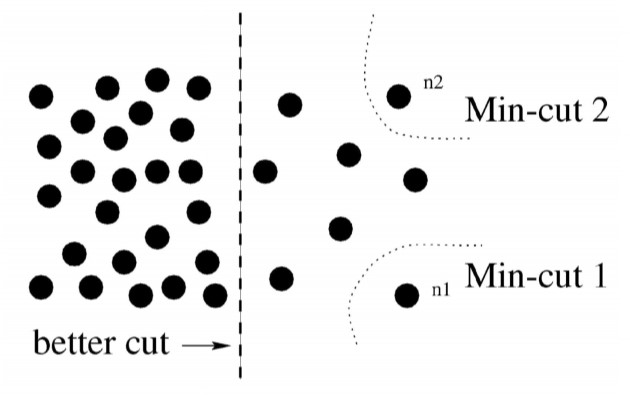
\includegraphics[scale = 1.0]{img/min cut problem.jpg}
		\label{problem}
		\caption{Disadvantage of MinCut problem: isolated vertices form a cluster}
\end{figure}

This problem derives from the fact that it takes into account only the intra-cluster similarity, resulting in this kind of undesired partitions.

\paragraph{Normalized cut}
\\
The other possible approach when dealing with graph partitioning, and the one adopted in this project, is represented by solving the \textbf{normalized cut} problem. Before discussing the details of this problem, we introduce some important metrics:

\begin{itemize}
    \item the \textit{degree} of a node is defined as $\text{deg}(i) = \sum_j w_{i,j}$, i.e. it is represented by the sum of the values in the i-th row of the matrix representing the graph;
    \item the \textit{volume} of a set of nodes is defined as $vol(A) = \sum_{i \in A} d_i$, where $A \subseteq V$, i.e. it is represented by the sum of the degrees of the nodes in the set (sum of multiple rows).
\end{itemize}

The idea of \textit{normalized cut} is to overcome the limits of \textit{minimum cut} by normalizing the previous quantity by a measure (the volume) that allows to combine both the intra-cluster similarity and the inter-cluster similarity. More specifically, for the \textit{normalized cut} problem, the quantity that has to be minimized is the following one:

$$
Ncut(C_1,C_2) = cut(C_1, C_2) \left( \frac{1}{vol(C_1)} + \frac{1}{vol(C_2)} \right)
$$

Despite providing more accurate clusters, the crucial issue about \textit{normalized cut} is that finding its minimum is \textbf{NP-hard}, and for this reason there exist some efficient approximations that exploit the properties of linear algebra. One of this approximations is based on the \textbf{graph Laplacian} or \textbf{Laplacian matrix}, which is a matrix defined as:

$$
L = D - W
$$

, where:

\begin{itemize}
    \item $D$ is the \textit{diagonal degree matrix}, i.e. $d_{ii} = \text{deg}(i) = \sum_j w_{i,j}$;
    \item $W$ is the \textit{similarity matrix}, in which the elements of the diagonal are equal to 0 by definition. Moreover, if the graph is unweighted, then $W$ only contains 1s and 0s. 
\end{itemize}

In this sense, the elements of $L$ are given by:

$$
L _ { i , j } = \left\{ \begin{array} { l l } { \operatorname { d } \left( v _ { i } \right) } & { \text { if } i = j } \\ 
{ - 1 } & { \text { if } i \neq j \text { and } v _ { i } \text { is adjacent to } v _ { j } } \\ 
{ 0 } & { \text { otherwise } } \end{array} \right.
$$

This is an example of the degree matrix $D$ and the affinity matrix $W$ in relation to the graph of the next page.
\begin{figure}[H]
	\begin{minipage}[t]{0.49\linewidth} 
		\centering
		$$ D = \begin{bmatrix}
		2 & 0 & 0 & 0 & 0 & 0 \\
		0 & 4 & 0 & 0 & 0 & 0 \\
		0 & 0 & 4 & 0 & 0 & 0 \\
		0 & 0 & 0 & 1 & 0 & 0 \\
		0 & 0 & 0 & 0 & 3 & 0 \\
		0 & 0 & 0 & 0 & 0 & 2 \\
		\end{bmatrix}$$
		\caption{Degree matrix $D$.}
	\end{minipage}        
	\hspace{1cm}
	\begin{minipage}[t]{0.49\linewidth} 
		\centering
		$$ W = \begin{bmatrix}
		0 & 1 & 1 & 0 & 0 & 0 \\
		1 & 0 & 1 & 1 & 1 & 0 \\
		1 & 1 & 0 & 0 & 1 & 1 \\
		0 & 1 & 0 & 0 & 0 & 0 \\
		0 & 1 & 1 & 0 & 0 & 1 \\
		0 & 0 & 1 & 0 & 1 & 0 \\
		\end{bmatrix}$$
		\caption{Affinity matrix $W$.}
	\end{minipage}
\end{figure}

\image{img/graphLaplacian}{Example of laplacian graph.}{0.85}

The \textit{Laplacian matrix} $L$ satisfies the following \textbf{properties}:
\begin{enumerate}
        \item $L \in \mathbb{R}^{n \times n}$ and the sum of rows/columns is always 0;
	\item For all vectors $x$ in $\mathbb{R}^n$, we have:
	$$x ^ T L x = \frac { 1 } { 2 } \sum _ { i, j = 1 } ^ { n } w _ { i j } \left( x _ { i } - x _ { j } \right) ^ { 2 } \geq 0$$
	This is proved as follows:
	$$\begin{aligned} 
	x ^ { T } L x & = x^T (D-W) x = x ^ { T } D x - x ^ { T } W x = \sum _ { i=1 }^n d _ { i } x _ { i } ^ { 2 } - \sum _ { i , j =1 }^n x _ { i } x _ { j } w _ { i j } \\ 
	& = \frac{1}{2} \left( \sum_i \sum_j d_{ij} x_i x_j - 2 \sum_i \sum_j w_{ij} x_i x_j + \sum_i \sum_j d_{ij} x_i x_j \right) \\ 
        & = \frac{1}{2} \left( \sum_i d_{ii} x_i^2 - 2 \sum_i \sum_j w_{ij} x_i x_j + \sum_j d_{jj} x_j^2 \right) \\
        & = \frac{1}{2} \left( \sum_i (\sum_j) w_{ij} \right) x_i^2 - 2 \sum_i \sum_j w_{ij} x_i x_j + \sum_j (\sum_i w_{ji}) x_j^2 \\
        & = \frac{1}{2} \left( \sum_i \sum_j w_{ij}x_i^2 - 2 \sum_i \sum_j w_{ij}x_i x_j + \sum_i \sum_j w_{ij} x_j^2 \right) \\
        & = \frac{1}{2} \left( \sum_i \sum_j w_{ij} (x_i^2 - 2 x_i x_j + x_j^2) \right) \\
        & = \frac{1}{2} \left( \sum_i \sum_j w_{ij} (x_i - x_j)^2 \right)

	\end{aligned}$$

        However, since both $w_{ij}$ and $(x_i - x_j)^2$ are $\geq 0$, then $x^TLx \geq 0$.
	 
	\item $L$ is a \textbf{symmetric} and \textbf{positive semi-definite} matrix. The symmetry of $L$ follows directly from the symmetry of $W$ and $D$, while the positive semi-definiteness is a direct consequence of the first property, which shows that $x ^ { T } L x \geq 0$. Notice that the positive semi-definiteness implies that all the eigenvalues are non negative, which has crucial consequences in optimization;
	 
	\item The smallest eigenvalue of $L$ is 0 and the corresponding eigenvector is the constant 1 vector. Moreover, $L$ has $n$ non-negative, real-valued eigenvalues $0 = \lambda _ { 1 } \leq \lambda _ { 2 } \leq \ldots \leq \lambda _ { n }$.
 
\end{enumerate}

More specifically, an important consequence of these properties is that the \textbf{multiplicity}, i.e. the number of eigenvectors associated to a specific eigenvalue, of the smallest eigenvalue $\lambda_1=0$ is the \textbf{number of connected components} $A_1, \dots, A_k$ of the graph. 

\paragraph{The normalized graph Laplacians} There are two matrices which are called normalized graph Laplacians in the literature. Both matrices are closely related to each other and are defined as:
$$\begin{array} { l } { L _ { \mathrm { sym } } = D ^ { - 1 / 2 } L D ^ { - 1 / 2 } = I - D ^ { - 1 / 2 } W D ^ { - 1 / 2 } } \\ { L _ { \mathrm { rw } } = D ^ { - 1 } L = I - D ^ { - 1 } W } \end{array}$$
We denote the first matrix by $L_{sym}$ as it is a symmetric matrix, and the second one by $L_{rw}$ as it is closely connected to a random walk.

\subsubsection{Solving normalized cut}
Any cut $(A,B)$ can be represented by a binary indicator vector $x$:

$$
x_i = \begin{cases}
+1 \text{  if } i \in A\\
-1 \text{  if } i \in B
\end{cases}
$$

, and it can be shown that:

$$
\min_x ~ \text{Ncut}(x) = \min_y \underbrace{\frac{y^T(D-W)y}{y^TDy}}_{\text{Rayleigh quotient}}
$$

subject to the constraint that $y ^ { \prime } D = \sum_{i} y_{i} d _ { i } = 0$, with $y _ { i } \in \{ 1 , - b \}$. Indeed, $y$ is an indicator vector with 1 in the $i$-th position if the $i$-th feature point belongs to $A$, negative constant ($-b$) otherwise ). Again, this problem is still \textbf{NP-hard}, so if we \textbf{relax} the constraint of $y$ to be a discrete-valued vector and allow it to take on real values, the original problem
$$
\min _ { y } \frac { y ^ T ( D - W ) y } { y ^ T D y }
$$

will be equivalent to:
$$
\min _ { y }  y ^ T ( D - W ) y \quad \text { s.t. } \quad y ^ T D y = 1
$$

This amounts to solve a \textit{generalized} eigenvalue problem:
$$
\underbrace{(D-W)}_{Laplacian}y=\lambda D y
$$

\paragraph{2-ways Ncut} Finally, we can provide a \textbf{solution} of the \textit{normalized cut} problem by exploiting this \textbf{algorithm}:

\begin{enumerate}
	\item Represent the \textbf{data points} as a \textbf{weighted graph} $G = (V,E)$, compute the weights of each edge and summarize them into $D$ and $W$;
	\item Solve the generalized eigenvalue problem $(D-W)y = \lambda Dy$ for the \textbf{eigenvector} associated the \textbf{second smallest eigenvalue} (we choose the second smallest eigenvalue since the eigenvector associated to the smallest eigenvalue is equal to 1, while the smallest eigenvalue is equal to 0, and it corresponds to the trivial partition $A = V$ and $B = \{\}$);
	\item Use the entries of the eigenvector to create a partition of the graph into two parts.
\end{enumerate}

Sometimes there's not a \textbf{clear threshold} to split based on the second vector since it takes continuous values. In which way it is possible to choose the splitting point?
\begin{itemize}
	\item Pick a constant value (0 or 0.5).
	\item Pick the median value as splitting point.
	\item Look for the splitting point that has minimum Ncut value:
	\begin{enumerate}
		\item Choose $n$ possible splitting points.
		\item Compute Ncut value.
		\item Pick minimum.
	\end{enumerate}
\end{itemize}

\subsubsection{Relaxation}
As we can see, in order to formalize the \textit{minimum cut problem} we had to \textbf{relax} the constraint owf $y$: the goal of relaxation is then to \textbf{relax the constraints} of a difficult problem and to solve the simpler problem. If we're lucky, the solution we obtain satisfies the original constraints, so we found a solution of the original problem, otherwise we can choose the nearest point that satisfies the original constraints.

Through relaxation we lose some precision in the final solution. Note that the \textbf{original} normalized cut problem returns \textbf{binary values} $(-1,1)$, indicating clustering membership. The \textbf{relaxed version}, on the right, returns \textbf{continuous values}. It may happen that \textbf{some points do not clearly belong to a specific cluster}, as they are close to the margin between the two clusters. For this reason the relaxed solution is \textbf{not} always in a \textbf{one-to-one correspondence} with the original problem, and choosing a ``\textbf{correct}'' threshold is very important.
\imageb{img/relaxation1}{0.8}

\subsubsection{Normalized cut with more than 2 clusters}
There are two possible approaches if we desire to obtain more than 2 clusters:
\paragraph*{Approach \#1.} It recursively performs the 2-way Ncut algorithm until we obtain the desired number of clusters (not so common).
\begin{enumerate}
	\item Given a weighted graph $G=(V,E,w)$, summarize the information into matrices $W$ and $D$.
	\item Solve $(D-W)y = \lambda Dy$ for eigenvectors with the smallest eigenvalues.
	\item Use the eigenvector with the second smallest eigenvalue to bipartition the graph by finding the splitting point such that Ncut is minimized.
	\item Decide if the current partition should be subdivided by checking the stability of the cut, and make sure Ncut is below the prespecified value.
	\item Recursively repartition the segmented parts if necessary.
\end{enumerate}
\textbf{Note:} this approach is \textbf{computationally wasteful}, only the second eigenvector is used, whereas the next few small eigenvectors also contain useful partitioning information.

\paragraph*{Approach \#2.} Using the first $k$ eigenvectors (far more popular).
\begin{enumerate}
	\item Construct a similarity graph and compute the unnormalized graph Laplacian $L$.
	\item Compute the $k$ smallest \textbf{generalized} eigenvectors $u _ { 1 } , u _ { 2 } , \dots , u _ { k }$ of the generalized eigenproblem $L u = \lambda D u$.
	\item Let $U = \left[ u_1, u_{ 2 }, \dots, u_{ k } \right] \in \mathbb { R } ^ { n \times k }$, i.e. the columns are the $k$ eigenvectors we computed.
	\item Let $y_i \in \mathbb{ R }^k$ be the vector corresponding to the $i$th row of $U$.
	$$U = \left[ \begin{array} { c c c c } { u _ { 11 } } & { u _ { 12 } } & { \cdots } & { u _ { 1 k } } \\ { u _ { 21 } } & { u _ { 22 } } & { \cdots } & { u _ { 2 k } } \\ { \vdots } & { \vdots } & { \ddots } & { \vdots } \\ { u _ { n 1 } } & { u _ { n 2 } } & { \cdots } & { u _ { n k } } \end{array} \right] = \left[ \begin{array} { c } { y _ { 1 } ^ { T } } \\ { y _ { 2 } ^ { T } } \\ { \vdots } \\ { y _ { n } ^ { T } } \end{array} \right]$$
	\item Thinking of $y_i$'s as points in $\mathbb{ R }^k$, cluster them with $k$-means algorithms. Why do we use k-means? The rows of $U$ allow to map the vertices of the graph in a 2-dimensional vector (like a projection), and it was proved that this mapping facilitates the use of the k-means algorithm.
\end{enumerate}

\textbf{Note:} the number $k$ of clusters must be known in advance.

\subsubsection{Spectral clustering vs $k$-means}
First of all, let us define the intuition behind \textbf{spectral clustering}: its goal is to cluster data that is connected but not necessarily compact or clustered within convex boundaries. This algorithm is very similar to the previous one, but it has 2 main differences; it works as follows
\begin{enumerate}
	\item Construct a similarity graph and compute the normalized graph Laplacian $L_{sym}$.
	\item Embed data points in a low-dimensional space (spectral embedding), in which the clusters are more obvious, computing the $k$ smallest eigenvectors $v_1, \dots, v_k$ of $L_{sym}$. 
	\item Let $V=\left[v_1,\dots, v_k \right] \in \mathbb{ R }^{n \times k}$.
	\item Form the matrix $U \in \mathbb{ R }^{n \times k}$ from $V$ by normalizing the row sums to have norm 1, that is: 
	$$u_ { i j } = \frac { v _ { i j } } { \left( \sum _ { k } v _ { i k } ^ { 2 } \right) ^ { 1 / 2 } }$$
	\item For $i=1,\dots, n$, let $y _ { i } \in \mathbb { R } ^ { k }$ be the vector corresponding to the $i$th row of $U$.
	\item Cluster the points $y_i$ with $i=1,\dots,n$ with the $k$-means algorithm into clusters $C_1, \dots, C_k$.
\end{enumerate}
The differences with the previous algorithm are following:

\begin{itemize}
    \item We compute a \textbf{normalized graph Laplacian} $L_{\text{sym}}$;
    \item The rows of $U$ are normalized to norm 1.
\end{itemize}

Applying $k$-means to Laplacian eigenvectors allows us to find \textbf{cluster} with \textbf{non-convex boundaries}.

\imageb{img/spectral1}{0.65}
\imageb{img/spectral2}{0.65}
\imageb{img/spectral3}{0.65}

As we said before, one of the main \textbf{issue} of k-means is represented by the choice of the value of $k$: one of the possible solutions (called \textbf{eigengap heuristic}) is to choose $k$ such that all eigenvalues $\lambda_1, \dots, \lambda_k$ are very small, but $\lambda_{k+1}$ is relatively large. In this way, the choosing of $k$ maximizes the eigengap (difference between consecutive eigenvalues) $\delta_k = |\lambda_k - \lambda_{k-1}|$.
\imageb{img/eigengap}{0.75}

\section{Dominant-set clustering}
A very important limitation of the clustering algorithms we've seen so far (especially the \textbf{partition-based} one) is that they're not able to separate the structure of the data from the clutter: this happens because they're goal is to locate distinct coherent clusters, but they do not work very well in presence of noise.

\imageb{img/dominant_init}{0.55}

Indeed, in certain real-world problems, natural groupings are found among only on a small subset of the data, while the rest of the data shows little or no clustering tendencies. In such situations, it is often \textbf{more important} to \textbf{cluster a small subset} of the data very well, \textbf{rather} than \textbf{optimizing} a \textbf{clustering criterion} over \textbf{all the data points}, particularly in application scenarios where a large amount of noisy data is encountered.

Moreover, while partitional approaches impose that each element cannot belong to more than one cluster, this new approach allows to also consider nodes belonging to two different clusters, hence considering the hypothesis of \textbf{overlapping clusters}.

\imageb{img/dominant_overlapping}{0.7}

\subsection{Graph-theoretic definition of a cluster}
Data to be clustered are represented as an undirected weighted graph with no self-loops: $G=(V, E, \omega)$, where $V=\{1,\dots,n\}$ is the vertex set, $E\subseteq V\times V$ is the edges set and $w: E\rightarrow \mathbb{R}^*_+$ is the positive weight function. Vertices represent data points, edges neighborhood relationships and edge-weights similarity relations. $G$ is then represented with an adjacency matrix $A$, such that $a_{ij} = \omega(i,j)$. Since there are not self-loops we have that $\omega(i,i) = 0$ (main diagonal equal to $0$). From now on, if not otherwise stated, $A$ will represent such matrix. \\
There is \textbf{not} an \textbf{unique} and well defined \textbf{definition} of \textbf{cluster}, but the available literature agrees in two conditions that a cluster should satisfy:
\begin{itemize}
  \item \textbf{High internal homogeneity}, also named \textit{internal criterion}. It means that all the objects inside a cluster should be highly similar to (or have low distance from) each other;
  \item \textbf{High external inhomogeneity}, also named \textit{external criterion}. It means that objects coming from different clusters have low similarity (or high distance).
\end{itemize}
The idea of these criterion is that \textbf{clusters} are groups of objects which are \textbf{strongly similar} to each other if they belong to the same cluster, otherwise they are \textbf{highly dissimilar}. 

\paragraph{Basic definitions.}

Let $S\subseteq V$ be a nonempty subset of vertices and $i \in S$. The \textbf{average weighted degree} of $i$ w.r.t. $S$ is defined as:
\begin{equation}
  \text{awdeg}_S(i)=\frac{1}{|S|}\sum_{j\in S}a_{ij}
\end{equation}
, i.e. it represents the \textbf{average similarity} between entity $i$ and the rest of the entities in $S$. It can be observed that $\text{awdeg}_{\{i\}}(i) = 0$  $\forall i \in V$, since we have no self-loops.\\

\image{img/awdeg.png}{Average weighted degree.}{0.25}

We now introduce a new quantity $\phi$ such that if $j \notin S$:
\begin{equation}
  \phi_S(i, j)=a_{ij}-\text{awdeg}_S(i)
\end{equation}

Intuitively, $\phi_S(i, j)$ measures the \textbf{relative similarity} between $i$ and $j$ with respect to the \textbf{average similarity} between $i$ and its neighbors in $S$. This measures can be either positive or negative.

Let $S\subseteq V$ be a nonempty subset of vertices and $i \in S$. The \textbf{weight} of $i$ w.r.t. $S$ is:
\begin{equation}
  w_S(i)= \begin{cases}
      1 & \text{if } |S| = 1 \text{  (singleton)}\\
      \sum\limits_{j\in S\setminus \{i\}}\phi_{S\setminus \{i\}}(j, i)w_{S\setminus \{i\}}(j) & \text{otherwise}
  \end{cases}
\end{equation}

Furthermore, the \textbf{total weight} of $S$ is defined to be $W(S)=\sum_{i\in S}w_S(i)$.
\image{img/ws.png}{Weight of i w.r.t. the elements in S.}{0.18}
Note that $w_{\{i, j\}}(i)=w_{\{i, j\}}(j)=a_{ij}$ $\forall i, j \in V \land i\neq j$. Then, $w_S(i)$ is computed simply as a function of the weights on the edges of the sub-graph induced by $S$.

Intuitively, $w_S(i)$ gives a measure of the \textbf{similarity} between $i$ and $S\setminus \{i\}$ with respect to the \textbf{overall similarity} among the vertices of $S\setminus \{i\}$. In other words, it represents \textbf{how similar (important)} $i$ is \textbf{with respect to the entities} in $S$. An important property of this definition is that it induces a sort of \textbf{natural ranking} among the \textbf{vertices} of the graph. 

\begin{figure}[h!]
		\centering
        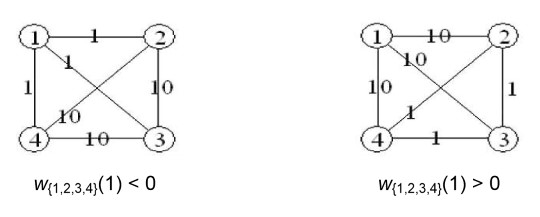
\includegraphics[scale = 1.0]{img/total weight rxample.jpg}
		\label{mi}
        \caption{Examples of total weight}
\end{figure}

As we can see, in the first example we should not add node 1 to the cluster \{1,2,3\}, since it has a low similarity compared with the other nodes (as it can be seen from the value of the total weight), while in the second case we would add node 1 in order to obtain a larger and more coherent cluster.

\paragraph{Dominant set.} A nonempty subset of vertices $S\subset V$ such that $W(T)>0$ for any nonempty $T \subseteq S$, is said to be a \textbf{dominant set} if:
\begin{itemize}
  \item $w_S(i) > 0$, $\forall i \in S \qquad$ (\textit{internal homogeneity})
  \item $w_{S \cup \{i\}}(i) < 0$, $\forall i \notin S \qquad$ (\textit{external homogeneity})
\end{itemize}
These conditions correspond to cluster properties (\textbf{internal homogeneity} and \textbf{external in-homogeneity}). Informally we can say that the \textbf{first condition} requires that \textbf{all the nodes} in the clusters are \textbf{important} for it. The \textbf{second} one assumes that if we consider a \textbf{new point} in the cluster, the \textbf{cluster cohesiveness will be lower}, meaning that the current cluster should be already maximal.\\
By definition, dominant sets are expected to capture \textbf{compact structure}s. Moreover, this definition is equivalent to the one of maximal clique problem when applied to unweighted graphs.

\image{img/dominant_def}{The set of vertices \{1,2,3\} is dominant.}{0.2}

\subsection{Connections of dominant sets}
Dominant sets have intriguing connections with:

\begin{itemize}
    \item \textbf{Game theory}, and concepts like Nash equilibria;
    \item \textbf{Optimization theory}, in particular they are local maximizers of (continuous) quadratic problems;
    \item \textbf{Graph theory} and \textbf{maximal cliques};
    \item \textbf{Dynamical systems theory}.
\end{itemize}

\subsubsection{Game theory}
Game theory is the study of \textbf{mathematical models} of strategic interaction between rational decision-makers. In this sense we can model a new \textbf{clustering game} with the following properties:
\begin{itemize}
	\item \textbf{Symmetric game}, the payoffs for playing a particular strategy depend only on the other strategies employed, not on who is playing them;
	\item \textbf{Complete knowledge}, payoffs, strategies and types of players are known;
	\item Pre-existing set of \textbf{pure strategies}. Players do not behave “rationally” but act according to a pre-programmed behavioral pattern (pure strategy).
\end{itemize}
Data points $V$ are the pure strategies available to the players and the similarity matrix $A$ represents the \textbf{payoff matrix}, which resumes the revenues that each player obtains when a pair of strategies is played. The values $A_{ij}$ and $A_{ji}$ are the revenues obtained by player 1 and player 2 considering that they have player strategies $(i,j) \in V\times V$.
A \textbf{mixed strategy} $x=(x_1, \dots, x_n)^T \in \Delta$ is a probability distribution over the set of pure strategies, which models a stochastic playing strategy of a player. If player 1 and 2 play mixed strategies $(x_1, x_2) \in \Delta \times \Delta$, then the expected payoffs for the players are: $\mathbf{x_1^TAx_2}$ and $\mathbf{x_2^TAx_1}$ respectively.
The goal of the two players of course is to maximize their resulting revenue as much as possible. During the game each player extracts an object $(i,j)$ and the resulting revenue is associated
according to the payoff matrix $A$. Since we are considering $A$ as equal to the similarity matrix, we can say that in order to \textbf{maximize} their revenues the two players should \textbf{coordinate} their strategies so that the \textbf{extracted objects belong to the same cluster}. In other words, only by selecting objects belonging to the same cluster, each player is able to maximize his expected payoff. The unique difference is that the similarity between two equal entities is $0$, meaning that $A_{ii} = 0$. The desired condition is that the two players reach a \textbf{symmetric Nash equilibrium}, a state in which the two players agree about the cluster membership. A \textbf{Nash equilibrium} is a mixed-strategy profile $(x_1,x_2)\in \Delta\times \Delta$ such that no player can improve the expected payoff by changing his playing strategy, given the opponent's strategy being fixed. In other words, it is a \textbf{configuration of strategies} for which \textbf{no player} will deviate from it for its convenience since there is \textbf{no incentive} to change choice. This concept can be expressed with the following expression:
$$y_1^TAx_2 \leq x_1^TAx_2 \qquad y_2^TAx_1 \leq x_2^TAx_1 \qquad \forall (y_1,y_2) \in (V\times V).$$ 
A Nash equilibrium is \textbf{symmetric} if $x_1 = x_2$, meaning that considering a symmetric Nash equilibrium $x \in \Delta$ the two conditions hold in a unique one:
$$y^TAx \leq x^TAx$$

This condition satisfies the \textbf{internal homogeneity} criterion required by the dominant set definition, but it does \textbf{not} include any kind of constraint that guarantees the \textbf{maximality condition}. In order to satisfy this condition it is necessary to look for a different type of Nash Equilibrium, known as \textbf{Evolutionary Stable Strategy (ESS)}. 

\paragraph{ESS.} A symmetric Nash equilibrium $x\in \Delta$ is an \textbf{evolutionary stable strategy} (ESS) if it satisfies also:
$$y^TAx = x^TAx \implies x^TAy > y^TAy \qquad \forall y \in \Delta\setminus\{x\}$$

$$y^TAx = x^TAx \implies x^TAy < x^TAx \qquad \forall y \in \Delta\setminus\{x\}$$
Even if the strategy $y$ provides the same payoff of the strategy $x$, it is better to play $x$ since the payoff against itself is greater than the one provided by $y$. The two strategies $x$ and $y$ represents two Nash Equilibrium, but only $x$ is an ESS.\\
In conclusion we can say that the \textbf{ESSs of the clustering game} with affinity matrix $A$ are in \textbf{correspondence} with \textbf{dominant sets} of the same clustering problem instance. However, we can also conclude that \textbf{ESSs} are in \textbf{one-to-one} correspondence to \textbf{(strict) local solutions of StQPs} (Standard Quadratic optimization Problems).\\
It is possible to say that ESSs abstract well the main characteristic of a cluster:
\begin{itemize}
	\item \textbf{Internal coherency:} High mutual support of all elements within the group.
	\item \textbf{External incoherency:} Low support from elements of the group to elements outside the group.
\end{itemize}

\subsubsection{Optimization theory}
\textbf{Clusters} are commonly represented as $n$-dimensional \textbf{vectors} expressing the participation of each node to a cluster. Large numbers denote a strong participation, while zero values no participation. The \textbf{cohesiveness} of a cluster can be computed using:
\begin{equation}
f(x)=x^\top Ax
\end{equation}
where $A$ is the \textbf{symmetric} real-valued matrix with null diagonal. \textbf{Clustering} can now be formulated as the problem of \textbf{finding the vector} $x$ that \textbf{maximizes} $f$. The objective function has to be \textbf{normalized}. For this aim simplex constraints are imposed. This yields the following \textbf{standard quadratic optimization problem} whose \textbf{local solution} corresponds to a \textbf{maximally cohesive cluster}:
\begin{equation}\label{SPQ}
\begin{array}{lcl}
\text{max} & x^TAx \\
\text{s.t.} & x \in \Delta
\end{array}
\end{equation}
where
\begin{equation}
\Delta=\{x\in\mathbb{R}^n:x\geq 0 \land x^\top x = 1\}
\end{equation}
is the \textbf{standard simplex} of $\mathbb{R}^n$.\\

\image{img/standardSimplex.png}{Standard simplex on $\mathbb{R}^3$.}{0.35}

As we can see, this problem is quite similar to the one presented in the previous Chapter, but the difference relies in the constraint.

In conclusion \textbf{dominant sets} can be put in \textbf{one-to-one correspondence} (modulo a technical condition) with \textbf{strict local maximizers} of a \textbf{quadratic function over the simplex}. As opposed to many other clustering algorithms, which try to find the global optimum of some energy function, dominant sets can be found by mining local solutions.

\subsubsection{Graph theory and maximal cliques}
Suppose we have a \textbf{binary similarity matrix} and an unweighted undirected graph $G = (V,E)$, then:

\begin{itemize}
    \item A \textbf{clique} is a subset of mutually adjacent vertices;
    \item A \textbf{maximal clique} is a clique that is not contained in a larger one;
\end{itemize}

It was proved that \textbf{EES's} are in \textbf{one-to-one correspondence} to \textbf{maximal cliques} of $G$. 

\subsection{Finding dominant sets}
One of the major \textbf{advantages} of using \textbf{dominant sets} is that the procedure that allows to find them can be written with few lines of code. There are several dominant set clustering approaches:
\begin{itemize}
	\item To get a \textbf{single} dominant set cluster use \textbf{replicator dynamics};
	\item To get a \textbf{partition} use a simple \textit{peel-off} strategy: iteratively find a dominant set and remove it from the graph, until all vertices have been clustered;
	\item To get \textbf{overlapping clusters}, enumerate dominant sets. 
\end{itemize}
The \textbf{replicator dynamics} (RD) are \textbf{deterministic game dynamics} that have been developed in evolutionary game theory. They consider an idealized scenario whereby individuals are repeatedly drawn at random from a large, ideally infinite, population to play a two-player game. In contrast to classical game theory, here players are not supposed to behave rationally or to have complete knowledge of the details of the game. They act instead according to an inherited behavioral pattern, or pure strategy, and it is supposed that some evolutionary selection process operates over time on the distribution of behaviors.\\
Let $x_i(t)$ be the population share playing pure strategy $i$ at time $t$. The state of the population at time $t$ is: $x(t) = (x_1(t),\dots,x_n(t))\in\Delta$.\\
We define an evolution equation, derived from Darwin's principle of nature selection:
$$\dot{x_i} = x_i~g_i(x)$$
where $g_i$ specifies the rate at which pure strategy $i$ replicates.
$$\frac{\dot{x_i}}{x_i} \propto \text{payoff of pure strategy }i\text{ - average population payoff}$$
which yields:
$$\dot{x_i} = x_i[(Ax)_i - x^TAx]$$
where $(Ax)_i$ is the $i$-th component of the vector and $x^TAx$ is the average payoff for the population. If we have a result which is better than the average strategy, then there is an improvement.
We can see $\dot{x_i}$ as the fraction of the total number of players that's using strategy $i$. As $\dot{x_i}$ increases, so does the number of players using it; conversely, if $\dot{x_i}$ decreases, the strategy will likely disappear.  

\paragraph{Theorem.} A point $x\in\Delta$ is a Nash equilibrium if and only if $x$ is the limit point of a replicator dynamics trajectory starting from the interior of $\Delta$.
Furthermore, if $x\in\Delta$ is an ESS, then it is an asymptotically stable equilibrium point for the replicator dynamics.\\

Assuming that the payoff matrix $A$ is symmetric $(A = A^T)$, we call this type of game as a doubly symmetric game. Thanks to this assumption we can derive some conclusions:
\begin{itemize}
	\item (\textbf{\textit{Fundamental Theorem of Natural Selection}}.) For any doubly symmetric game, the average population payoff $f(x) = x^TAx$ is strictly increasing along any non-constant trajectory of replicator dynamics, meaning that $\frac{df(x(t))}{dt} \geq 0$ $\forall t \geq0$, with equality if and only if $x(t)$ is a stationary point.
	\item (\textit{\textbf{Characterization of ESSs}}.) For any doubly symmetric game with payoff matrix $A$, the following statements are equivalent:
	\begin{itemize}
		\item $x\in \Delta^{ESS}$
		\item $x \in \Delta$ is a strict local maximizer of $f(x) = x^TAx$ over the standard simplex $\Delta$.
		\item $x\in\Delta$ is asymptotically stable in the replicator dynamics.
	\end{itemize}
\end{itemize}


A well-known \textbf{discretization} of replicator dynamics, which assumes non-overlapping generations, is the following (assuming a non-negative $A$): 
$$
x_i(t+1) = x_i(t)\frac{A(x(t))_i}{x(t)^TAx(t)}
$$
which inherits most of the dynamical properties of its continuous-time counterpart. The idea here is the same as above: we are evolving dominant strategies. Since $A(x(t))_i$ is the payoff for strategy $i$ and $x(t)^\top Ax(t)$ is the average payoff, if the ratio is greater than 1 then the strategy is dominant and the derivative is positive increasing.
\image{img/rep_dynamics}{MATLAB implementation of discrete-time replicator dynamics}{0.4}
The components of the \textbf{converged vector} give us a measure of the \textbf{participation} of the corresponding vertices in the cluster, while the \textbf{value} of the \textbf{objective function} measures the \textbf{cohesiveness} of the cluster.

\subsection{Image segmentation}
An image is represented as an edge-weighted undirected graph, where \textbf{vertices} correspond to \textbf{individuals pixels} and edge-weights reflect the \textbf{similarity} between pairs of vertices. The \textbf{clustering} problem consists on extracting \textbf{dominant sets} from an input image, below is proposed the pseudo-code version of the solution with dominant sets:

\image{img/dominantSetAlg.png}{Pseudo-code for image segmentation.}{0.5}
Remember that to find a single dominant set we used replicator dynamics.


\subsection{Properties}
\begin{itemize}
	\item \textbf{Well separation between structure and noise.} In such situations it is often more important to cluster a small subset of the data very well, rather than optimizing a clustering criterion over all the data points, particularly in application scenarios where a large amount of noisy data is encountered;
	
	\item \textbf{Overlapping clustering}. In some cases we can have that two distinct clusters share some points, but partitional approaches impose that each element cannot be long to more than one cluster;
	
	\item Dominant sets can be found by mining \textbf{local solutions}, so it is not necessary to look for global solutions;
	
	\item Performs very well in presence of \textbf{noise} and \textbf{outliers};
		
	\item Makes \textbf{no assumptions} on the \textbf{structure} of the \textbf{affinity matrix}, being it able to work with asymmetric and even negative similarity functions;
	
	\item Does \textbf{not} require a \textbf{priori knowledge} on the \textbf{number of clusters} (since it extracts them sequentially).
	
	\item Leaves \textbf{clutter} elements \textbf{unassigned} (useful, e.g., in figure/ground separation or one-class clustering problems);
	
	\item Generalizes naturally to \textbf{hypergraph clustering problems};

        \item It allows to rank cluster's elements according to their \textbf{centrality}.
\end{itemize}

\end{document}
